% !TeX TXS-program:bibliography = txs:///biber
\documentclass[14pt, russian]{scrartcl}
\let\counterwithout\relax
\let\counterwithin\relax
%\usepackage{lmodern}
\usepackage{float}
\usepackage{xcolor}
\usepackage{extsizes}
\usepackage{subfig}
\usepackage[export]{adjustbox}
\usepackage{tocvsec2} % возможность менять учитываемую глубину разделов в оглавлении
\usepackage[subfigure]{tocloft}
\usepackage[newfloat]{minted}
\removefromtoclist[float]{lol}% must be after loading `minted`.
\captionsetup[listing]{position=top}

\AtBeginEnvironment{figure}{\vspace{0.5cm}}
\AtBeginEnvironment{table}{\vspace{0.5cm}}
\AtBeginEnvironment{listing}{\vspace{0.5cm}}
\AtBeginEnvironment{algorithm}{\vspace{0.5cm}}
\AtBeginEnvironment{minted}{\vspace{-0.5cm}}

\usepackage{fancyvrb}
\usepackage{ulem,bm,mathrsfs,ifsym} %зачеркивания, особо жирный стиль и RSFS начертание
\usepackage{sectsty} % переопределение стилей подразделов
%%%%%%%%%%%%%%%%%%%%%%%

%%% Поля и разметка страницы %%%
\usepackage{pdflscape}                              % Для включения альбомных страниц
\usepackage{geometry}                               % Для последующего задания полей
\geometry{a4paper,tmargin=2cm,bmargin=2cm,lmargin=3cm,rmargin=1cm} % тоже самое, но лучше

%%% Математические пакеты %%%
\usepackage{amsthm,amsfonts,amsmath,amssymb,amscd}  % Математические дополнения от AMS
\usepackage{mathtools}                              % Добавляет окружение multlined
\usepackage[perpage]{footmisc}
%\usepackage{times}

%%%% Установки для размера шрифта 14 pt %%%%
%% Формирование переменных и констант для сравнения (один раз для всех подключаемых файлов)%%
%% должно располагаться до вызова пакета fontspec или polyglossia, потому что они сбивают его работу
%\newlength{\curtextsize}
%\newlength{\bigtextsize}
%\setlength{\bigtextsize}{13pt}
\KOMAoptions{fontsize=14pt}

\makeatletter
\def\showfontsize{\f@size{} point}
\makeatother

\makeatletter
\setlength{\@fptop}{0pt}
\makeatother

%\makeatletter
%\show\f@size                                       % неплохо для отслеживания, но вызывает стопорение процесса, если документ компилируется без команды  -interaction=nonstopmode 
%\setlength{\curtextsize}{\f@size pt}
%\makeatother

%шрифт times
\usepackage{tempora}
%\usepackage{pscyr}
%\setmainfont[Ligatures={TeX,Historic}]{Times New Roman}

   %%% Решение проблемы копирования текста в буфер кракозябрами
%    \input glyphtounicode.tex
%    \input glyphtounicode-cmr.tex %from pdfx package
%    \pdfgentounicode=1
    \usepackage{cmap}                               % Улучшенный поиск русских слов в полученном pdf-файле
    \usepackage[T1]{fontenc}                       % Поддержка русских букв
    \usepackage[utf8]{inputenc}                     % Кодировка utf8
    \usepackage[english, main=russian]{babel}            % Языки: русский, английский
%   \IfFileExists{pscyr.sty}{\usepackage{pscyr}}{}  % Красивые русские шрифты
%\renewcommand{\rmdefault}{ftm}
%%% Оформление абзацев %%%
\usepackage{indentfirst}                            % Красная строка
%\usepackage{eskdpz}

%%% Таблицы %%%
\usepackage{longtable}                              % Длинные таблицы
\usepackage{multirow,makecell,array}                % Улучшенное форматирование таблиц
\usepackage{booktabs}                               % Возможность оформления таблиц в классическом книжном стиле (при правильном использовании не противоречит ГОСТ)

%%% Общее форматирование
\usepackage{soulutf8}                               % Поддержка переносоустойчивых подчёркиваний и зачёркиваний
\usepackage{icomma}                                 % Запятая в десятичных дробях



%%% Изображения %%%
\usepackage{graphicx}                               % Подключаем пакет работы с графикой
\usepackage{wrapfig}

%%% Списки %%%
\usepackage{enumitem}

%%% Подписи %%%
\usepackage{caption}                                % Для управления подписями (рисунков и таблиц) % Может управлять номерами рисунков и таблиц с caption %Иногда может управлять заголовками в списках рисунков и таблиц
%% Использование:
%\begin{table}[h!]\ContinuedFloat - чтобы не переключать счетчик
%\captionsetup{labelformat=continued}% должен стоять до самого caption
%\caption{}
% либо ручками \caption*{Продолжение таблицы~\ref{...}.} :)

%%% Интервалы %%%
\addto\captionsrussian{%
  \renewcommand{\listingname}{Листинг}%
}
%%% Счётчики %%%
\usepackage[figure,table,section]{totalcount}               % Счётчик рисунков и таблиц
\DeclareTotalCounter{lstlisting}
\usepackage{totcount}                               % Пакет создания счётчиков на основе последнего номера подсчитываемого элемента (может требовать дважды компилировать документ)
\usepackage{totpages}                               % Счётчик страниц, совместимый с hyperref (ссылается на номер последней страницы). Желательно ставить последним пакетом в преамбуле

%%% Продвинутое управление групповыми ссылками (пока только формулами) %%%
%% Кодировки и шрифты %%%

%   \newfontfamily{\cyrillicfont}{Times New Roman}
%   \newfontfamily{\cyrillicfonttt}{CMU Typewriter Text}
	%\setmainfont{Times New Roman}
	%\newfontfamily\cyrillicfont{Times New Roman}
	%\setsansfont{Times New Roman}                    %% задаёт шрифт без засечек
%	\setmonofont{Liberation Mono}               %% задаёт моноширинный шрифт
%    \IfFileExists{pscyr.sty}{\renewcommand{\rmdefault}{ftm}}{}
%%% Интервалы %%%
%linespread-реализация ближе к реализации полуторного интервала в ворде.
%setspace реализация заточена под шрифты 10, 11, 12pt, под остальные кегли хуже, но всё же ближе к типографской классике. 
\linespread{1.3}                    % Полуторный интервал (ГОСТ Р 7.0.11-2011, 5.3.6)
%\renewcommand{\@biblabel}[1]{#1}

%%% Гиперссылки %%%
\usepackage{hyperref}

%%% Выравнивание и переносы %%%
\sloppy                             % Избавляемся от переполнений
\clubpenalty=10000                  % Запрещаем разрыв страницы после первой строки абзаца
\widowpenalty=10000                 % Запрещаем разрыв страницы после последней строки абзаца

\makeatletter % малые заглавные, small caps shape
\let\@@scshape=\scshape
\renewcommand{\scshape}{%
  \ifnum\strcmp{\f@series}{bx}=\z@
    \usefont{T1}{cmr}{bx}{sc}%
  \else
    \ifnum\strcmp{\f@shape}{it}=\z@
      \fontshape{scsl}\selectfont
    \else
      \@@scshape
    \fi
  \fi}
\makeatother

%%% Подписи %%%
%\captionsetup{%
%singlelinecheck=off,                % Многострочные подписи, например у таблиц
%skip=2pt,                           % Вертикальная отбивка между подписью и содержимым рисунка или таблицы определяется ключом
%justification=centering,            % Центрирование подписей, заданных командой \caption
%}
%%%        Подключение пакетов                 %%%
\usepackage{ifthen}                 % добавляет ifthenelse
%%% Инициализирование переменных, не трогать!  %%%
\newcounter{intvl}
\newcounter{otstup}
\newcounter{contnumeq}
\newcounter{contnumfig}
\newcounter{contnumtab}
\newcounter{pgnum}
\newcounter{bibliosel}
\newcounter{chapstyle}
\newcounter{headingdelim}
\newcounter{headingalign}
\newcounter{headingsize}
\newcounter{tabcap}
\newcounter{tablaba}
\newcounter{tabtita}
%%%%%%%%%%%%%%%%%%%%%%%%%%%%%%%%%%%%%%%%%%%%%%%%%%

%%% Область упрощённого управления оформлением %%%

%% Интервал между заголовками и между заголовком и текстом
% Заголовки отделяют от текста сверху и снизу тремя интервалами (ГОСТ Р 7.0.11-2011, 5.3.5)
\setcounter{intvl}{3}               % Коэффициент кратности к размеру шрифта

%% Отступы у заголовков в тексте
\setcounter{otstup}{0}              % 0 --- без отступа; 1 --- абзацный отступ

%% Нумерация формул, таблиц и рисунков
\setcounter{contnumeq}{1}           % Нумерация формул: 0 --- пораздельно (во введении подряд, без номера раздела); 1 --- сквозная нумерация по всей диссертации
\setcounter{contnumfig}{1}          % Нумерация рисунков: 0 --- пораздельно (во введении подряд, без номера раздела); 1 --- сквозная нумерация по всей диссертации
\setcounter{contnumtab}{1}          % Нумерация таблиц: 0 --- пораздельно (во введении подряд, без номера раздела); 1 --- сквозная нумерация по всей диссертации

%% Оглавление
\setcounter{pgnum}{0}               % 0 --- номера страниц никак не обозначены; 1 --- Стр. над номерами страниц (дважды компилировать после изменения)

%% Библиография
\setcounter{bibliosel}{1}           % 0 --- встроенная реализация с загрузкой файла через движок bibtex8; 1 --- реализация пакетом biblatex через движок biber

%% Текст и форматирование заголовков
\setcounter{chapstyle}{1}           % 0 --- разделы только под номером; 1 --- разделы с названием "Глава" перед номером
\setcounter{headingdelim}{1}        % 0 --- номер отделен пропуском в 1em или \quad; 1 --- номера разделов и приложений отделены точкой с пробелом, подразделы пропуском без точки; 2 --- номера разделов, подразделов и приложений отделены точкой с пробелом.

%% Выравнивание заголовков в тексте
\setcounter{headingalign}{0}        % 0 --- по центру; 1 --- по левому краю

%% Размеры заголовков в тексте
\setcounter{headingsize}{0}         % 0 --- по ГОСТ, все всегда 14 пт; 1 --- пропорционально изменяющийся размер в зависимости от базового шрифта

%% Подпись таблиц
\setcounter{tabcap}{0}              % 0 --- по ГОСТ, номер таблицы и название разделены тире, выровнены по левому краю, при необходимости на нескольких строках; 1 --- подпись таблицы не по ГОСТ, на двух и более строках, дальнейшие настройки: 
%Выравнивание первой строки, с подписью и номером
\setcounter{tablaba}{2}             % 0 --- по левому краю; 1 --- по центру; 2 --- по правому краю
%Выравнивание строк с самим названием таблицы
\setcounter{tabtita}{1}             % 0 --- по левому краю; 1 --- по центру; 2 --- по правому краю

%%% Рисунки %%%
\DeclareCaptionLabelSeparator*{emdash}{~--- }             % (ГОСТ 2.105, 4.3.1)
\captionsetup[figure]{labelsep=emdash,font=onehalfspacing,position=bottom}

%%% Таблицы %%%
\ifthenelse{\equal{\thetabcap}{0}}{%
    \newcommand{\tabcapalign}{\raggedright}  % по левому краю страницы или аналога parbox
}

\ifthenelse{\equal{\thetablaba}{0} \AND \equal{\thetabcap}{1}}{%
    \newcommand{\tabcapalign}{\raggedright}  % по левому краю страницы или аналога parbox
}

\ifthenelse{\equal{\thetablaba}{1} \AND \equal{\thetabcap}{1}}{%
    \newcommand{\tabcapalign}{\centering}    % по центру страницы или аналога parbox
}

\ifthenelse{\equal{\thetablaba}{2} \AND \equal{\thetabcap}{1}}{%
    \newcommand{\tabcapalign}{\raggedleft}   % по правому краю страницы или аналога parbox
}

\ifthenelse{\equal{\thetabtita}{0} \AND \equal{\thetabcap}{1}}{%
    \newcommand{\tabtitalign}{\raggedright}  % по левому краю страницы или аналога parbox
}

\ifthenelse{\equal{\thetabtita}{1} \AND \equal{\thetabcap}{1}}{%
    \newcommand{\tabtitalign}{\centering}    % по центру страницы или аналога parbox
}

\ifthenelse{\equal{\thetabtita}{2} \AND \equal{\thetabcap}{1}}{%
    \newcommand{\tabtitalign}{\raggedleft}   % по правому краю страницы или аналога parbox
}

\DeclareCaptionFormat{tablenocaption}{\tabcapalign #1\strut}        % Наименование таблицы отсутствует
\ifthenelse{\equal{\thetabcap}{0}}{%
    \DeclareCaptionFormat{tablecaption}{\tabcapalign #1#2#3}
    \captionsetup[table]{labelsep=emdash}                       % тире как разделитель идентификатора с номером от наименования
}{%
    \DeclareCaptionFormat{tablecaption}{\tabcapalign #1#2\par%  % Идентификатор таблицы на отдельной строке
        \tabtitalign{#3}}                                       % Наименование таблицы строкой ниже
    \captionsetup[table]{labelsep=space}                        % пробельный разделитель идентификатора с номером от наименования
}
\captionsetup[table]{format=tablecaption,singlelinecheck=off,font=onehalfspacing,position=top,skip=-5pt}  % многострочные наименования и прочее
\DeclareCaptionLabelFormat{continued}{Продолжение таблицы~#2}
\setlength{\belowcaptionskip}{.2cm}
\setlength{\intextsep}{0ex}

%%% Подписи подрисунков %%%
\renewcommand{\thesubfigure}{\asbuk{subfigure}}           % Буквенные номера подрисунков
\captionsetup[subfigure]{font={normalsize},               % Шрифт подписи названий подрисунков (не отличается от основного)
    labelformat=brace,                                    % Формат обозначения подрисунка
    justification=centering,                              % Выключка подписей (форматирование), один из вариантов            
}
%\DeclareCaptionFont{font12pt}{\fontsize{12pt}{13pt}\selectfont} % объявляем шрифт 12pt для использования в подписях, тут же надо интерлиньяж объявлять, если не наследуется
%\captionsetup[subfigure]{font={font12pt}}                 % Шрифт подписи названий подрисунков (всегда 12pt)

%%% Настройки гиперссылок %%%

\definecolor{linkcolor}{rgb}{0.0,0,0}
\definecolor{citecolor}{rgb}{0,0.0,0}
\definecolor{urlcolor}{rgb}{0,0,0}

\hypersetup{
    linktocpage=true,           % ссылки с номера страницы в оглавлении, списке таблиц и списке рисунков
%    linktoc=all,                % both the section and page part are links
%    pdfpagelabels=false,        % set PDF page labels (true|false)
    plainpages=true,           % Forces page anchors to be named by the Arabic form  of the page number, rather than the formatted form
    colorlinks,                 % ссылки отображаются раскрашенным текстом, а не раскрашенным прямоугольником, вокруг текста
    linkcolor={linkcolor},      % цвет ссылок типа ref, eqref и подобных
    citecolor={citecolor},      % цвет ссылок-цитат
    urlcolor={urlcolor},        % цвет гиперссылок
    pdflang={ru},
}
\urlstyle{same}
%%% Шаблон %%%
%\DeclareRobustCommand{\todo}{\textcolor{red}}       % решаем проблему превращения названия цвета в результате \MakeUppercase, http://tex.stackexchange.com/a/187930/79756 , \DeclareRobustCommand protects \todo from expanding inside \MakeUppercase
\setlength{\parindent}{2.5em}                       % Абзацный отступ. Должен быть одинаковым по всему тексту и равен пяти знакам (ГОСТ Р 7.0.11-2011, 5.3.7).

%%% Списки %%%
% Используем дефис для ненумерованных списков (ГОСТ 2.105-95, 4.1.7)
%\renewcommand{\labelitemi}{\normalfont\bfseries~{---}} 
\renewcommand{\labelitemi}{\bfseries~{---}} 
\setlist{nosep,%                                    % Единый стиль для всех списков (пакет enumitem), без дополнительных интервалов.
    labelindent=\parindent,leftmargin=*%            % Каждый пункт, подпункт и перечисление записывают с абзацного отступа (ГОСТ 2.105-95, 4.1.8)
}
%%%%%%%%%%%%%%%%%%%%%%
%\usepackage{xltxtra} % load xunicode

\usepackage{ragged2e}
\usepackage[explicit]{titlesec}
\usepackage{placeins}
\usepackage{url}
\usepackage{xparse}
\usepackage{csquotes}

\usepackage{listingsutf8}
\usepackage{url} %пакеты расширений
\usepackage{algorithm, algorithmicx}
\usepackage[noend]{algpseudocode}
\usepackage{blkarray}
\usepackage{chngcntr}
\usepackage{tabularx}
\usepackage[backend=biber, 
    bibstyle=gost-numeric,
    citestyle=nature]{biblatex}
\newcommand*\template[1]{\text{<}#1\text{>}}
\addbibresource{biblio.bib}
  
\titleformat{name=\section,numberless}[block]{\normalfont\Large\centering}{}{0em}{#1}
\titleformat{\section}[block]{\normalfont\Large\bfseries\raggedright}{}{0em}{\thesection\hspace{0.25em}#1}
\titleformat{\subsection}[block]{\normalfont\Large\bfseries\raggedright}{}{0em}{\thesubsection\hspace{0.25em}#1}
\titleformat{\subsubsection}[block]{\normalfont\large\bfseries\raggedright}{}{0em}{\thesubsubsection\hspace{0.25em}#1}

\let\Algorithm\algorithm
\renewcommand\algorithm[1][]{\Algorithm[#1]\setstretch{1.5}}
%\renewcommand{\listingscaption}{Листинг}

\usepackage{pifont}
\usepackage{calc}
\usepackage{suffix}
\usepackage{csquotes}
\DeclareQuoteStyle{russian}
    {\guillemotleft}{\guillemotright}[0.025em]
    {\quotedblbase}{\textquotedblleft}
\ExecuteQuoteOptions{style=russian}
\newcommand{\enq}[1]{\enquote{#1}}  
\newcommand{\eng}[1]{\begin{english}#1\end{english}}
% Подчиненные счетчики в окружениях http://old.kpfu.ru/journals/izv_vuz/arch/sample1251.tex
\newcounter{cTheorem} 
\newcounter{cDefinition}
\newcounter{cConsequent}
\newcounter{cExample}
\newcounter{cLemma}
\newcounter{cConjecture}
\newtheorem{Theorem}{Теорема}[cTheorem]
\newtheorem{Definition}{Определение}[cDefinition]
\newtheorem{Consequent}{Следствие}[cConsequent]
\newtheorem{Example}{Пример}[cExample]
\newtheorem{Lemma}{Лемма}[cLemma]
\newtheorem{Conjecture}{Гипотеза}[cConjecture]

\renewcommand{\theTheorem}{\arabic{Theorem}}
\renewcommand{\theDefinition}{\arabic{Definition}}
\renewcommand{\theConsequent}{\arabic{Consequent}}
\renewcommand{\theExample}{\arabic{Example}}
\renewcommand{\theLemma}{\arabic{Lemma}}
\renewcommand{\theConjecture}{\arabic{Conjecture}}
%\makeatletter
\NewDocumentCommand{\Newline}{}{\text{\\}}
\newcommand{\sequence}[2]{\ensuremath \left(#1,\ \dots,\ #2\right)}

\definecolor{mygreen}{rgb}{0,0.6,0}
\definecolor{mygray}{rgb}{0.5,0.5,0.5}
\definecolor{mymauve}{rgb}{0.58,0,0.82}
\renewcommand{\listalgorithmname}{Список алгоритмов}
\floatname{algorithm}{Листинг}
\renewcommand{\lstlistingname}{Листинг}
\renewcommand{\thealgorithm}{\arabic{algorithm}}

\newcommand{\refAlgo}[1]{(листинг \ref{#1})}
\newcommand{\refImage}[1]{(рисунок \ref{#1})}

\renewcommand{\theenumi}{\arabic{enumi}.}% Меняем везде перечисления на цифра.цифра	
\renewcommand{\labelenumi}{\arabic{enumi}.}% Меняем везде перечисления на цифра.цифра
\renewcommand{\theenumii}{\arabic{enumii}}% Меняем везде перечисления на цифра.цифра
\renewcommand{\labelenumii}{(\arabic{enumii})}% Меняем везде перечисления на цифра.цифра
\renewcommand{\theenumiii}{\roman{enumiii}}% Меняем везде перечисления на цифра.цифра
\renewcommand{\labelenumiii}{(\roman{enumiii})}% Меняем везде перечисления на цифра.цифра
%\newfontfamily\AnkaCoder[Path=src/fonts/]{AnkaCoder-r.ttf}
\renewcommand{\labelitemi}{---}
\renewcommand{\labelitemii}{---}

%\usepackage{courier}

\lstdefinelanguage{Refal}{
  alsodigit = {.,<,>},
  morekeywords = [1]{ENTRY},
  morekeywords = [2]{Go, Put, Get, Open, Close, Arg, Add, Sub, Mul, Div, Symb, Explode, Implode},
  %keyword4
  morekeywords = [3]{<,>},
  %keyword5
  morekeywords = [4]{e.,t.,s.},
  sensitive = true,
  morecomment = [l]{*},
  morecomment = [s]{/*}{*/},
  commentstyle = \color{mygreen},
  morestring = [b]",
  morestring = [b]',
  stringstyle = \color{purple}
}

\makeatletter
\def\p@subsection{}
\def\p@subsubsection{\thesection\,\thesubsection\,}
\makeatother
\newcommand{\prog}[1]{{\ttfamily\small#1}}
\lstset{ %
  backgroundcolor=\color{white},   % choose the background color; you must add \usepackage{color} or \usepackage{xcolor}
  basicstyle=\ttfamily\footnotesize, 
  %basicstyle=\footnotesize\AnkaCoder,        % the size of the fonts that are used for the code
  breakatwhitespace=false,         % sets if automatic breaks shoulbd only happen at whitespace
  breaklines=true,                 % sets automatic line breaking
  captionpos=top,                    % sets the caption-position to bottom
  commentstyle=\color{mygreen},    % comment style
  deletekeywords={...},            % if you want to delete keywords from the given language
  escapeinside={\%*}{*)},          % if you want to add LaTeX within your code
  extendedchars=true,              % lets you use non-ASCII characters; for 8-bits encodings only, does not work with UTF-8
  inputencoding=utf8,
  frame=single,                    % adds a frame around the code
  keepspaces=true,                 % keeps spaces in text, useful for keeping indentation of code (possibly needs columns=flexible)
  keywordstyle=\bf,       % keyword style
  language=Refal,                    % the language of the code
  morekeywords={<,>,ENTRY,Go,Arg, Open, Close, e., s., t., Get, Put}, 
  							       % if you want to add more keywords to the set
  numbers=left,                    % where to put the line-numbers; possible values are (none, left, right)
  numbersep=5pt,                   % how far the line-numbers are from the code
  xleftmargin=25pt,
  xrightmargin=25pt,
  numberstyle=\small\color{black}, % the style that is used for the line-numbers
  rulecolor=\color{black},         % if not set, the frame-color may be changed on line-breaks within not-black text (e.g. comments (green here))
  showspaces=false,                % show spaces everywhere adding particular underscores; it overrides 'showstringspaces'
  showstringspaces=false,          % underline spaces within strings only
  showtabs=false,                  % show tabs within strings adding particular underscores
  stepnumber=1,                    % the step between two line-numbers. If it's 1, each line will be numbered
  stringstyle=\color{mymauve},     % string literal style
  tabsize=8,                       % sets default tabsize to 8 spaces
  title=\lstname                   % show the filename of files included with \lstinputlisting; also try caption instead of title
}
\newcommand{\anonsection}[1]{\cleardoublepage
\phantomsection
\addcontentsline{toc}{section}{\protect\numberline{}#1}
\section*{#1}\vspace*{2.5ex} % По госту положены 3 пустые строки после заголовка ненумеруемого раздела
}
\newcommand{\sectionbreak}{\clearpage}
\renewcommand{\sectionfont}{\normalsize} % Сбиваем стиль оглавления в стандартный
\renewcommand{\cftsecleader}{\cftdotfill{\cftdotsep}} % Точки в оглавлении напротив разделов

\renewcommand{\cftsecfont}{\normalfont\large} % Переключение на times в содержании
\renewcommand{\cftsubsecfont}{\normalfont\large} % Переключение на times в содержании

\setlength{\cftsecindent}{0pt}% Убираем отступы в содержании для \section
\setlength{\cftsubsecindent}{0pt}% Убираем отступы в содержании для \subsection
\setlength{\cftsubsubsecindent}{0pt}% Убираем отступы в содержании для \subsubsection

\usepackage{caption} 
%\captionsetup[table]{justification=raggedleft} 
%\captionsetup[figure]{justification=centering,labelsep=endash}
\usepackage{amsmath}    % \bar    (матрицы и проч. ...)
\usepackage{amsfonts}   % \mathbb (символ для множества действительных чисел и проч. ...)
\usepackage{mathtools}  % \abs, \norm
    \DeclarePairedDelimiter\abs{\lvert}{\rvert} % операция модуля
    \DeclarePairedDelimiter\norm{\lVert}{\rVert} % операция нормы
\DeclareTextCommandDefault{\textvisiblespace}{%
  \mbox{\kern.06em\vrule \@height.3ex}%
  \vbox{\hrule \@width.3em}%
  \hbox{\vrule \@height.3ex}}    
\newsavebox{\spacebox}
\begin{lrbox}{\spacebox}
\verb*! !
\end{lrbox}
\newcommand{\aspace}{\usebox{\spacebox}}
\DeclareTotalCounter{listing}

\makeatletter
\renewcommand*{\p@subsubsection}{}
\makeatother

\begin{document}
\sloppy

\def\figurename{Рисунок}

\begin{titlepage}
\thispagestyle{empty}
\newpage

\vspace*{-30pt}
\hspace{-45pt}
\begin{minipage}{0.17\textwidth}
\hspace*{-20pt}\centering

\includegraphics[width=1.3\textwidth]{emblem.png}
\end{minipage}
\begin{minipage}{0.82\textwidth}\small \textbf{
\vspace*{-0.7ex}
\hspace*{-10pt}\centerline{Министерство науки и высшего образования Российской Федерации}
\vspace*{-0.7ex}
\centerline{Федеральное государственное автономное образовательное учреждение }
\vspace*{-0.7ex}
\centerline{высшего образования}
\vspace*{-0.7ex}
\centerline{<<Московский государственный технический университет}
\vspace*{-0.7ex}
\centerline{имени Н.Э. Баумана}
\vspace*{-0.7ex}
\centerline{(национальный исследовательский университет)>>}
\vspace*{-0.7ex}
\centerline{(МГТУ им. Н.Э. Баумана)}}
\end{minipage}

\vspace{-2pt}
\hspace{-34.5pt}\rule{\textwidth}{0.5pt}

\vspace*{-18.3pt}
\hspace{-34.5pt}\rule{\textwidth}{2.5pt}
 
\vspace{0.5ex}
\noindent \small ФАКУЛЬТЕТ\hspace{80pt} <<Информатика и системы управления>>

\vspace*{-16pt}
\hspace{35pt}\rule{0.855\textwidth}{0.4pt}

\vspace{0.5ex}
\noindent \small КАФЕДРА\hspace{50pt} <<Теоретическая информатика и компьютерные технологии>>

\vspace*{-16pt}
\hspace{25pt}\rule{0.875\textwidth}{0.4pt}
 
 
\vspace{3em}
 
\begin{center}
\Large \bf{РАСЧЕТНО-ПОЯСНИТЕЛЬНАЯ ЗАПИСКА\\\textbf{\textit{К ВЫПУСКНОЙ КВАЛИФИКАЦИОННОЙ РАБОТЕ\\НА ТЕМУ:}} \\}
\end{center}

\vspace*{-6ex} 
\begin{center}
\Large{\textit{\textbf{<<Плагин для VS-Code для автоматизации формирования Unit тестов кроссплатформенных приложений на Flutter>>}}}
\end{center}
 
\vspace{\fill}
 

\newlength{\ML}
\settowidth{\ML}{«\underline{\hspace{0.7cm}}» \underline{\hspace{2cm}}}

\noindent Студент \underline{\hspace{1.5cm}} \hfill \underline{\hspace{4cm}}\quad
\underline{\hspace{4cm}}

\vspace{-2.1ex}
\noindent\hspace{9ex}\scriptsize{(Группа)}\normalsize\hspace{170pt}\hspace{2ex}\scriptsize{(Подпись, дата)}\normalsize\hspace{30pt}\hspace{6ex}\scriptsize{(И.О. Фамилия)}\normalsize

\bigskip

\noindent Руководитель ВКР \hfill \underline{\hspace{4cm}}\quad
\underline{\hspace{4cm}}

\vspace{-2ex}
\noindent\hspace{13.5ex}\normalsize\hspace{170pt}\hspace{2ex}\scriptsize{(Подпись, дата)}\normalsize\hspace{30pt}\hspace{6ex}\scriptsize{(И.О. Фамилия)}\normalsize
\bigskip

\noindent Консультант \hfill \underline{\hspace{4cm}}\quad
\underline{\hspace{4cm}}

\vspace{-2ex}
\noindent\hspace{13.5ex}\normalsize\hspace{170pt}\hspace{2ex}\scriptsize{(Подпись, дата)}\normalsize\hspace{30pt}\hspace{6ex}\scriptsize{(И.О. Фамилия)}\normalsize
\bigskip

\noindent Консультант \hfill \underline{\hspace{4cm}}\quad
\underline{\hspace{4cm}}

\vspace{-2ex}
\noindent\hspace{13.5ex}\normalsize\hspace{170pt}\hspace{2ex}\scriptsize{(Подпись, дата)}\normalsize\hspace{30pt}\hspace{6ex}\scriptsize{(И.О. Фамилия)}\normalsize

\bigskip

\noindent Нормоконтролер \hfill \underline{\hspace{4cm}}\quad
\underline{\hspace{4cm}}

\vspace{-2ex}
\noindent\hspace{13.5ex}\normalsize\hspace{170pt}\hspace{2ex}\scriptsize{(Подпись, дата)}\normalsize\hspace{30pt}\hspace{6ex}\scriptsize{(И.О. Фамилия)}\normalsize
\vfill

%\vspace{\fill}
 


\begin{center}
\textsl{\the\year{} г.}
\end{center}
\end{titlepage}

%\renewcommand{\ttdefault}{pcr}

\setlength{\tabcolsep}{3pt}
\newpage
\setcounter{page}{2}

%----------------------------------------------------------------------------
%                       ОТСЮДА --- СОБСТВЕННО ТЕКСТ
%----------------------------------------------------------------------------
\section*{АННОТАЦИЯ}

Работа посвящена разработке плагина для интегрированной среды разработки Visual Studio Code, предназначенного для автоматической генерации модульных тестов для кроссплатформенных приложений на основе фреймворка Flutter. Рассматриваются подходы к генерации тестов для компонентов управления состоянием Cubit/BLoC с использованием моделей конечных автоматов и теории тестовых множеств, а также для DTO(data transfer object) и обычных методов/функций на языке Dart. Описываются архитектура плагина, процесс парсинга исходного кода, алгоритмы генерации тестовых сценариев и интеграция с инструментами тестирования Flutter, такими как пакет \texttt{bloc\_test}.

% Аннотация не нумеруется и не включается в подсчет страниц для \pageref{TotPages}
% Поэтому вручную добавим +1 к счетчику страниц для корректного отображения в содержании,
% если оно будет использоваться. Общее количество страниц будет рассчитано автоматически.
% \addtocounter{page}{1} % Это может потребоваться, если аннотация идет до содержания

\newpage
\renewcommand\contentsname{\hfill{\normalfont{СОДЕРЖАНИЕ}}\hfill}
\tableofcontents
\newpage
\anonsection{ВВЕДЕНИЕ}

Развитие мобильных и веб-приложений с использованием кроссплатформенных фреймворков, таких как Flutter, ставит перед разработчиками задачи не только быстрого создания функциональности, но и обеспечения высокого качества программного продукта. Модульное тестирование является ключевым элементом этого процесса, позволяя выявлять ошибки на ранних этапах и обеспечивать стабильность кодовой базы. Однако ручное написание тестов, особенно для компонентов со сложной логикой управления состоянием (например, Cubit в экосистеме BLoC), является трудоемким и подверженным ошибкам процессом.

Актуальность данной работы обусловлена необходимостью снижения трудозатрат на написание модульных тестов и повышения их полноты. Автоматизация генерации тестов позволяет разработчикам сосредоточиться на более сложных аспектах проектирования и реализации, при этом получая базовое тестовое покрытие для своих компонентов.

Целью настоящей работы является разработка плагина для среды VS Code, который автоматизирует процесс создания модульных тестов для Flutter-приложений, в частности для классов Cubit/BLoC, классов DTO и методов.

Основные задачи включают:
\begin{itemize}
    \item Анализ структуры Dart-кода для извлечения информации о классах Cubit/BLoC, их состояниях, ивентах и методах, изменяющих состояние.
    \item Разработку алгоритма построения модели поведения компонента Cubit, приближенной к модели конечного автомата.
    \item Реализацию механизма генерации тестовых сценариев на основе анализа возможных переходов состояний Cubit/BLoC.
    \item Обеспечение генерации шаблонов тестов для отдельных методов/ивентов классов.
    \item Интеграцию плагина в среду разработки VS Code для удобного использования разработчиками.
\end{itemize}

\section{Исследовательская часть}

В данной главе описаны основные теоретические моменты, которые прямо или косвенно используются в дипломной работе. Описаны ключевые требования и теоремы теории формальных языков.

\subsection{Постановка задачи и техническое задание}

\subsubsection{Общее описание}

Необходимо разработать и описать систему автоматической генерации модульных тестов, интегрируемую в среду разработки (IDE). Система должна анализировать выбранный пользователем программный компонент (метод, DTO, Cubit) и генерировать для него тестовый файл с набором тестовых случаев.

\subsubsection{Требования к интеграции в IDE}

Ожидаемое поведение IDE:

\begin{enumerate}
    \item Система должна активироваться по специальной команде (например, сочетание клавиш \texttt{cmd+.} или аналогичное) при установке курсора на имени метода, класса DTO или класса Cubit в редакторе кода (см. документацию VS Code API~\cite{VSCodeAPI}).
    \item В контекстном меню, появляющемся после вызова команды, должен присутствовать пункт \enq{Generate test} (или локализованный аналог).
    \item При выборе пункта \enq{Generate test} система должна автоматически сгенерировать или обновить тестовый файл.
\end{enumerate}

\subsubsection{Требования к генерации тестовых файлов}

Ожидаемая структура тестовой директории:

\begin{enumerate}
    \item Тестовый файл должен располагаться в стандартной директории для тестов проекта (например, \texttt{test/}) во вложенной директории, соответствующей \enq{фиче} (feature) или модулю, к которому относится тестируемый компонент. Путь должен формироваться автоматически на основе пути к исходному файлу компонента. Пример: для компонента в файле \texttt{lib/features/user\_profile/data/models/user\_dto.dart} тест должен генерироваться в \\ \texttt{test/features/user\_profile/data/models/user\_dto\_test.dart}.
    \item Имя тестового файла должно формироваться из имени исходного файла с добавлением суффикса \texttt{\_test} (например, \texttt{user\_dto.dart} -> \texttt{user\_dto\_test.dart}).
    \item Генерируемый тестовый файл должен содержать максимально полный набор тестовых случаев, который возможно создать автоматически на основе анализа логики и структуры тестируемого компонента.
    \item Если тестовый файл уже существует, плагин должен создать альтернативный файл с префиксом \texttt{\_gen}, используя стандартные возможности фреймворка тестирования Dart~\cite{DartTestPackage}.
\end{enumerate}

\subsubsection{Требования к генерации тестов для различных компонентов}

\texttt{Методы}

Тесты для методов должны генерироваться статически. Исходя из простоты тела теста методов, применение логики, заимствованной из теории формальных языков, является излишней, поэтому плагин генерирует примитивный шаблон, который пользователь наполняет ожидаемыми значениями.
Пример заглушки теста для метода приведен в Листинге~\ref{lst:method_test_example} Приложения А.

\texttt{Объекты передачи данных (DTO)}

Тесты для DTO должны генерироваться статически и проверять:
\begin{itemize}
    \item Корректность создания экземпляра DTO с валидными данными.
    \item Корректность работы методов сериализации/десериализации (например, \texttt{toJson}/\texttt{fromJson}), если они присутствуют.
\end{itemize}
Пример заглушки теста для DTO приведен в Листинге~\ref{lst:dto_test_example} Приложения А.

\texttt{Компоненты управления состоянием (Cubit)}

Тесты для Cubit должны генерироваться динамически с использованием модели конечного автомата.
\begin{enumerate}
    \item Система должна построить модель конечного автомата, где:
        \begin{itemize}
            \item Узлы (состояния) автомата соответствуют возможным классам состояний (State) данного Cubit.
            \item Переходы (ребра) автомата соответствуют публичным методам Cubit, которые потенциально изменяют его состояние. Метка перехода включает имя метода и, возможно, типы его аргументов.
        \end{itemize}
    \item На основе построенного автомата система должна сгенерировать тестовые сценарии.
    \item Каждый тестовый сценарий соответствует некоторому пути в автомате.
    \item Система должна сгенерировать до 10 различных тестовых сценариев (путей), если такое количество возможно. Выбор путей должен стремиться к покрытию различных состояний и переходов.
    \item Каждый сгенерированный тест должен выполнять последовательность действий:
        \begin{itemize}
            \item Инициализировать Cubit в начальном состоянии пути.
            \item Последовательно вызывать методы Cubit, соответствующие переходам на пути.
            \item После каждого вызова проверять (assert), что Cubit перешел в ожидаемое состояние, соответствующее следующему узлу на пути.
        \end{itemize}
\end{enumerate}
Пример заглушки теста для Cubit, сгенерированного на основе пути автомата, приведен в Листинге~\ref{lst:cubit_test_example} Приложения А. Пример графа автомата для гипотетического Cubit показан на Рисунке~\ref{fig:cubit_fsm_example} Приложения Б.

\subsection{Статические методы генерации тестов}

Статическая генерация тестов подходит для компонентов с относительно простой структурой и поведением, где основные проверки можно вывести непосредственно из сигнатур методов, типов данных и общепринятых соглашений. К таким компонентам относятся простые функции/методы и объекты передачи данных (DTO).

\subsubsection{Генерация тестов для методов}

Для генерации тестов методов без состояния или сложной логики можно использовать анализ их сигнатур.

\begin{enumerate}
    \item {Анализ аргументов:} Определяются типы и имена аргументов. Для примитивных типов (числа, строки, булевы значения) можно сгенерировать тесты с типичными и граничными значениями:
        \begin{itemize}
            \item Числа: 0, 1, -1, большое положительное, большое отрицательное.
            \item Строки: пустая строка, строка с пробелами, строка с не-ASCII символами, null (если допустимо).
            \item Булевы значения: true, false.
            \item Коллекции: пустая коллекция, коллекция с одним элементом, коллекция с несколькими элементами, null (если допустимо).
        \end{itemize}
    \item {Анализ возвращаемого значения:} Генерируется проверка на соответствие типа возвращаемого значения ожидаемому типу. Если метод должен возвращать конкретное значение при определенных входных данных (что сложно определить статически без семантического анализа), генерируется заглушка теста с комментарием о необходимости указать ожидаемый результат.
    \item {Обработка исключений:} Если сигнатура метода объявляет возможные исключения (например, через аннотации или ключевые слова типа \texttt{throws}), можно сгенерировать тесты, проверяющие выброс этих исключений при соответствующих условиях (например, при передаче некорректных аргументов).
    \item {Мокирование зависимостей:} Если метод принимает в качестве аргументов объекты других классов (зависимости), система может попытаться сгенерировать код для создания мок-объектов (mock objects) с использованием популярных фреймворков (например, Mockito~\cite{MockitoDart}, Mocktail). Генерируются базовые настройки моков (например, возврат \texttt{null} или значений по умолчанию).
\end{enumerate}

Статическая генерация для методов обычно создает каркас теста, который разработчику часто требуется доработать, указав конкретные ожидаемые результаты или настроив мок-объекты более детально. Пример такого каркаса представлен в Приложении А (Листинг~\ref{lst:method_test_example}).

\subsubsection{Генерация тестов для Data Transfer Object}

Объекты передачи данных (DTO) обычно представляют собой простые структуры для хранения данных с минимальной логикой. Тесты для них направлены на проверку корректности хранения, доступа, сериализации и сравнения данных.

\begin{enumerate}
    \item {Тестирование конструктора/фабрики:} Генерируется тест, создающий экземпляр DTO с использованием его конструктора или статического фабричного метода (если таковой имеется) с набором валидных данных. Проверяется, что все поля объекта инициализированы корректно.
    \item {Тестирование сериализации/десериализации:} Если DTO содержит методы \texttt{toJson} и \texttt{fromJson} (или аналогичные), генерируются тесты для них:
        \begin{itemize}
            \item \texttt{toJson}: Создается экземпляр DTO, вызывается \texttt{toJson}, проверяется, что результат является ожидаемой JSON-структурой (Map<String, dynamic> или аналогичной).
            \item \texttt{fromJson}: Создается тестовая JSON-структура, вызывается \texttt{fromJson}, проверяется, что созданный экземпляр DTO содержит ожидаемые данные.
        \end{itemize}
        Система может попытаться сгенерировать примеры JSON-структур на основе полей DTO.
\end{enumerate}

Пример теста для DTO приведен в Приложении А (Листинг~\ref{lst:dto_test_example}). Статическая генерация для DTO часто позволяет создать достаточно полные и готовые к использованию тесты.

\subsection{Теоретические основы тестирования на основе моделей}

Тестирование на основе моделей (Model-Based Testing, MBT) — это подход к тестированию программного обеспечения, при котором тестовые сценарии выводятся автоматически из модели, описывающей поведение системы или ее компонента. Для компонентов с состоянием, таких как Cubit, в качестве модели удобно использовать конечные автоматы.

\subsubsection{Конечные автоматы как модель поведения}

\begin{Definition}[Конечный автомат]
Детерминированный конечный автомат (ДКА) — это кортеж $M = (Q, \Sigma, \delta, q_0, F)$, где:
\begin{itemize}
    \item $Q$ — конечное множество состояний.
    \item $\Sigma$ — конечный входной алфавит (множество символов или событий).
    \item $\delta: Q \times \Sigma \rightarrow Q$ — функция переходов.
    \item $q_0 \in Q$ — начальное состояние.
    \item $F \subseteq Q$ — множество конечных (допускающих) состояний.
\end{itemize}
\end{Definition}

Применительно к тестированию Cubit:
\begin{itemize}
    \item $Q$ — множество возможных состояний (классов State) Cubit.
    \item $\Sigma$ — множество публичных методов Cubit, которые могут изменять его состояние. Каждый метод можно рассматривать как событие.
    \item $\delta(q, m)$ — состояние, в которое переходит Cubit из состояния $q$ после вызова метода $m$. Если метод не меняет состояние, то $\delta(q, m) = q$.
    \item $q_0$ — начальное состояние Cubit, задаваемое в его конструкторе.
    \item $F$ — может быть всем множеством $Q$, если нет специфических \enq{конечных} состояний с точки зрения тестирования.
\end{itemize}

Поведение Cubit моделируется как последовательность переходов в автомате, инициируемых вызовами его методов. Тестирование сводится к проверке того, что реальное поведение Cubit соответствует поведению, предсказанному моделью-автоматом.

\subsubsection{Тестовые множества и полнота тестирования}

Основная проблема при тестировании на основе автоматов — потенциально бесконечное число возможных последовательностей вызовов (путей в автомате). Необходимо выбрать конечное подмножество путей, которое было бы достаточным для проверки корректности. Эта проблема решается использованием концепции тестовых множеств, разработанной в теории формальных языков и автоматов.

\begin{Definition}[Тестовое множество, адапт. из \cite{Plandowski1993}]
Множество $T$ последовательностей входных символов (путей в автомате) является \emph{тестовым множеством} для языка $L$ (множества всех допустимых путей автомата), если $T \subseteq L$ и для любых двух \enq{интерпретаций} $f, g$ (в нашем случае, реальная реализация Cubit и его модель-автомат), если $f$ и $g$ совпадают на всех последовательностях из $T$, то они совпадают и на всем языке $L$.
\end{Definition}

Идея состоит в том, чтобы найти такое конечное (и желательно небольшое) тестовое множество $T$, проверка на котором гарантировала бы корректность всей системы. Работа \cite{Plandowski1993} и связанные с ней исследования \cite{Karhumaki1992, Karhumaki1993} посвящены поиску таких тестовых множеств для различных классов формальных языков, в частности, для контекстно-свободных языков (КС-языков). Хотя поведение Cubit моделируется регулярным языком (языком конечного автомата), а не КС-языком, идеи и методы из этих работ могут быть полезны.

В \cite{Plandowski1993} доказывается существование тестовых множеств полиномиального размера для КС-языков (Теорема 6). Это достигается путем сведения задачи к тестированию на специальных линейных КС-грамматиках и языках $L_k$, для которых строится тестовое множество $T_k$.

\begin{Lemma}[Адаптация Леммы 5 из \cite{Plandowski1993}]
Для определенного класса автоматов (аналогичных $L_4$ в работе) существует конечное, небольшое тестовое множество ($T_4$).
\end{Lemma}
Это показывает принципиальную возможность нахождения компактных тестовых множеств. Хотя прямая адаптация конструкций $L_k$ и $T_k$ к автоматам состояний Cubit может быть нетривиальной, общая идея поиска конечного репрезентативного набора путей остается центральной.

\subsubsection{Цели тестового покрытия для автоматов}

При генерации тестов на основе модели конечного автомата основной задачей является достижение достаточного структурного покрытия графа состояний. Бессмысленно пытаться покрыть все возможные (потенциально бесконечные) пути, поэтому используются стратегии, заключающиеся в проверке всех ключевых элементов структуры автомата.

Наиболее важным и практически достижимым критерием является покрытие переходов (Transition/Edge Coverage), также известное как реберное накрытие. Этот критерий необходим для гарантии того, что каждый возможный переход $(q_i, m, q_j)$ в автомате будет выполнен хотя бы один раз в рамках сгенерированных тестовых сценариев. Это позволяет проверить реакцию компонента (Cubit) на каждый релевантный метод $m$ в каждом состоянии $q_i$, из которого этот метод может быть вызван и привести к изменению состояния. Систематический метод генерации путей, основанный на построении остовного дерева BFS и добавлении путей для ребер вне дерева (описанный в разделе 4.2), нацелен именно на подобное достижение полного покрытия переходов~\cite{Karhumaki1992}.

Так же имеется более слабый критерий - покрытие состояний (State Coverage), требующее лишь посещения каждого достижимого состояния автомата хотя бы один раз. Хотя это необходимое условие, оно не гарантирует проверку всех переходов между этими состояниями. Как правило, полное покрытие переходов автоматически влечет за собой и полное покрытие всех достижимых состояний.

Другие подходы, такие как покрытие всех путей до определенной длины k, являются менее надежными и эффективными, поскольку они могут генерировать большое количество избыточных тестов, повторяющих одни и те же переходы, более того, при наличии циклов в автомате (что типично для моделей состояний) невозможно покрыть все пути даже ограниченной длины.

Таким образом, в рамках данной работы (конкретно генерация тестов Cubit) достижение полного покрытия переходов графа состояний будет достигаться алгоритмом, основанным на остовном дереве. Это обеспечивает практический способ построения тестового набора, который систематически проверяет основную логику переходов состояний компонента.


\subsection{Генерация тестов для Cubit с использованием автоматов}

Подход к генерации тестов для Cubit основан на моделировании его поведения конечным автоматом и последующей генерации тестовых сценариев путем обхода этого автомата.

\subsubsection{Построение автомата состояний}

Процесс построения автомата $M = (Q, \Sigma, \delta, q_0, F)$ для заданного Cubit включает следующие шаги:

\begin{enumerate}
    \item {Определение множества состояний Q:} Множество $Q$ формируется из всех классов, наследующих базовый класс состояния (State) данного Cubit. Каждое уникальное состояние Cubit становится состоянием автомата.
    \item {Определение начального состояния q0:} Начальное состояние $q_0$ определяется состоянием, которое устанавливается в конструкторе Cubit.
    \item {Определение алфавита $\Sigma$:} Алфавит $\Sigma$ состоит из всех публичных методов Cubit, которые потенциально могут изменить его состояние (т.е. вызывают \texttt{emit}). Методы, которые только возвращают данные без изменения состояния, не включаются в алфавит переходов.
    \item {Построение функции переходов $\delta$:} Это наиболее сложный этап, требующий анализа кода методов Cubit. Для каждого состояния $q \in Q$ и каждого метода $m \in \Sigma$:
        \begin{itemize}
            \item Анализируется код метода $m$.
            \item Определяется, какое состояние $q' \in Q$ будет установлено (через \texttt{emit}) при вызове метода $m$, когда Cubit находится в состоянии $q$.
            \item Если состояние изменяется на $q'$, то устанавливается $\delta(q, m) = q'$.
            \item Если метод $m$ в состоянии $q$ не вызывает \texttt{emit} или вызывает \texttt{emit(q)}, то $\delta(q, m) = q$.
            \item Анализ может быть усложнен условными операторами внутри методов. В простейшем случае можно рассматривать только безусловные вызовы \texttt{emit} или вызовы в наиболее вероятных ветках исполнения. Для более точного моделирования могут потребоваться более сложные методы анализа потока управления.
        \end{itemize}
    \item {Определение конечных состояний F:} Обычно все состояния считаются допустимыми, т.е. $F = Q$.
\end{enumerate}

Результатом является граф состояний, представляющий модель поведения Cubit. Пример такого графа для гипотетического \texttt{LoginCubit} показан в Приложении Б (Рисунок~\ref{fig:cubit_fsm_example}).

\subsubsection{Генерация тестовых путей}

После построения автомата $M = (Q, \Sigma, \delta, q_0, F)$ необходимо сгенерировать набор тестовых путей, который будет служить основой для тестовых сценариев. Цель — получить конечное, но репрезентативное множество путей, покрывающее ключевые аспекты поведения компонента, моделируемого автоматом.

Имеется эффективный подход, описанный в \cite{Karhumaki1992}, он заключается в построении остовного дерева графа автомата с использованием обхода в ширину (BFS), начиная с начального состояния $q_0$. Затем генерируется набор путей, включающий:

\begin{enumerate}
    \item {Пути в остовном дереве:} Для каждого узла $q \in Q$, достижимого из $q_0$, генерируется уникальный путь от $q_0$ до $q$, идущий исключительно по ребрам остовного дерева BFS. Эти пути покрывают все достижимые состояния и ребра дерева.
    \item {Пути с ребрами вне дерева:} Для каждого ребра $(q_i, m, q_j)$ в автомате, которое не вошло в остовное дерево BFS (т.е., ребра, ведущие к уже посещенным на том же или более раннем уровне узлам — обратные, прямые или перекрестные ребра относительно дерева BFS), генерируется путь. Этот путь состоит из:
        \begin{itemize}
            \item Пути в остовном дереве от $q_0$ до $q_i$.
            \item Самого ребра $(q_i, m, q_j)$.
            \item (Опционально) Пути в остовном дереве от $q_j$ до какого-либо другого узла или обратно к $q_0$, если это формирует осмысленный сценарий или цикл.
        \end{itemize}
        Эти пути необходимы для проверки всех переходов автомата, включая те, что создают циклы или альтернативные маршруты между состояниями.
\end{enumerate}

Теоретически, набор путей, построенный таким образом, формирует основу для тестового множества, достаточного для проверки эквивалентности автоматов в определенных условиях \cite{Karhumaki1992}.

На практике, для генерации тестов для Cubit, мы можем адаптировать этот подход:
\begin{enumerate}
    \item Строим остовное дерево BFS графа состояний Cubit из начального состояния.
    \item Генерируем пути из дерева BFS до каждого достижимого состояния.
    \item Для каждого перехода $(q_i, m, q_j)$, не вошедшего в дерево, генерируем путь: (путь BFS до $q_i$) $\rightarrow$ (переход $m$ в $q_j$).
    \item Из полученного набора путей выбираем до 10 наиболее разнообразных или покрывающих максимальное число уникальных переходов, возможно, ограничивая их максимальную длину для практичности.
    \item Далее, транслируя имеющиеся пути в последовательный набор методов, формируем сам тест, получая из граничных узлов пути необходимое для входа и ожидаемое состояния.
\end{enumerate}

Этот метод обеспечивает более структурированный и теоретически обоснованный подход к выбору тестовых путей по сравнению с простым BFS/DFS или случайным обходом, стремясь покрыть все состояния и переходы автомата.

\texttt{Пример: Генерация путей для CounterCubit}

Рассмотрим простой \texttt{CounterCubit}, который управляет одним целочисленным состоянием (счетчиком) и имеет два метода: \texttt{increment()} и \texttt{decrement()}.

\begin{enumerate}
    \item {Автомат состояний:} В данном случае автомат имеет только одно формальное состояние $q_0 = \text{CounterState(value)}$, так как тип состояния не меняется. Начальное состояние, допустим, $q_0 = \text{CounterState(0)}$. Алфавит $\Sigma = \{ \text{increment}, \text{decrement} \}$. Функция переходов $\delta$:
        \begin{itemize}
            \item $\delta(\text{CounterState(v)}, \text{increment}) = \text{CounterState(v+1)}$
            \item $\delta(\text{CounterState(v)}, \text{decrement}) = \text{CounterState(v-1)}$
        \end{itemize}
        Графически это можно представить как один узел с двумя петлями (см. Рисунок~\ref{fig:cubit_fsm_example_2}).

    \item {Построение остовного дерева BFS:} Начиная с $q_0 = \text{CounterState(0)}$, обход в ширину не добавит новых узлов, так как все переходы являются петлями. Остовное дерево BFS состоит только из корневого узла $q_0$.

    \item {Пути в остовном дереве (In-tree):} Единственный путь — это пустой путь, начинающийся и заканчивающийся в $q_0$. Этот путь соответствует инициализации Cubit.
        \begin{itemize}
            \item $P_{tree\_1}: q_0$ (пустой путь)
        \end{itemize}

    \item {Ребра вне дерева (Out-tree):} Оба перехода являются ребрами вне дерева (петлями):
        \begin{itemize}
            \item $e_1 = (q_0, \text{increment}, q_0)$
            \item $e_2 = (q_0, \text{decrement}, q_0)$
        \end{itemize}

    \item {Генерация путей по ребрам вне дерева:} Согласно алгоритму, для каждого ребра $(q_i, m, q_j)$ вне дерева строится путь: (путь BFS до $q_i$) $\rightarrow$ (переход $m$ в $q_j$).
        \begin{itemize}
            \item Для $e_1$: (путь BFS до $q_0$) $\rightarrow$ (increment в $q_0$). Путь BFS до $q_0$ - пустой. Получаем путь: $P_{out\_1}: q_0 \xrightarrow{\text{increment}} q_0$.
            \item Для $e_2$: (путь BFS до $q_0$) $\rightarrow$ (decrement в $q_0$). Путь BFS до $q_0$ - пустой. Получаем путь: $P_{out\_2}: q_0 \xrightarrow{\text{decrement}} q_0$.
        \end{itemize}

    \item {Итоговый набор базовых путей:} Объединяя пути из дерева и пути по ребрам вне дерева, получаем базовый набор:
        \begin{itemize}
            \item $P_1: q_0$ (Инициализация)
            \item $P_2: q_0 \xrightarrow{\text{increment}} q_0$ (Инкремент)
            \item $P_3: q_0 \xrightarrow{\text{decrement}} q_0$ (Декремент)
        \end{itemize}
\end{enumerate}

Этот пример иллюстрирует применение алгоритма на основе остовного дерева для систематической генерации тестовых путей, покрывающих все основные переходы состояния, даже в простом случае с одним состоянием и петлями.



\subsubsection{Трансляция путей в тестовый код}

Каждый сгенерированный путь $P = (q_0 \xrightarrow{m_1} q_1 \xrightarrow{m_2} q_2 \dots \xrightarrow{m_k} q_k)$ транслируется в отдельный тестовый случай (например, функцию \texttt{test(...)} в Dart).

Код теста выполняет следующие шаги:
\begin{enumerate}
    \item Создает экземпляр тестируемого Cubit. Начальное состояние должно быть $q_0$.
    \item Использует подходящий фреймворк для тестирования потоков состояний (например, \texttt{bloc\_test}).
    \item Последовательно вызывает методы $m_1, m_2, \dots, m_k$. Для методов с аргументами генерируются значения по умолчанию или заглушки.
    \item После каждого вызова $m_i$ проверяет, что Cubit перешел в ожидаемое состояние $q_i$. Фреймворк \texttt{bloc\_test} позволяет элегантно описывать ожидаемую последовательность состояний (\texttt{expect: () => <Matcher>[q\_1, q\_2, ..., q\_k]}).
    \item При необходимости мокирует зависимости Cubit.
\end{enumerate}

Пример сгенерированного теста для одного пути показан в Приложении А (Листинг~\ref{lst:cubit_test_example}).

\subsection{Анализ подхода и анализ релевантности}

Предлагаемый гибридный подход к генерации тестов сочетает простоту статического анализа для предсказуемых компонентов (методы, DTO) и мощность моделирования на основе автоматов для компонентов с состоянием (Cubit).

\subsubsection{Преимущества}

\begin{itemize}
    \item {Автоматизация:} Снижение ручного труда при написании модульных тестов.
    \item {Стандартизация:} Генерация тестов по единым правилам и шаблонам.
    \item {Покрытие:} Автоматическое создание тестов для различных сценариев, включая граничные случаи (для статической генерации) и последовательности переходов состояний (для динамической генерации).
    \item {Теоретическая основа:} Использование конечных автоматов и идей тестовых множеств для Cubit обеспечивает более систематический подход к тестированию компонентов с состоянием по сравнению с ручным написанием.
\end{itemize}

\subsubsection{Ограничения и сложности}

\begin{itemize}
    \item {Статический анализ:} Возможности статического анализа ограничены. Сложно автоматически определить корректные ожидаемые значения для методов со сложной логикой или точно настроить моки для всех зависимостей. Сгенерированные статические тесты часто требуют доработки.
    \item {Построение автомата:} Автоматическое и точное построение функции переходов $\delta$ для Cubit может быть сложным из-за условной логики, асинхронных операций и внешних зависимостей внутри методов. Модель может быть упрощенной.
    \item {Выбор путей:} Выбор ограниченного числа путей (до 10) не гарантирует полного покрытия всех возможных сценариев, особенно для сложных автоматов с большим количеством циклов. Критерии покрытия (состояния, переходы) помогают, но не дают абсолютной гарантии.
    \item {Тестовые данные:} Генерация осмысленных тестовых данных для аргументов методов (особенно сложных объектов) остается проблемой как для статической, так и для динамической генерации.
\end{itemize}

\subsubsection{Анализ релевантности}

Для оценки практической значимости и потенциальной экономии времени при использовании предлагаемой системы автоматической генерации тестов был проведен анализ характеристик реальных компонентов управления состоянием (Cubit) из существующих проектов. В рамках анализа было рассмотрено 15 различных Cubit'ов разной степени сложности.

Результаты анализа показали следующие средние характеристики:
\begin{itemize}
    \item Количество различных состояний (классов State) на один Cubit: 5-6.
    \item Количество методов, изменяющих состояние (содержащих вызов \texttt{emit}), т.е. количество типов переходов в автомате: 4.
\end{itemize}

Эти данные показывают, что даже для относительно простых Cubit'ов количество возможных путей в автомате состояний может быть значительным, что усложняет полное ручное тестирование всех сценариев.

Также была проведена оценка временных затрат на ручное написание модульных тестов для Cubit'ов:
\begin{itemize}
    \item Среднее время написания тестов опытным разработчиком: 3 часа. Стоит отметить, что в стандартные оценки трудоемкости задач по разработке часто закладывается больше времени на тестирование (до 6 часов), что указывает на потенциальную недооценку или нехватку времени на полное тестирование при ручном подходе.
    \item Среднее время написания тестов новым или менее опытным разработчиком: 4 часа.
\end{itemize}

Предполагаемое использование плагина для автоматической генерации тестов, согласно оценкам, может привести к следующим улучшениям:
\begin{itemize}
    \item {Сокращение времени разработки:} Ожидается экономия примерно 2 часов на написание тестов для одного Cubit. Это достигается за счет автоматической генерации каркаса тестов и основных сценариев на основе автомата состояний. Разработчику остается только доработать тесты, настроить моки и добавить специфические проверки.
    \item {Увеличение тестового покрытия:} Автоматическая генерация на основе обхода автомата позволяет выявить и покрыть сценарии (пути), которые могли бы быть упущены при ручном написании. Ожидается, что использование плагина позволит добавить в среднем 3-4 дополнительных тестовых сценария по сравнению со стандартным набором, создаваемым вручную, что напрямую повышает полноту и надежность тестирования.
\end{itemize}

Таким образом, внедрение системы автоматической генерации тестов является релевантным и экономически целесообразным шагом, позволяющим не только ускорить процесс разработки, но и повысить качество итогового продукта за счет более полного тестового покрытия.

\subsection{Обзор предметной области}

\subsubsection{Используемые технологии}

Разработка плагина базируется на современном технологическом стеке, обеспечивающем эффективную интеграцию с экосистемой Flutter-разработки.

\texttt{Visual Studio Code Extension API}

Visual Studio Code был выбран в качестве целевой платформы для разработки плагина по следующим причинам:
\begin{itemize}
    \item Широкое распространение среди Flutter-разработчиков: VS Code является одной из наиболее популярных IDE для разработки на Dart/Flutter благодаря официальной поддержке от команды Flutter.
    \item Развитая экосистема расширений: VS Code предоставляет мощный API для создания расширений, включающий возможности работы с файловой системой, редактором кода, пользовательским интерфейсом и интеграцией с внешними инструментами.
    \item Кроссплатформенность: расширения VS Code работают на Windows, macOS и Linux, что обеспечивает широкую доступность плагина.
    \item Интеграция с инструментами разработки: встроенная поддержка терминала, системы контроля версий и отладчика упрощает процесс разработки и тестирования.
\end{itemize}

\texttt{text}

TypeScript выбран в качестве основного языка разработки плагина:
\begin{itemize}
    \item Статическая типизация: TypeScript обеспечивает проверку типов на этапе компиляции, что значительно снижает количество ошибок времени выполнения и повышает надежность кода.
    \item Совместимость с JavaScript: возможность использования существующих JavaScript-библиотек и постепенного перехода к типизированному коду.
    \item Развитые инструменты разработки: автодополнение, рефакторинг и навигация по коду в современных IDE значительно превосходят возможности для обычного JavaScript.
    \item Официальная поддержка VS Code API: все типы и интерфейсы VS Code Extension API предоставляются в TypeScript, что упрощает разработку и снижает вероятность ошибок.
    \item Объектно-ориентированное программирование: поддержка классов, интерфейсов и модулей обеспечивает лучшую структуризацию кода сложных проектов.
\end{itemize}

\texttt{Dart и Flutter Framework}

Dart и Flutter представляют целевую экосистему для генерируемых тестов:
\begin{itemize}
    \item Dart: современный объектно-ориентированный язык программирования, разработанный Google. Обеспечивает высокую производительность, поддержку асинхронного программирования и развитую систему типов.
    \item Flutter: кроссплатформенный фреймворк для разработки мобильных, веб и desktop приложений. Использует декларативный подход к построению пользовательского интерфейса и предоставляет богатый набор виджетов.
    \item Архитектурные паттерны: Flutter активно использует паттерны управления состоянием, такие как BLoC (Business Logic Component) и его упрощенная версия Cubit, которые являются основными объектами для генерации тестов в разработанном плагине.
\end{itemize}

\texttt{Библиотека flutter\_test}

Библиотека \texttt{flutter\_test} является основным инструментом для модульного тестирования во Flutter:
\begin{itemize}
    \item Встроенная поддержка: входит в стандартный SDK Flutter, не требует дополнительной установки.
    \item Comprehensive API: предоставляет функции \texttt{test()}, \texttt{group()}, \texttt{setUp()}, \texttt{tearDown()} для структурирования тестов.
    \item Матчеры и assertions: богатый набор функций \texttt{expect()} с различными матчерами для проверки результатов тестирования.
    \item Поддержка асинхронного тестирования: встроенные механизмы для тестирования Future и Stream объектов.
\end{itemize}

\texttt{Библиотека bloc\_test} 

Специализированная библиотека \texttt{bloc\_test} предназначена для тестирования BLoC и Cubit компонентов:
\begin{itemize}
    \item Декларативный синтаксис: функция \texttt{blocTest()} предоставляет структурированный подход к описанию тестовых сценариев с блоками \texttt{build}, \texttt{act}, \texttt{expect}, \texttt{verify}.
    \item Тестирование последовательностей состояний: автоматическая проверка порядка эмиссии состояний в ответ на события или вызовы методов.
    \item Интеграция с mock-библиотеками: seamless работа с \texttt{mockito} для создания mock-объектов зависимостей.
    \item Поддержка сложных сценариев: возможность тестирования условных переходов, обработки ошибок и асинхронных операций.
    \item Отладочные возможности: детальный вывод информации о фактических и ожидаемых состояниях при сбое тестов.
\end{itemize}

Выбранный технологический стек обеспечивает создание надежного, поддерживаемого и легко расширяемого инструмента, полностью интегрированного в экосистему Flutter-разработки.


\subsubsection{Тестирование в разработке на Flutter}
Flutter, как современный фреймворк для создания кроссплатформенных приложений, предоставляет развитые инструменты для тестирования. Основными видами тестов являются модульные  тесты, виджет-тесты и интеграционные тесты. Модульные тесты проверяют логику отдельных функций, методов или классов и выполняются быстрее всего. Для управления состоянием в Flutter-приложениях часто используется паттерн BLoC , в частности его упрощенная версия - Cubit. Тестирование Cubit включает проверку корректности переходов между состояниями в ответ на вызовы его методов. Пакет  значительно упрощает написание таких тестов.

\subsubsection{Проблемы ручного тестирования и необходимость автоматизации}

Несмотря на наличие инструментов, ручное написание модульных тестов, особенно для Cubit, требует значительных временных затрат. Разработчику необходимо:
\begin{itemize}
    \item Создать тестовый файл с корректной структурой и импортами.
    \item Для каждого значимого сценария описать последовательность действий (вызовов методов) и ожидаемых состояний.
    \item Учесть различные комбинации входных данных и начальных состояний.
    \item Поддерживать тесты в актуальном состоянии при изменении логики компонента.
\end{itemize}
Этот процесс не только трудоемок, но и подвержен человеческому фактору: возможен пропуск важных тестовых случаев или допущение ошибок в самих тестах. Автоматизация генерации базовых тестовых сценариев может существенно снизить эту нагрузку.

\subsubsection{Постановка задачи разработки плагина}
Задача состоит в создании расширения (плагина) для VS Code, которое позволит разработчикам генерировать заготовки модульных тестов для Dart-кода. Плагин должен:
\begin{enumerate}
    \item Активироваться из контекстного меню редактора кода.
    \item Анализировать выбранный класс Cubit/BLoC, DTO или метод.
    \item Для Cubit/BLoC:
        \begin{itemize}
            \item Идентифицировать его состояния (классы State).
            \item Находить публичные методы и ивенты со связанными с ними приватными методами, изменяющие состояние (вызывающие \texttt{emit}).
            \item Генерировать тестовые случаи с использованием \texttt{bloc\_test}, покрывающие различные последовательности вызовов методов и переходов состояний.
        \end{itemize}
    \item Для DTO:
        \begin{itemize}
            \item Генерировать тестовые случаи, включая объявление Json и Entity, покрывающие такие случаи как: непришедшее поле, поле неправильно типа и лишние поля.
        \end{itemize}
    \item Для методов:
        \begin{itemize}
            \item Генерировать шаблон теста, включая инициализацию класса (если метод не статический) и вызов метода с заглушками для аргументов и ожидаемого результата.
        \end{itemize}
    \item Корректно формировать пути для тестовых файлов и необходимые импорты.
    \item Предоставлять сгенерированный код в виде, легко расширяемом и дорабатываемом пользователем.
\end{enumerate}

\section{Конструкторская часть}

\subsection{Проектирование плагина}

\subsubsection{Архитектура плагина}
Плагин разрабатывается как расширение для Visual Studio Code с использованием языка TypeScript. VS Code предоставляет API для взаимодействия с редактором, файловой системой и пользовательским интерфейсом.

Основные компоненты архитектуры плагина:
\begin{itemize}
    \item Компонент инициализации (\texttt{extension.ts}): регистрирует команды плагина в VS Code и обрабатывает активацию расширения.
    \item Обработчик команд: активируется при вызове пользователем функции генерации тестов. Определяет контекст (выбранный файл, позиция курсора) для анализа.
    \item Лексический анализатор (\texttt{dartLexer.ts}): современный токенизатор Dart-кода, поддерживающий полную грамматику языка, включая сложные операторы, типы данных, строки с escape-последовательностями и импорты.
    \item Парсер Dart-кода: отвечает за анализ содержимого файла \texttt{.dart} для извлечения информации о классах, методах, состояниях Cubit/BLoC, импортах и структурных элементах.
    \item Генератор тестов для Cubit/BLoC (\texttt{cubitGenerator.ts}): на основе информации от парсера строит тестовые сценарии для Cubit/BLoC с поддержкой автоматов состояний и визуализации.
    \item Генератор тестов для DTO (\texttt{dtoGenerator.ts}): на основе информации от парсера строит тестовые сценарии парсинга JSON с автоматическим поиском связанных Entity.
    \item Генератор тестов для методов (\texttt{methodGenerator.ts}): создает шаблоны тестов для отдельных методов.
    \item Генератор веб-интерфейса (\texttt{webviewGenerator.ts}): создает интерактивные HTML-панели с визуализацией автоматов состояний, тестовых путей и детальной аналитикой в формате Graphviz.
    \item Модуль утилит (\texttt{utils.ts}): централизованные функции преобразования строк, константы состояний, регулярные выражения и общие вспомогательные функции.
    \item Модуль управления файлами: создает или обновляет тестовые файлы в правильной директории с автоматическим форматированием кода.
\end{itemize}

Система автоматической генерации тестов реализована в виде модульной архитектуры, состоящей из нескольких взаимосвязанных компонентов. Каждый компонент отвечает за определенный аспект анализа кода и генерации тестов, обеспечивая высокую степень разделения ответственности и возможность независимого тестирования модулей.

\subsubsection{Основные интерфейсы и структуры данных}

Архитектура системы базируется на наборе ключевых интерфейсов, определяющих структуру данных для представления различных аспектов анализируемого кода.

\texttt{StateInfo — Информация о состояниях}

\begin{minted}[frame=single, fontsize=\footnotesize, linenos, breaklines, xleftmargin=1.5em, breaksymbol=""]{text}
interface StateInfo {
    name: string;                // Название состояния
    properties?: string[];       // Свойства состояния
    isInitial?: boolean;         // Является ли начальным состоянием
    isError?: boolean;           // Является ли состоянием ошибки
    isLoading?: boolean;         // Является ли состоянием загрузки
    isSuccess?: boolean;         // Является ли успешным состоянием
}
\end{minted}

Интерфейс \texttt{StateInfo} представляет метаинформацию о состояниях Bloc/Cubit компонентов. Он включает классификацию состояний по типам (начальное, ошибка, загрузка, успех), что позволяет генератору тестов создавать более осмысленные тестовые сценарии.

\texttt{EnhancedStateInfo — Расширенная информация о состояниях}

\begin{minted}[frame=single, fontsize=\footnotesize, linenos, breaklines, xleftmargin=1.5em, breaksymbol=""]{text}
interface EnhancedStateInfo extends StateInfo {
    isReachable?: boolean;       // Достижимость состояния
    reachabilityPaths?: string[]; // Пути достижения состояния
}
\end{minted}

Расширенная версия интерфейса состояний, добавляющая информацию о достижимости состояний в рамках автомата состояний и возможных путях их достижения.

\texttt{DependencyInfo — Информация о зависимостях}

\begin{minted}[frame=single, fontsize=\footnotesize, linenos, breaklines, xleftmargin=1.5em, breaksymbol=""]{text}
interface DependencyInfo {
    name: string;                // Имя переменной зависимости
    type: string;                // Тип зависимости
}
\end{minted}

Интерфейс описывает зависимости Cubit/BLoC компонентов, такие как репозитории и сервисы, которые внедряются через конструктор и требуют создания mock-объектов в тестах.

\texttt{EventInfo — Информация о событиях}

\begin{minted}[frame=single, fontsize=\footnotesize, linenos, breaklines, xleftmargin=1.5em, breaksymbol=""]{text}
interface EventInfo {
    name: string;                // Название события
    handler: string;             // Название метода-обработчика
}
\end{minted}

Интерфейс описывает события в Bloc-архитектуре, устанавливая связь между событиями и их обработчиками.

\texttt{ParsedMethod — Разобранный метод}

\begin{minted}[frame=single, fontsize=\footnotesize, linenos, breaklines, xleftmargin=1.5em, breaksymbol=""]{text}
interface ParsedMethod {
    name: string;                // Название метода/события
    type: 'event' | 'method';    // Тип: событие (для Bloc) или метод (для Cubit)
    allowedFromStates: string[]; // Состояния, из которых можно вызвать
    emitStates: string[];        // Состояния, которые эмитируются
    guardConditions: string[];   // Guard условия (запрещенные состояния)
}
\end{minted}

Базовая структура для представления методов и событий с основной информацией о переходах состояний.

\texttt{EnhancedMethodInfo — Расширенная информация о методах}

\begin{minted}[frame=single, fontsize=\footnotesize, linenos, breaklines, xleftmargin=1.5em, breaksymbol=""]{text}
interface EnhancedMethodInfo {
    name: string;                // Название метода/события
    type: 'event' | 'method';    // Тип: событие (для Bloc) или метод (для Cubit)
    event?: string;              // Само событие (для блоков)
    handler?: string;            // Обработчик (для блоков)
    parameters: string[];        // Параметры
    transitions: StateTransition[]; // Детальные переходы между состояниями
    reachableStates: string[];   // Все достижимые состояния из этого метода
    finalStates: string[];       // Конечные состояния метода
    transientStates: string[];   // Сквозные состояния метода
    repositoryCalls: string[];   // Вызовы репозитория
    storageCalls: string[];      // Вызовы хранилища
    privateMethodCalls: string[];// Вызовы приватных методов
    guardConditions: GuardCondition[]; // Guard условия
    allowedStates: string[];     // Разрешенные состояния для вызова
    isArrowFunction?: boolean;   // Является ли стрелочной функцией
}
\end{minted}

Детальная структура метода/события, включающая полную информацию о переходах состояний, вызовах зависимостей и ограничениях.

\texttt{StateTransition — Переход между состояниями}

\begin{minted}[frame=single, fontsize=\footnotesize, linenos, breaklines, xleftmargin=1.5em, breaksymbol=""]{text}
interface StateTransition {
    fromState: string;           // Начальное состояние
    toState: string;             // Конечное состояние
    transientStates: string[];   // Сквозные состояния между началом и концом
    repositoryCalls: string[];   // Вызовы методов репозитория
    storageCalls: string[];      // Вызовы методов хранилища
    privateMethodCalls: string[];// Вызовы приватных методов
    isReachable: boolean;        // Достижимость перехода
    conditionGuards: string[];   // Условия/ограничения перехода
}
\end{minted}

Детальное описание перехода между состояниями, включая информацию о промежуточных состояниях и вызовах внешних зависимостей.

\texttt{GuardCondition — Guard условие}

\begin{minted}[frame=single, fontsize=\footnotesize, linenos, breaklines, xleftmargin=1.5em, breaksymbol=""]{text}
interface GuardCondition {
    blockedState: string;        // Заблокированное состояние
    action: string;              // Действие (обычно "return")
}
\end{minted}

Описывает ограничения на выполнение методов в определенных состояниях (например, ранние возвраты).

\texttt{DartMethodContext — Контекст метода Dart}

\begin{minted}[frame=single, fontsize=\footnotesize, linenos, breaklines, xleftmargin=1.5em, breaksymbol=""]{text}
interface DartMethodContext {
    blockType: 'try' | 'catch' | 'if' | 'else' | 'switch' | 'case' | 'default' | 'root';
    startIndex: number;
    endIndex: number;
    nestingLevel: number;
    parentContext?: DartMethodContext;
}
\end{minted}

Представляет контекст выполнения внутри методов Dart для анализа условных блоков и обработки исключений.

\texttt{EmitInfo — Информация об emit вызове}

\begin{minted}[frame=single, fontsize=\footnotesize, linenos, breaklines, xleftmargin=1.5em, breaksymbol=""]{text}
interface EmitInfo {
    state: string;               // Нормализованное название состояния
    rawStatement: string;        // Оригинальный emit statement  
    context: DartMethodContext | null;
    isTransient: boolean;
    isFinal: boolean;
    reason: string;
}
\end{minted}

Детальная информация о вызовах emit(), включая контекст и классификацию по типу (транзитное или финальное состояние).

\texttt{FSM — Автомат конечных состояний}

\begin{minted}[frame=single, fontsize=\footnotesize, linenos, breaklines, xleftmargin=1.5em, breaksymbol=""]{text}
interface FSM {
    states: string[];            // Все состояния в автомате
    transitions: FSMTransition[]; // Все возможные переходы
    initialState: string;        // Начальное состояние
}

interface FSMTransition {
    from: string;                // Исходное состояние
    to: string;                  // Целевое состояние
    method: string;              // Метод/событие, вызывающее переход
    condition?: string;          // Условие перехода
}
\end{minted}

Формальная модель конечного автомата, построенного на основе анализа Bloc/Cubit компонента.

\texttt{TestPath — Тестовый путь}

\begin{minted}[frame=single, fontsize=\footnotesize, linenos, breaklines, xleftmargin=1.5em, breaksymbol=""]{text}
interface TestPath {
    states: string[];            // Последовательность состояний в пути
    methods: string[];           // Последовательность методов/событий
    conditions: (string | undefined)[]; // Условия для каждого перехода
}
\end{minted}

Представляет тестовый сценарий как последовательность состояний и методов с условиями переходов.

\texttt{ExecutionBranch — Ветка выполнения}

\begin{minted}[frame=single, fontsize=\footnotesize, linenos, breaklines, xleftmargin=1.5em, breaksymbol=""]{text}
interface ExecutionBranch {
    branchId: string;            // Уникальный идентификатор ветки
    states: string[];            // Последовательность состояний
    repositoryCalls: string[];   // Вызовы методов репозитория
    storageCalls: string[];      // Вызовы методов хранилища
    privateMethodCalls: string[]; // Вызовы приватных методов
    isSuccessPath: boolean;      // Путь успеха
    isErrorPath: boolean;        // Путь с ошибкой
    isFinalState: boolean;       // Конечное состояние
}
\end{minted}

Описывает отдельную ветку выполнения в методе, включая информацию о вызовах внешних зависимостей, что необходимо для генерации правильных mock-настроек в тестах.

\texttt{Token и TokenType — Лексический анализ}

\begin{minted}[frame=single, fontsize=\footnotesize, linenos, breaklines, xleftmargin=1.5em, breaksymbol=""]{text}
interface Token {
    type: TokenType;
    value: string;
    position: number;
    line: number;
    column: number;
}

enum TokenType {
    CLASS, IMPORT, FUNCTION, ASYNC, AWAIT, IF, ELSE, TRY, CATCH,
    SWITCH, CASE, DEFAULT, RETURN, EMIT, IDENTIFIER, TYPE,
    STRING, NUMBER, BOOLEAN, CHAR, FLOAT, DOUBLE,
    ASSIGN, EQUALS, NOT_EQUALS, LT_EQUALS, GT_EQUALS,
    LPAREN, RPAREN, LBRACE, RBRACE, LBRACKET, RBRACKET,
    WHITESPACE, NEWLINE, COMMENT, EOF, UNKNOWN
}
\end{minted}

Базовые структуры лексического анализатора для токенизации Dart-кода с поддержкой полной грамматики языка.

\texttt{DataItem — Информация о полях DTO}

\begin{minted}[frame=single, fontsize=\footnotesize, linenos, breaklines, xleftmargin=1.5em, breaksymbol=""]{text}
interface DataItem {
    dartName: string;            // Имя переменной в Dart-нотации
    jsonKey: string;             // Имя переменной в JSON-нотации
    type: string;                // Тип переменной
}
\end{minted}

Специализированный интерфейс для генерации тестов DTO, описывающий маппинг между JSON-ключами и полями Dart-класса.

\texttt{ASTNode — Узлы абстрактного синтаксического дерева}

\begin{minted}[frame=single, fontsize=\footnotesize, linenos, breaklines, xleftmargin=1.5em, breaksymbol=""]{text}
abstract class ASTNode {
    public type: string;
    constructor(type: string) { this.type = type; }
}

class ClassNode extends ASTNode {
    constructor(
        public name: string,
        public extendsClass?: string,
        public body: ASTNode[] = []
    ) { super('class'); }
}

class MethodNode extends ASTNode {
    constructor(
        public name: string,
        public returnType: string,
        public isAsync: boolean = false,
        public parameters: string[] = [],
        public body: ASTNode[] = []
    ) { super('method'); }
}
\end{minted}

Базовые классы для представления элементов кода в виде абстрактного синтаксического дерева, используемые в перспективном AST-парсере.

\subsubsection{Основные функциональные компоненты}

\texttt{Анализатор кода}

Компонент анализа кода включает функции для статического анализа Dart-кода и извлечения структурной информации:

\begin{itemize}
    \item \texttt{parseInlineStates()} — парсинг состояний, определенных в том же файле, что и Bloc/Cubit.
    \item \texttt{parseStates()} — анализ внешних файлов состояний.
    \item \texttt{parseCubitOrBloc()} — извлечение информации о методах, событиях и зависимостях.
    \item \texttt{parseMethodTransitions()} — анализ переходов состояний внутри методов.
    \item \texttt{parseRepositoryCalls()} и \texttt{parseStorageCalls()} — выявление вызовов внешних зависимостей.
\end{itemize}

\texttt{Построитель автоматов}

Модуль построения конечных автоматов преобразует результаты анализа кода в формальную модель:

\begin{itemize}
    \item \texttt{buildFSM()} — основная функция построения автомата состояний из проанализированных компонентов.
    \item \texttt{analyzeStates()} — классификация состояний на транзитные и финальные.
    \item \texttt{analyzeEmitContext()} — анализ контекста вызовов emit для определения условий переходов.
\end{itemize}

\texttt{Генератор тестовых путей}

Компонент для генерации тестовых путей на основе теории графов:

\begin{itemize}
    \item \texttt{generateTestPaths()} — основная функция генерации путей с ограничением по количеству.
    \item \texttt{buildBFSSpanningTree()} — построение остовного дерева обходом в ширину.
    \item \texttt{generateInTreePaths()} — генерация путей в остовном дереве.
    \item \texttt{generateOutTreePaths()} — генерация путей для рёбер вне остовного дерева.
    \item \texttt{removeDuplicatePaths()} — удаление дублирующихся путей.
\end{itemize}

\texttt{Генератор тестового кода}

Модуль трансляции тестовых путей в исполняемый код тестов:

\begin{itemize}
    \item \texttt{generateBlocTests()} — основная функция генерации тестов для Bloc/Cubit.
    \item \texttt{generateMinimalRequiredTests()} — генерация обязательных тестов для всех методов.
    \item \texttt{generateSingleMethodTest()} — генерация теста для отдельного метода.
    \item \texttt{generateMockSetup()} — создание настроек mock-объектов.
    \item \texttt{generateStateInstance()} — генерация экземпляров состояний.
\end{itemize}

\texttt{Интеграция с VS Code}

Компонент интеграции обеспечивает взаимодействие с API редактора:

\begin{itemize}
    \item \texttt{generateTest()} — главная экспортируемая функция плагина.
    \item \texttt{generateFeatureTestFile()} — создание структуры тестов на уровне feature.
    \item \texttt{updateMainTestFile()} — обновление главного файла тестов проекта.
    \item \texttt{applyAllCodeActions()} — применение автоматического форматирования.
    \item \texttt{runTestsForFile()} — запуск сгенерированных тестов.
\end{itemize}

\texttt{Лексический анализатор Dart}

Система лексического анализа представляет собой современный токенизатор, реализующий полную поддержку грамматики Dart:

\begin{itemize}
    \item Поддержка операторов: Полная поддержка всех операторов сравнения (\texttt{<=}, \texttt{>=}, \texttt{!=}, \texttt{==}), арифметических операторов и операторов присваивания.
    \item Типы данных: Распознавание всех примитивных типов Dart (\texttt{int}, \texttt{double}, \texttt{String}, \texttt{bool}, \texttt{char}, \texttt{float}) и их вариантов.
    \item Обработка строк: Корректная обработка строковых литералов с escape-последовательностями (\texttt{\textbackslash n}, \texttt{\textbackslash t}, \texttt{\textbackslash"}) и различными типами кавычек.
    \item Числовые литералы: Поддержка положительных, отрицательных чисел, чисел с плавающей точкой, суффиксов типов (\texttt{f}, \texttt{d}) и различных форматов записи.
    \item Ключевые слова: Распознавание всех ключевых слов Dart, включая модификаторы доступа, управляющие конструкции и объявления типов.
    \item Импорты: Специальная обработка \texttt{import} выражений для корректного построения зависимостей между модулями.
    \item Комментарии: Поддержка как однострочных (\texttt{//}), так и многострочных (\texttt{/* */}) комментариев с возможностью их игнорирования или сохранения.
\end{itemize}

Лексер построен на основе конечного автомата, обеспечивающего высокую производительность и точность анализа даже для сложных конструкций Dart-кода.

\subsubsection{Порядок выполнения}

Общий порядок выполнения системы включает следующие этапы:

\begin{enumerate}
    \item Инициализация: Пользователь активирует команду генерации тестов в VS Code.
    \item Анализ кода: Система анализирует выбранный файл и связанные компоненты.
    \item Построение модели: На основе анализа строится автомат состояний (для Bloc/Cubit) или извлекается структурная информация (для DTO/методов).
    \item Генерация путей: Для автоматов генерируются тестовые пути с использованием алгоритма остовного дерева.
    \item Создание тестов: Пути транслируются в исполняемый код тестов с автоматической настройкой mock-объектов.
    \item Интеграция: Созданные тесты интегрируются в структуру проекта с обновлением главных тестовых файлов.
\end{enumerate}

\subsubsection{Взаимодействие с пользователем}
Плагин интегрируется в VS Code через контекстное меню, появляющееся при вызове контекстного меню (Ctrl+Shift+. / Cmd+.) на названии класса Cubit/BLoC, DTO или метода в редакторе кода. Команда \enq{Flutter: Generate test} инициирует процесс анализа и генерации. 

Результатом является создание структуры тестовых файлов в соответствующих директориях проекта. При генерации тестов для Cubit/BLoC плагин дополнительно создает интерактивную веб-панель (webview), которая предоставляет:

\begin{itemize}
    \item Визуализацию автомата состояний: Интерактивный граф в формате Graphviz, показывающий все состояния компонента и возможные переходы между ними.
    \item Отображение тестовых путей: Граф тестовых множеств с цветовой дифференциацией путей и использованием различной толщины линий для уникальной идентификации каждого пути.
    \item Детальный анализ методов: Сворачивающиеся секции с информацией о каждом методе/событии, включая список достижимых состояний, вызовы зависимостей и ветки выполнения.
    \item Информацию о ветках выполнения: Структурированное отображение всех найденных путей выполнения с указанием типа пути (успех/ошибка) и связанных вызовов.
    \item Копирование в буфер обмена: Возможность копирования DOT-кода графов для использования в внешних инструментах визуализации.
    \item Интеграция с Graphviz Online: Прямая ссылка на онлайн-сервис для редактирования и расширенной визуализации графов.
\end{itemize}

Веб-интерфейс использует современные технологии HTML5, CSS3 и JavaScript для обеспечения удобного взаимодействия и высокой информативности отображаемых данных.

\subsubsection{Парсинг исходного кода}
Парсинг Dart-кода осуществляется с использованием комбинации лексического анализа и целевых регулярных выражений для идентификации ключевых конструкций:

\begin{itemize}
    \item Лексический анализ: Входной код разбивается на токены с использованием специализированного лексера, поддерживающего полную грамматику Dart, включая сложные операторы, типы данных и строковые литералы.
    \item Определение структуры классов: Извлечение информации о классе Cubit/BLoC, его базовом классе состояния и иерархии наследования.
    \item Анализ состояний: Поиск всех классов состояний, наследующих базовое состояние, с определением их свойств, конструкторов и семантических характеристик.
    \item Парсинг методов и событий: Для Cubit анализируются публичные методы, для BLoC - события и их обработчики, с извлечением полной сигнатуры и параметров.
    \item Анализ emit-вызовов: Детальный разбор тел методов для обнаружения всех вызовов \texttt{emit()}, определения контекста (условные блоки, try-catch) и классификации состояний.
    \item Трассировка зависимостей: Поиск и анализ вызовов репозиториев, сервисов и приватных методов для автоматической генерации mock-настроек.
    \item Анализ импортов: С использованием лексера извлекаются все импорты файла, включая относительные пути и псевдонимы, для корректного формирования зависимостей в тестах.
    \item Определение Guard-условий: Поиск ограничений на вызовы методов (например, ранние возвраты при определенных состояниях).
\end{itemize}

Данный подход обеспечивает высокую точность анализа и устойчивость к различным стилям написания кода, что критически важно для корректности генерируемых тестов.

\section{Технологическая часть}

\subsection{Реализация ключевых функций}

\subsubsection{Генерация тестов для Cubit/BLoC}

Процесс генерации тестов для Cubit/BLoC является наиболее сложным компонентом плагина и включает несколько этапов анализа и генерации.

\texttt{Полный алгоритм работы с Cubit/BLoC}

Этап 1: Парсинг и извлечение структурных элементов

Плагин выполняет комплексный анализ исходного кода для извлечения следующих элементов:
\begin{itemize}
    \item Идентификация классов состояний: Парсер ищет все классы, наследующие базовое состояние (State). Для каждого состояния определяются его свойства, конструкторы и семантические характеристики (является ли состояние начальным, ошибочным, состоянием загрузки или успеха).
    \item Анализ зависимостей: Извлекаются все зависимости Cubit/BLoC (репозитории, сервисы), которые внедряются через конструктор. Это необходимо для последующего создания mock-объектов.
    \item Парсинг методов/ивентов: Для Cubit анализируются публичные методы, для BLoC - события (Event) и соответствующие им методы-обработчики. Определяются параметры каждого метода/ивента и их типы.
    \item Анализ тел методов/обработчиков: Детальный разбор кода методов для обнаружения вызовов \texttt{emit()}, условных конструкций, блоков try-catch, вызовов зависимостей.
\end{itemize}

Этап 2: Построение модели конечного автомата

На основе извлеченной информации строится формальная модель поведения:
\begin{itemize}
    \item Определение множества состояний S: Все классы состояний становятся узлами автомата.
    \item Определение алфавита входных сигналов: Методы/ивенты формируют алфавит переходов.
    \item Построение функции переходов: Для каждого метода/ивента анализируются возможные переходы между состояниями через вызовы \texttt{emit()}.
    \item Выявление guard-условий: Определяются ограничения на переходы (например, метод может быть вызван только в определенных состояниях).
    \item Классификация состояний: Состояния маркируются как транзитные (проходные) или финальные (завершающие) на основе анализа контекста их использования.
\end{itemize}

Этап 3: Построение тестовых множеств

Плагин применяет комбинацию алгоритмов для генерации полного набора тестовых путей:
\begin{itemize}
    \item BFS-обход для построения остовного дерева: Строится минимальное покрывающее дерево автомата, обеспечивающее достижимость всех состояний.
    \item Генерация базовых путей: Для каждого состояния строится путь от начального состояния.
    \item Выявление дополнительных рёбер: Находятся переходы, не включенные в остовное дерево.
    \item Генерация комбинированных путей: Строятся сложные тестовые сценарии, покрывающие последовательности переходов.
    \item Удаление дубликатов: Исключаются избыточные тестовые пути.
\end{itemize}

Этап 4: Анализ ветвей выполнения

Для каждого метода/ивента выполняется детальный анализ:
\begin{itemize}
    \item Парсинг условных конструкций: Выявляются ветки if-else, switch-case.
    \item Анализ блоков try-catch: Определяются пути успешного выполнения и обработки ошибок.
    \item Трассировка вызовов зависимостей: Отслеживаются вызовы методов репозиториев и сервисов.
    \item Построение графа потока управления: Для сложных методов строится детальная модель выполнения.
\end{itemize}

Этап 5: Трансляция в конечные тесты

Каждый тестовый путь транслируется в код теста \texttt{blocTest}:
\begin{itemize}
    \item Генерация блока build: Создается экземпляр Cubit/BLoC с mock-зависимостями.
    \item Настройка mock-объектов: Для каждого пути настраиваются соответствующие ответы mock-зависимостей (успешные результаты или исключения).
    \item Формирование блока act: Генерируется последовательность вызовов методов/отправки ивентов с типовыми параметрами.
    \item Построение блока expect: Определяется ожидаемая последовательность состояний.
    \item Добавление блока verify: Проверяется корректность вызовов mock-зависимостей.
\end{itemize}

\subsubsection{Генерация тестов для Data Transfer Object}

Генерация тестов для объектов передачи данных (Data Transfer Objects) реализована в \texttt{dtoGenerator.ts} и включает следующие этапы:

\texttt{Парсинг структуры Data Transfer Object}

\begin{enumerate}
    \item Анализ метода fromJson: Плагин парсит конструктор \texttt{fromJson} для извлечения маппинга между JSON-ключами и полями Dart-класса. Определяются типы полей через анализ \texttt{as Type} конструкций.
    \item Определение связанного Entity: Анализируется метод \texttt{toEntity()} для определения целевого класса-сущности, в который преобразуется DTO.
    \item Построение модели данных: Создается внутреннее представление с информацией о каждом поле: имя в Dart-нотации, ключ в JSON, тип данных.
\end{enumerate}

\texttt{Генерация тестовых сценариев}

Для каждого DTO генерируется комплект тестов, покрывающих различные сценарии парсинга JSON:

\begin{itemize}
    \item Тест с корректными данными: Проверяется успешный парсинг JSON с правильной структурой и типами полей.
    \item Тест с лишними полями: Убеждается, что дополнительные поля в JSON не нарушают парсинг.
    \item Тесты на отсутствие обязательных полей: Для каждого поля генерируется тест, проверяющий обработку ситуации, когда поле отсутствует в JSON.
    \item Тесты на несоответствие типов: Для каждого поля проверяется поведение при получении значения неправильного типа.
\end{itemize}

\texttt{Структура генерируемых тестов}

Каждый тестовый файл содержит:
\begin{itemize}
    \item Константу с тестовыми данными \texttt{\_<dto\_name>Data}
    \item Ожидаемый объект Entity \texttt{\_expected}
    \item Группу тестов \texttt{group('Сценарий парсинга <DtoName>')}
    \item Набор тестовых случаев с использованием \texttt{expect} и проверкой исключений \texttt{throwsA(isA<TypeError>())}
\end{itemize}

\subsubsection{Генерация тестов для методов/ивентов}

Для обычных методов классов (не Cubit/BLoC) или top-level функций, \texttt{methodGenerator.ts} генерирует упрощенный шаблон теста:
\begin{enumerate}
    \item Определение сигнатуры метода/ивента: Извлекается имя метода/ивента, его параметры и их типы, а также тип возвращаемого значения.
    \item Создание тестового случая: Генерируется функция \texttt{test} из пакета \texttt{test}.
    \item Инициализация: Если метод принадлежит классу, предусматривается место для инициализации экземпляра класса.
    \item Вызов метода/ивента: Генерируется вызов метода/ивента с заглушками для аргументов.
    \item Проверка результата: Добавляется \texttt{expect} с заглушкой для ожидаемого результата, которую пользователь должен будет заполнить.
\end{enumerate}
Этот подход предоставляет разработчику каркас, который необходимо дозаполнить конкретными тестовыми данными и ожиданиями.

\subsubsection{Решение проблем и доработки}
В ходе разработки были решены следующие ключевые задачи:

\texttt{Создание стабильной архитектуры}
\begin{itemize}
    \item Модульная архитектура: Разделение функциональности на независимые модули (\texttt{dartLexer.ts}, \texttt{webviewGenerator.ts}, \texttt{utils.ts}) для улучшения поддерживаемости и тестируемости кода.
    \item Централизация утилит: Создание модуля \texttt{utils.ts} с общими функциями преобразования строк, константами состояний и регулярными выражениями для предотвращения дублирования кода.
\end{itemize}

\texttt{Лексического анализа}
\begin{itemize}
    \item Расширение грамматики: Реализована поддержка всех операторов и большинства типов данных.
    \item Обработка числовых литералов: Реализован корректный парсинг положительный, отрицательных чисел и чисел с плавающей точкой, включая суффиксы типов.
    \item Строковый анализ: Реализована обработка строковых литералов с escape-последовательностями и различными типами кавычек.
    \item Составные операторы: реализована поддержка сложных операторов (\texttt{=>}, \texttt{!}) и их корректная токенизация.
\end{itemize}

\texttt{Технические решения}
\begin{itemize}
    \item Корректное определение путей для импорта: Реализована логика для определения относительных путей к тестируемым файлам из тестовых файлов с поддержкой различных структур проектов.
    \item Обработка сложных типов параметров: Реализован парсинг для определения типов аргументов методов/событий Cubit/BLoC для генерации корректных заглушек и mock-объектов.
    \item Анализ emit-контекста: Детальный анализ контекста вызовов \texttt{emit()} для определения транзитных и финальных состояний.
\end{itemize}

\texttt{Визуализация и пользовательский интерфейс}
\begin{itemize}
    \item Построение графов состояний: Реализованы алгоритмы для визуализации автомата состояний и тестовых путей в формате Graphviz с поддержкой цветовой дифференциации.
    \item Интерактивный webview: Создание современного веб-интерфейса с возможностью копирования графов, сворачивающимися секциями и интеграцией с внешними сервисами.
    \item Уникальная идентификация путей: Использование комбинации цветов и толщины линий для визуального различения тестовых путей в легенде.
\end{itemize}

\texttt{Качество кода}
\begin{itemize}
    \item Современная документация: Использован современный формат TypeScript JSDoc для всех функций и интерфейсов.
    \item Типизация: Полная типизация всех функций и интерфейсов для предотвращения ошибок времени выполнения.
\end{itemize}

\subsection{Инструкция пользователя}

Данный раздел содержит пошаговое руководство по установке и использованию разработанного плагина для автоматической генерации тестов в среде VS Code.

\subsubsection{Установка плагина}

\begin{enumerate}
    \item Скачайте файл плагина с расширением \texttt{.vsix} или выполните команду \texttt{npm run compile} из директории плагина и запустите проект нажатием F5 для режима разработки.
    \item В VS Code откройте панель расширений через меню \texttt{Extensions} или используйте сочетание клавиш \texttt{Ctrl+Shift+X}.
    \item Нажмите на значок \enq{...} (три точки) в верхней части панели расширений.
    \item Выберите пункт \enq{Install from VSIX...}.
    \item Укажите путь к скачанному файлу плагина и подтвердите установку.
\end{enumerate}

\subsubsection{Подготовка проекта}

Для корректной работы плагина убедитесь, что ваш Flutter-проект имеет следующую структуру директорий:

\texttt{lib/}
\begin{itemize}
    \item \texttt{features/}
    \begin{itemize}
        \item \texttt{[название\_фичи]/}
        \begin{itemize}
            \item \texttt{bloc/} (или \texttt{cubit/})
            \begin{itemize}
                \item \texttt{[имя]\_bloc.dart}
                \item \texttt{[имя]\_event.dart} (только для BLoC)
                \item \texttt{[имя]\_state.dart}
            \end{itemize}
        \end{itemize}
    \end{itemize}
    \item \texttt{domain/}
    \begin{itemize}
        \item \texttt{repositories/}
        \item \texttt{services/}
    \end{itemize}
\end{itemize}

Эта структура обеспечивает автоматическое определение компонентов и правильное размещение генерируемых тестов.

\subsubsection{Использование плагина}

\begin{enumerate}
    \item Откройте файл с компонентом, для которого необходимо сгенерировать тесты (BLoC, Cubit, DTO или файл с методом). Например, откройте файл \texttt{auth\_login\_bloc.dart}.
    \item Установите курсор на название класса в начале файла (именно на объявление класса).
    \item Нажмите сочетание клавиш \texttt{Ctrl+Shift+. или Cmd+.} для открытия контекстного меню.
    \item В строке поиска введите \enq{Flutter: Generate Test} и выберите соответствующую команду.
    \item Плагин автоматически выполнит анализ компонента и создаст структуру тестов.
\end{enumerate}

\subsubsection{Результат генерации}

После выполнения команды плагин создаст следующую структуру тестов:

\texttt{test/}
\begin{itemize}
    \item \texttt{features/}
    \begin{itemize}
        \item \texttt{[название\_фичи]/}
        \begin{itemize}
            \item \texttt{bloc/} (или \texttt{cubit/})
            \begin{itemize}
                \item \texttt{[имя]\_bloc(или cubit)\_test.dart} --- тест кубита/блока
            \end{itemize}
            \item \texttt{dto}
            \begin{itemize}
                \item \texttt{[имя]\_dto\_test.dart} --- тест дто
            \end{itemize}
            \item \texttt{[имя]\_test.dart} --- общий тест фичи
        \end{itemize}
    \end{itemize}
    \item \texttt{unit\_test/}
    \begin{itemize}
        \item \texttt{method1/}
        \item \texttt{method2/}
    \end{itemize}
    \item \texttt{test.dart} --- общий тест всех фичей
\end{itemize}

\subsubsection{Возможности генерируемых тестов}

Плагин создает тесты со следующими характеристиками:

\begin{itemize}
    \item Полные unit-тесты с автоматически сгенерированными mock-объектами (возможны ручные доработки для специфических случаев).
    \item Покрытие всех методов/событий, которые изменяют состояние компонента.
    \item Проверка начального состояния и корректности инициализации.
    \item Комбинированные тесты, состоящие из последовательных вызовов нескольких методов или событий.
    \item Визуализация автомата состояний и тестовых множеств для компонентов с состоянием.
    \item Автоматическое форматирование сгенерированного кода согласно стандартам Dart.
\end{itemize}

\section{Аналитическая часть}

\subsection{Результаты работы}

Разработанный плагин для VS Code успешно автоматизирует генерацию модульных тестов для различных компонентов Flutter-приложений. Результаты работы продемонстрированы на реальных примерах сгенерированных тестов.

\subsubsection{Результаты генерации тестов для Cubit}

Для класса \texttt{NotificationToggleCubit} плагин сгенерировал комплексный тестовый файл, включающий:

\begin{itemize}
    \item Проверку начального состояния: Тест корректности установки \texttt{NotificationInitialState} при создании экземпляра.
    \item Базовые тесты переходов: Для каждого метода (\texttt{enableNotifications}, \texttt{disableNotifications}, \texttt{enablePushOnly}, \texttt{enableEmailOnly}, \texttt{resetNotifications}) сгенерированы индивидуальные тесты с проверкой эмиссии соответствующих состояний.
    \item Комбинированные тесты: Сгенерированы пять множественных тестов, проверяющих последовательности методов, такие как \texttt{enableNotifications -> disableNotifications} и \texttt{enableNotifications -> enablePushOnly}.
    \item Автоматические mock-объекты: Созданы mock-классы для зависимостей \texttt{ISecureStorageService} и \texttt{INotificationService} с корректной настройкой и очисткой в блоках \texttt{setUp} и \texttt{tearDown}.
    \item Функцию генерации тестовых данных: Добавлена функция \texttt{generateTestData()} для создания типовых данных.
\end{itemize}

Результат выполнения, в виде всплывающей информационной панели, представлен в Приложении Б.

\subsubsection{Результаты генерации тестов для BLoC}

Для класса \texttt{AuthLoginBloc} плагин продемонстрировал способность работы с паттерном BLoC, генерируя тесты для событий:

\begin{itemize}
    \item Тесты для событий авторизации: Сгенерированы тесты для \texttt{AuthLoginUserEvent} с двумя сценариями — успешной авторизации (переход \texttt{AuthInitialLoginState -> AuthLoadingLoginState -> AuthSuccessLoginState}) и ошибки авторизации (переход в \texttt{AuthErrorLoginState}).
    \item Тесты валидации: Созданы тесты для событий \texttt{AuthValidateEmailEvent} и \texttt{AuthValidatePasswordEvent}, проверяющие переход в \texttt{AuthValidationLoginState}.
    \item Тесты управления состоянием: Включены тесты для \texttt{AuthResetStateEvent} и \texttt{AuthLogoutEvent} с различными сценариями выполнения.
    \item Mock-настройки репозиториев: Автоматическая настройка mock-объектов для \texttt{IAuthRepository} и \texttt{ISecureStorageService} с корректными \texttt{when} и \texttt{verify} блоками.
    \item Комбинированные сценарии: Множественные тесты, объединяющие различные события в логические последовательности.
\end{itemize}

Результат выполнения, в виде всплывающей информационной панели, представлен в Приложении А.

\subsubsection{Результаты генерации тестов для Data Transfer Object}

Для класса \texttt{AuthLoginDto} плагин сгенерировал специализированные тесты парсинга JSON:

\begin{itemize}
    \item Базовый тест корректного парсинга: Проверка успешного преобразования JSON с полями \texttt{access\_token} и \texttt{refresh\_token} в объект \texttt{AuthLoginEntity}.
    \item Тест устойчивости к лишним полям: Проверка, что дополнительные поля в JSON не нарушают процесс парсинга.
    \item Тесты на отсутствие обязательных полей: Для каждого поля (access\_token, refresh\_token) сгенерированы тесты, проверяющие выброс \texttt{TypeError} при отсутствии поля.
    \item Тесты на несоответствие типов: Для каждого поля созданы тесты, проверяющие поведение при получении значения неправильного типа (например, числа вместо строки).
    \item Структурированные тестовые данные: Константа \texttt{\_authlogindtoData} с типовыми значениями и объект \texttt{\_expected} для сравнения результатов.
\end{itemize}

\subsubsection{Качественные характеристики генерируемых тестов}

Анализ сгенерированных тестов показывает следующие достоинства:

\begin{itemize}
    \item Полнота покрытия: Тесты покрывают все публичные методы/события и основные сценарии их использования.
    \item Корректная структура: Все тесты следуют паттерну AAA (Arrange-Act-Assert) и используют соответствующие фреймворки (\texttt{bloc\_test} для Cubit/BLoC, стандартный \texttt{test} для DTO).
    \item Правильные импорты: Автоматически добавляются все необходимые импорты, включая тестируемые классы, mock-библиотеки и тестовые фреймворки.
    \item Описательные имена тестов: Каждый тест имеет информативное название, указывающее на тестируемый сценарий.
    \item Готовность к использованию: Сгенерированные тесты могут быть запущены сразу, либо после небольших корректировок пользователем, в случае наличия сложных структур в методах.
\end{itemize}

\subsubsection{Практическая ценность результатов}

Использование плагина демонстрирует следующие преимущества:

\begin{itemize}
    \item Экономия времени разработчика: Автоматическая генерация базовой структуры тестов сокращает время написания тестов, в среднем, на 3-4 часа, учитывая отсутствие необходимости ручного написания и изучения структуры.
    \item Стандартизация подходов: Все тесты следуют единому стилю и используют лучшие практики тестирования Flutter.
    \item Снижение барьера входа: Начинающие разработчики получают готовые примеры корректного написания тестов.
    \item Улучшение покрытия кода: Автоматическая генерация тестов позволяет достигать большего покрытия и предоставляет возможность быстрой актуализации тестов после внесения изменений в тестируемые структуры.
\end{itemize}

\subsection{Анализ эффективности применения плагина}

В данном разделе представлен анализ эффективности разработанного плагина на основе тестирования четырех репрезентативных компонентов из тестового приложения. Анализ проводился для трех категорий разработчиков с различным уровнем экспертизы и включает оценку временных затрат и качества тестового покрытия.

\subsubsection{Методология оценки}

Для объективной оценки эффективности плагина был проведен анализ шести типичных компонентов Flutter-приложения:

\begin{enumerate}
    \item AuthLoginBloc — сложный блок управления состоянием с обработкой аутентификации
    \item NotificationToggleCubit — кубит управления настройками уведомлений средней сложности
    \item UserProfileDto — объект передачи данных профиля пользователя
    \item PaymentMethodValidator — набор статических методов валидации платежных данных
    \item SearchFilter — компонент фильтрации и поиска средней сложности
    \item ThemeSettings — кубит управления настройками темы приложения
\end{enumerate}

Оценка проводилась для трех категорий разработчиков:
\begin{itemize}
    \item Junior Developer — разработчик с опытом менее 2 лет
    \item Middle Developer — разработчик с опытом 2-5 лет  
    \item Team Lead — ведущий разработчик с опытом более 5 лет
\end{itemize}

\subsubsection{Временные характеристики}

\texttt{AuthLoginBloc}

Сложный компонент с 6 событиями, 4 состояниями и асинхронной логикой обработки аутентификации.

\begin{table}[h!]
\centering
\begin{tabular}{|l|c|c|c|}
\hline
Характеристика & Junior & Middle & Team Lead \\
\hline
Оценка задачи (часы) & 6.0 & 5.0 & 4.5 \\
Ручное написание тестов (часы) & 4.2 & 3.0 & 2.2 \\
Время с плагином (минуты) & 15 & 12 & 8 \\
Экономия времени & 94.1\% & 93.3\% & 93.9\% \\
\hline
\end{tabular}
\vspace{1ex}
\caption{Временные характеристики для AuthLoginBloc}
\end{table}

\begin{table}[h!]
\centering
\begin{tabular}{|l|c|c|c|}
\hline
Тип покрытия & Junior & Middle & Team Lead \\
\hline
Ручное покрытие (\%) & 55 & 70 & 85 \\
Покрытие плагином (\%) & 90 & 95 & 100 \\
Улучшение покрытия & +35\% & +25\% & +15\% \\
\hline
\end{tabular}
\vspace{1ex}
\caption{Покрытие тестами для AuthLoginBloc}
\end{table}

\texttt{NotificationToggleCubit}

Компонент средней сложности с 5 методами и 6 состояниями.

\begin{table}[h!]
\centering
\begin{tabular}{|l|c|c|c|}
\hline
Характеристика & Junior & Middle & Team Lead \\
\hline
Оценка задачи (часы) & 4.5 & 4.0 & 3.5 \\
Ручное написание тестов (часы) & 3.1 & 2.4 & 1.8 \\
Время с плагином (минуты) & 12 & 10 & 7 \\
Экономия времени & 93.5\% & 93.0\% & 93.5\% \\
\hline
\end{tabular}
\vspace{1ex}
\caption{Временные характеристики для NotificationToggleCubit}
\end{table}

\begin{table}[h!]
\centering
\begin{tabular}{|l|c|c|c|}
\hline
Тип покрытия & Junior & Middle & Team Lead \\
\hline
Ручное покрытие (\%) & 70 & 80 & 90 \\
Покрытие плагином (\%) & 95 & 95 & 100 \\
Улучшение покрытия & +25\% & +15\% & +10\% \\
\hline
\end{tabular}
\vspace{1ex}
\caption{Покрытие тестами для NotificationToggleCubit}
\end{table}

\texttt{UserProfileDto}

Простой DTO с 8 полями и стандартными методами сериализации.

\begin{table}[h!]
\centering
\begin{tabular}{|l|c|c|c|}
\hline
Характеристика & Junior & Middle & Team Lead \\
\hline
Оценка задачи (часы) & 2.5 & 2.0 & 1.5 \\
Ручное написание тестов (часы) & 1.8 & 1.2 & 0.9 \\
Время с плагином (минуты) & 8 & 6 & 5 \\
Экономия времени & 92.5\% & 91.6\% & 90.7\% \\
\hline
\end{tabular}
\vspace{1ex}
\caption{Временные характеристики для UserProfileDto}
\end{table}

\begin{table}[h!]
\centering
\begin{tabular}{|l|c|c|c|}
\hline
Тип покрытия & Junior & Middle & Team Lead \\
\hline
Ручное покрытие (\%) & 50 & 80 & 100 \\
Покрытие плагином (\%) & 100 & 100 & 100 \\
Улучшение покрытия & +50\% & +20\% & +0\% \\
\hline
\end{tabular}
\vspace{1ex}
\caption{Покрытие тестами для UserProfileDto}
\end{table}

\texttt{PaymentMethodValidator}

Набор из 4 статических методов валидации с различными граничными условиями.

\begin{table}[h!]
\centering
\begin{tabular}{|l|c|c|c|}
\hline
Характеристика & Junior & Middle & Team Lead \\
\hline
Оценка задачи (часы) & 1.0 & 0.5 & 0.5 \\
Ручное написание тестов (часы) & 0.7 & 0.5 & 0.3 \\
Время с плагином (минуты) & 10 & 8 & 6 \\
Экономия времени & 76.1\% & 73.3\% & 66.6\% \\
\hline
\end{tabular}
\vspace{1ex}
\caption{Временные характеристики для PaymentMethodValidator}
\end{table}

Анализ покрытия тестами для PaymentMethodValidator не проводился, так как формирование логических тестов, так, или иначе, остается ручной работой.

\texttt{SearchFilter}

Компонент фильтрации и поиска средней сложности с 7 методами и динамической логикой обработки запросов.

\begin{table}[h!]
\centering
\begin{tabular}{|l|c|c|c|}
\hline
Характеристика & Junior & Middle & Team Lead \\
\hline
Оценка задачи (часы) & 4.0 & 3.5 & 3.0 \\
Ручное написание тестов (часы) & 2.8 & 2.1 & 1.5 \\
Время с плагином (минуты) & 12 & 10 & 8 \\
Экономия времени & 92.8\% & 92.1\% & 91.1\% \\
\hline
\end{tabular}
\vspace{1ex}
\caption{Временные характеристики для SearchFilter}
\end{table}

\begin{table}[h!]
\centering
\begin{tabular}{|l|c|c|c|}
\hline
Тип покрытия & Junior & Middle & Team Lead \\
\hline
Ручное покрытие (\%) & 60 & 75 & 90 \\
Покрытие плагином (\%) & 90 & 95 & 100 \\
Улучшение покрытия & +30\% & +20\% & +10\% \\
\hline
\end{tabular}
\vspace{1ex}
\caption{Покрытие тестами для SearchFilter}
\end{table}

\texttt{ThemeSettings}

Кубит управления настройками темы приложения с 5 состояниями и функциями переключения.

\begin{table}[h!]
\centering
\begin{tabular}{|l|c|c|c|}
\hline
Характеристика & Junior & Middle & Team Lead \\
\hline
Оценка задачи (часы) & 3.5 & 3.0 & 2.5 \\
Ручное написание тестов (часы) & 2.4 & 1.8 & 1.2 \\
Время с плагином (минуты) & 10 & 8 & 6 \\
Экономия времени & 93.1\% & 92.6\% & 91.6\% \\
\hline
\end{tabular}
\vspace{1ex}
\caption{Временные характеристики для ThemeSettings}
\end{table}

\begin{table}[h!]
\centering
\begin{tabular}{|l|c|c|c|}
\hline
Тип покрытия & Junior & Middle & Team Lead \\
\hline
Ручное покрытие (\%) & 85 & 95 & 95 \\
Покрытие плагином (\%) & 95 & 100 & 100 \\
Улучшение покрытия & +10\% & +5\% & +5\% \\
\hline
\end{tabular}
\vspace{1ex}
\caption{Покрытие тестами для ThemeSettings}
\end{table}

\subsubsection{Сводный анализ эффективности}

\texttt{Средняя экономия времени по типам разработчиков}

Общая эффективность сведена по компонентам Bloc/Cubit, так как они являются наиболее сложными и требуют наибольшего количества времени для написания тестов.

\begin{table}[h!]
\centering
\begin{tabular}{|l|c|c|c|}
\hline
Метрика & Junior & Middle & Team Lead \\
\hline
Среднее время ручного написания (часы) & 3.1 & 2.3 & 1.7 \\
Среднее время с плагином (минуты) & 12.3 & 10.0 & 7.2 \\
Средняя экономия времени (\%) & 93.4 & 92.8 & 92.9 \\
Средний прирост покрытия (\%) & +25.0 & +16.3 & +10.0 \\
\hline
\end{tabular}
\vspace{1ex}
\caption{Сводные метрики эффективности плагина}
\end{table}

\texttt{Анализ по типам компонентов}

\begin{table}[h!]
\centering
\begin{tabular}{|l|c|c|c|}
\hline
Тип компонента & Экономия времени & Прирост покрытия & Сложность интеграции \\
\hline
Bloc/Cubit & 93.0\% & +17.1\% & Высокая \\
DTO & 91.6\% & +23.3\% & Средняя \\
Методы & 72.0\% & - & Низкая \\
\hline
\end{tabular}
\vspace{1ex}
\caption{Эффективность по типам компонентов}
\end{table}

\subsubsection{Качественный анализ}

\texttt{Преимущества использования плагина}

\begin{enumerate}
    \item Значительное сокращение времени разработки: В среднем экономия составляет 85.5\% времени, что эквивалентно сокращению недельной задачи до дня и менее.
    \item Повышение качества покрытия: Особенно заметно для младших разработчиков (прирост до 25\%) и средних (прирост до 10\%).
    \item Стандартизация подходов: Плагин обеспечивает единообразие в структуре и качестве тестов независимо от уровня разработчика.
    \item Снижение барьера входа: Начинающие разработчики получают готовые примеры лучших практик тестирования.
    \item Комплексное покрытие: Автоматическое покрытие граничных случаев и комбинированных сценариев.
\end{enumerate}

\texttt{Ограничения и области для улучшения}

\begin{enumerate}
    \item Требуется доработка сложной бизнес-логики: Около 60-75\% сгенерированных тестов требуют ручной доработки, что, в любом случае, составляет не более 15 минут рабочего времени.
    \item Зависимость от структуры проекта: Плагин эффективен при соблюдении стандартной архитектуры Flutter-проектов и использовании паттерна BloC.
    \item Ограниченная поддержка legacy кода: Старые компоненты с нестандартной структурой могут требовать дополнительной адаптации.
    \item Сложность настройки mock-объектов: Для компонентов с множественными зависимостями может потребоваться ручная настройка моков.
\end{enumerate}

\subsubsection{Выводы по анализу эффективности}

Результаты анализа подтверждают высокую эффективность разработанного плагина:

\begin{enumerate}
    \item Плагин обеспечивает стабильно высокую экономию времени (вплоть до 95\%) независимо от сложности компонента и уровня разработчика.
    \item Наибольший прирост качества покрытия наблюдается у менее опытных разработчиков, что способствует выравниванию качества кода в команде.
    \item Экономическая эффективность использования плагина очевидна даже для небольших проектов.
    \item Инструмент успешно решает задачу автоматизации рутинных операций и повышения стандартов качества тестирования.
\end{enumerate}

Плагин рекомендуется к использованию в проектах любого масштаба как инструмент повышения производительности команды разработки и качества программного продукта.

\anonsection{ЗАКЛЮЧЕНИЕ}
В рамках данной работы был разработан и описан плагин для Visual Studio Code, предназначенный для автоматизации генерации модульных тестов для Flutter-приложений. Основное внимание было уделено генерации тестов для компонентов управления состоянием Cubit/BLoC, DTO и для отдельных методов.

Плагин успешно реализует полный цикл анализа и генерации тестов, включающий:
\begin{itemize}
    \item Современный лексический анализ: Реализован полнофункциональный токенизатор Dart-кода, поддерживающий сложные языковые конструкции, операторы и типы данных.
    \item Интеллектуальный анализ архитектуры: Автоматическое построение моделей конечных автоматов для Cubit/BLoC компонентов с определением состояний, переходов и ограничений.
    \item Комплексная генерация тестов: Создание полноценных тестовых наборов с автоматической настройкой mock-объектов, покрытием всех методов/событий и генерацией комбинированных сценариев.
    \item Интерактивную визуализацию: Веб-интерфейс с графами автоматов состояний, тестовых путей и детальной аналитикой для лучшего понимания логики компонентов.
    \item Модульную архитектуру: Разделение функциональности на независимые, хорошо документированные модули с централизованными утилитами.
\end{itemize}

Ключевые достижения проекта:
\begin{itemize}
    \item Создание устойчивого к различным стилям кода анализатора с поддержкой полной грамматики Dart.
    \item Реализация алгоритмов построения тестовых множеств на основе теории графов и остовных деревьев.
    \item Разработка интуитивного пользовательского интерфейса с современными веб-технологиями.
    \item Обеспечение высокого качества генерируемого кода с автоматическим форматированием и соответствием лучшим практикам.
    \item Создание расширяемой архитектуры, позволяющей легко добавлять поддержку новых типов компонентов и паттернов.
\end{itemize}

Использование данного плагина способствует снижению трудоемкости процесса написания модульных тестов, повышает скорость разработки и помогает поддерживать качество кодовой базы и ее отказоустойчивость на должном уровне. Несмотря на существующие ограничения, связанные, в основном, с простотой используемого парсера и требованями к структуре проекта, плагин представляет собой полезный инструмент для Flutter-разработчиков.

Возможные направления дальнейшего развития проекта:
\begin{itemize}
    \item AST-парсер: Переход на использование полноценного Abstract Syntax Tree парсера для еще более точного анализа кода.
    \item Оптимизация тестовых путей: Внедрение алгоритмов машинного обучения для выбора наиболее значимых тестовых сценариев.
    \item Расширение покрытия: Поддержка дополнительных паттернов управления состоянием (Riverpod, Redux, GetX).
    \item CI/CD интеграция: Автоматическое обновление тестов при изменениях в исходном коде через GitHub Actions или подобные системы.
    \item Метрики качества: Добавление анализа покрытия кода и предложений по улучшению тестовых сценариев.
    \item Командная работа: Интеграция с системами code review для автоматического предложения тестов в Pull Request.
\end{itemize}

Предложенное решение представляет собой значительный шаг в автоматизации рутинных задач разработки и может служить основой для создания более комплексных инструментов статического анализа и автоматического тестирования в экосистеме Flutter.

\renewcommand\refname{СПИСОК ИСПОЛЬЗОВАННЫХ ИСТОЧНИКОВ}
% Список литературы
\clearpage
{\catcode`"\active\def"{\relax}
\addcontentsline{toc}{section}{\protect\numberline{}\refname}
\nocite{*}
\printbibliography
}
\newpage
\settocdepth{section}

% ================== ПРИЛОЖЕНИЕ А: ЛИСТИНГИ КОДА ==================
\anonsection{ПРИЛОЖЕНИЕ А}

\captionof{listing}{Пример сгенерированного теста для метода (Dart)}
\hspace*{-10pt}\label{lst:method_test_example}
\begin{minted}[frame=single, fontsize=\footnotesize, linenos, breaklines, xleftmargin=1.5em, breaksymbol=""]{text}
import 'package:test/test.dart';
// import 'package:mockito/mockito.dart'; // Раскомментируйте, если нужны моки
// import 'path/to/your/method_source.dart'; // Импортируйте исходный файл метода

// class MockDependency extends Mock implements DependencyClass {} // Пример мок-класса

void main() {
  group('Тесты calculatePrice', () {
    // late YourClass instance; // Экземпляр класса, содержащего метод
    // late MockDependency mockDependency; // Экземпляр мок-зависимости

    setUp(() {
      // mockDependency = MockDependency();
      // instance = YourClass(mockDependency); // Инициализация экземпляра
    });

    test('должен возвращать корректную цену для типичных значений', () {
      final quantity = 5;
      final itemPrice = 10.0;
      final expectedPrice = 50.0; // TODO: Уточните ожидаемое значение

      final actualPrice = calculatePrice(quantity, itemPrice); // Предполагаем статическую или top-level функцию

      expect(actualPrice, expectedPrice);
      // TODO: Добавьте более специфичные проверки при необходимости
    });

    test('должен обрабатывать нулевое количество', () {
      final quantity = 0;
      final itemPrice = 10.0;
      final expectedPrice = 0.0; // TODO: Уточните ожидаемое значение

      final actualPrice = calculatePrice(quantity, itemPrice);

      expect(actualPrice, expectedPrice);
    });

    test('должен обрабатывать нулевую цену', () {
      final quantity = 5;
      final itemPrice = 0.0;
      final expectedPrice = 0.0; // TODO: Уточните ожидаемое значение

      final actualPrice = calculatePrice(quantity, itemPrice);

      expect(actualPrice, expectedPrice);
    });

     test('должен обрабатывать отрицательное количество, если применимо', () {
      final quantity = -5;
      final itemPrice = 10.0;
      // final expectedPrice = ...; // TODO: Определите ожидаемое поведение (например, ошибка или возврат 0)

      // expect(() => calculatePrice(quantity, itemPrice), throwsA(isA<ArgumentError>())); // Пример для ошибки
       // ИЛИ
       // final actualPrice = calculatePrice(quantity, itemPrice);
       // expect(actualPrice, expectedPrice);
    });

    // TODO: Добавьте альтернативные тесты, если необходимо
  });
}

// Заглушка реальной функции/метода для контекста
double calculatePrice(int quantity, double itemPrice) {
    if (quantity < 0 || itemPrice < 0) {
        // Или выбросить ArgumentError('Количество и цена должны быть неотрицательными');
        return 0.0; // Упрощенная обработка
    }
    return quantity * itemPrice;
}
\end{minted}

\caption{Пример сгенерированного теста для DTO (Dart)}
\hspace*{-10pt}\label{lst:dto_test_example}
\begin{minted}[frame=single, fontsize=\footnotesize, linenos, breaklines, xleftmargin=1.5em, breaksymbol=""]{text}
import 'package:test/test.dart';
// import 'path/to/your/dto_source.dart'; // Импортируйте исходный файл DTO

// Заглушка класса DTO для контекста
class UserDto {
  final String id;
  final String name;
  final int age;

  UserDto({required this.id, required this.name, required this.age});

  // Пример фабричного конструктора
  factory UserDto.fromJson(Map<String, dynamic> json) {
    return UserDto(
      id: json['id'] as String,
      name: json['name'] as String,
      age: json['age'] as int,
    );
  }

  // Пример метода toJson
  Map<String, dynamic> toJson() {
    return {
      'id': id,
      'name': name,
      'age': age,
    };
  }

  // Пример метода copyWith
  UserDto copyWith({String? id, String? name, int? age}) {
    return UserDto(
      id: id ?? this.id,
      name: name ?? this.name,
      age: age ?? this.age,
    );
  }

  // Пример методов сравнения и hashCode
  @override
  bool operator ==(Object other) =>
      identical(this, other) ||
      other is UserDto &&
          runtimeType == other.runtimeType &&
          id == other.id &&
          name == other.name &&
          age == other.age;

  @override
  int get hashCode => id.hashCode ^ name.hashCode ^ age.hashCode;
}


void main() {
  group('Тесты UserDto', () {
    // Вспомогательная функция для создания экземпляра по умолчанию
    UserDto createDefaultUserDto() {
      return UserDto(id: 'user-123', name: 'John Doe', age: 30);
    }

    // Вспомогательная функция для создания JSON по умолчанию
    Map<String, dynamic> createDefaultJson() {
      return {'id': 'user-123', 'name': 'John Doe', 'age': 30};
    }

    test('конструктор должен создавать экземпляр с корректными значениями', () {
      final id = 'test-id';
      final name = 'Test Name';
      final age = 25;

      final dto = UserDto(id: id, name: name, age: age);

      expect(dto.id, id);
      expect(dto.name, name);
      expect(dto.age, age);
    });

    group('fromJson', () {
      test('должен корректно десериализовать из валидного JSON', () {
        final json = createDefaultJson();
        final dto = UserDto.fromJson(json);

        expect(dto.id, 'user-123');
        expect(dto.name, 'John Doe');
        expect(dto.age, 30);
      });

      // TODO: Добавьте тесты для невалидного JSON (пропущенные ключи, неверные типы), если применимо
      test('должен обрабатывать пропущенные ключи, если применимо', () {
         final json = {'id': 'user-123', 'name': 'John Doe'}; // Пропущен 'age'
         // expect(() => UserDto.fromJson(json), throwsA(isA<TypeError>())); // Или специфичная ошибка
      });
    });

    group('toJson', () {
      test('должен корректно сериализовать в JSON map', () {
        final dto = createDefaultUserDto();
        final expectedJson = createDefaultJson();
        final json = dto.toJson();
        expect(json, equals(expectedJson));
      });
    });

    group('copyWith', () {
      test('должен создавать идентичную копию без аргументов', () {
        final original = createDefaultUserDto();
        final copy = original.copyWith();
        expect(copy, equals(original));
        expect(identical(copy, original), isFalse); // Убедимся, что это новый экземпляр
      });

      test('должен обновлять указанные поля, сохраняя остальные', () {
        final original = createDefaultUserDto();
        final newName = 'Jane Doe';
        final newAge = 31;
        final copy = original.copyWith(name: newName, age: newAge);

        expect(copy.id, original.id);
        expect(copy.name, newName);
        expect(copy.age, newAge);
        expect(copy, isNot(equals(original)));
      });
    });

    group('Равенство и HashCode', () {
      test('должен быть равен другому экземпляру с теми же значениями', () {
        final dto1 = createDefaultUserDto();
        final dto2 = UserDto(id: 'user-123', name: 'John Doe', age: 30);
        expect(dto1, equals(dto2));
        expect(dto1.hashCode, equals(dto2.hashCode));
      });

      test('не должен быть равен экземпляру с другими значениями', () {
        final dto1 = createDefaultUserDto();
        final dto2 = UserDto(id: 'user-456', name: 'Jane Doe', age: 31);
        final dto3 = UserDto(id: 'user-123', name: 'Jane Doe', age: 30); // Другое имя
        final dto4 = UserDto(id: 'user-123', name: 'John Doe', age: 31); // Другой возраст

        expect(dto1, isNot(equals(dto2)));
        expect(dto1, isNot(equals(dto3)));
        expect(dto1, isNot(equals(dto4)));
        // Хеш-коды не обязаны быть разными, но вероятно будут
      });

      test('не должен быть равен null или объекту другого типа', () {
        final dto1 = createDefaultUserDto();
        expect(dto1, isNot(equals(null)));
        expect(dto1, isNot(equals('some string')));
      });
    });
  });
}
\end{minted}

\caption{Пример сгенерированного теста для Cubit (Dart, bloc\_test)}
\hspace*{-10pt}\label{lst:cubit_test_example}
\begin{minted}[frame=single, fontsize=\footnotesize, linenos, breaklines, xleftmargin=1.5em, breaksymbol=""]{text}
import 'package:bloc_test/bloc_test.dart';
import 'package:test/test.dart';
// import 'package:mockito/mockito.dart'; // Раскомментируйте, если нужны моки
// import 'path/to/your/cubit_source.dart'; // Импортируйте Cubit и состояния

// --- Заглушки Cubit и состояний для контекста ---
abstract class LoginState {}
class LoginInitial extends LoginState {}
class LoginLoading extends LoginState {}
class LoginSuccess extends LoginState {
  final String token;
  LoginSuccess(this.token);
  @override bool operator ==(Object other) => other is LoginSuccess && token == other.token;
  @override int get hashCode => token.hashCode;
}
class LoginFailure extends LoginState {
  final String error;
  LoginFailure(this.error);
   @override bool operator ==(Object other) => other is LoginFailure && error == other.error;
   @override int get hashCode => error.hashCode;
}

// Пример зависимости
abstract class AuthRepository {
  Future<String> login(String username, String password);
}

// Мок для зависимости
// class MockAuthRepository extends Mock implements AuthRepository {}

class LoginCubit extends Cubit<LoginState> {
  // final AuthRepository authRepository; // Пример зависимости

  LoginCubit(/*this.authRepository*/) : super(LoginInitial());

  Future<void> loginUser(String username, String password) async {
    if (state is LoginLoading) return; // Предотвращение параллельных логинов
    emit(LoginLoading());
    try {
      // Симуляция API вызова
      // final token = await authRepository.login(username, password);
      await Future.delayed(Duration(milliseconds: 10)); // Симуляция задержки
      if (username == 'user' && password == 'pass') {
         final token = 'fake-token-123';
         emit(LoginSuccess(token));
      } else {
         throw Exception('Invalid credentials');
      }
    } catch (e) {
      emit(LoginFailure(e.toString()));
    }
  }

  void logout() {
     if (state is LoginSuccess) {
        emit(LoginInitial());
     }
     // Опционально: обработка logout из других состояний?
  }

   void reset() {
      emit(LoginInitial());
   }
}
// --- Конец заглушек ---


void main() {
  group('Тесты LoginCubit (сгенерировано из FSM)', () {
    // late MockAuthRepository mockAuthRepository; // Экземпляр мок-зависимости

    setUp(() {
      // mockAuthRepository = MockAuthRepository();
    });

    // Тест сгенерирован из пути: Initial -> loginUser (успех) -> Success
    blocTest<LoginCubit, LoginState>(
      'Путь 1: выдает [Loading, Success] при вызове loginUser с валидными данными',
      build: () {
        // Настройка мока для успешного логина
        // when(mockAuthRepository.login('user', 'pass'))
        //    .thenAnswer((_) async => 'fake-token-123');
        return LoginCubit(/*mockAuthRepository*/);
      },
      act: (cubit) => cubit.loginUser('user', 'pass'),
      expect: () => <LoginState>[
        LoginLoading(),
        LoginSuccess('fake-token-123'),
      ],
      // verify: (_) { // Опционально: проверка взаимодействий с моком
      //   verify(mockAuthRepository.login('user', 'pass')).called(1);
      // }
    );

    // Тест сгенерирован из пути: Initial -> loginUser (неудача) -> Failure
    blocTest<LoginCubit, LoginState>(
      'Путь 2: выдает [Loading, Failure] при вызове loginUser с невалидными данными',
      build: () {
        // Настройка мока для неудачного логина
        // when(mockAuthRepository.login('wrong', 'wrong'))
        //    .thenThrow(Exception('Invalid credentials'));
        return LoginCubit(/*mockAuthRepository*/);
      },
      act: (cubit) => cubit.loginUser('wrong', 'wrong'),
      expect: () => <LoginState>[
        LoginLoading(),
        LoginFailure('Exception: Invalid credentials'), // Сопоставьте с ожидаемым форматом ошибки
      ],
    );

     // Тест сгенерирован из пути: Initial -> loginUser (успех) -> Success -> logout -> Initial
    blocTest<LoginCubit, LoginState>(
      'Путь 3: выдает [Loading, Success, Initial] для успешного логина и последующего logout',
      build: () {
         // when(mockAuthRepository.login('user', 'pass')).thenAnswer((_) async => 'fake-token-123');
         return LoginCubit(/*mockAuthRepository*/);
      },
      act: (cubit) async {
         await cubit.loginUser('user', 'pass');
         // Убедимся, что переход состояния завершен перед следующим действием, если нужно
         // await Future.delayed(Duration.zero);
         cubit.logout();
      },
      expect: () => <LoginState>[
        LoginLoading(),
        LoginSuccess('fake-token-123'),
        LoginInitial(), // Состояние после logout
      ],
       // seed: () => LoginInitial(), // Можно указать начальное состояние, если нужно
    );

     // Тест сгенерирован из пути: Initial -> loginUser (неудача) -> Failure -> reset -> Initial
     blocTest<LoginCubit, LoginState>(
      'Путь 4: выдает [Loading, Failure, Initial] для неудачного логина и последующего reset',
      build: () {
         // when(mockAuthRepository.login('wrong', 'wrong')).thenThrow(Exception('Invalid credentials'));
         return LoginCubit(/*mockAuthRepository*/);
      },
      act: (cubit) async {
         await cubit.loginUser('wrong', 'wrong');
         cubit.reset();
      },
      expect: () => <LoginState>[
        LoginLoading(),
        LoginFailure('Exception: Invalid credentials'),
        LoginInitial(), // Состояние после reset
      ],
    );

    // Тест сгенерирован из пути: Initial -> reset -> Initial (Без изменений)
    blocTest<LoginCubit, LoginState>(
      'Путь 5: выдает [] при вызове reset из состояния Initial',
      build: () => LoginCubit(),
      act: (cubit) => cubit.reset(),
      expect: () => <LoginState>[], // Изменений состояния не ожидается
    );

    // Тест сгенерирован из пути: Initial -> loginUser(валидный) -> Success -> loginUser(валидный) -> Success (Изменений не ожидается во время загрузки)
    blocTest<LoginCubit, LoginState>(
      'Путь 6: выдает [Loading, Success], игнорирует второй вызов login во время загрузки первого (упрощенный тест)',
       build: () {
         // when(mockAuthRepository.login('user', 'pass')).thenAnswer((_) async => 'fake-token-123');
         return LoginCubit(/*mockAuthRepository*/);
       },
       act: (cubit) async {
          // Вызываем login дважды быстро - второй вызов должен быть проигнорирован логикой cubit
          cubit.loginUser('user', 'pass');
          cubit.loginUser('user', 'pass'); // Этот вызов в идеале должен игнорироваться
       },
       expect: () => <LoginState>[
         LoginLoading(),
         LoginSuccess('fake-token-123'),
         // ПРИМЕЧАНИЕ: bloc_test может не идеально отловить игнорирование
         // в зависимости от таймингов. Тест проверяет итоговую последовательность состояний.
       ],
    );
  });
}
\end{minted}


% ================== ПРИЛОЖЕНИЕ Б: ГРАФЫ АВТОМАТОВ ==================
\newpage
\anonsection{ПРИЛОЖЕНИЕ Б}

В данном приложении представлены примеры графов конечных автоматов, моделирующих поведение компонентов управления состоянием (Cubit). Эти графы используются для генерации тестовых сценариев путем обхода путей от начального до одного из конечных (или промежуточных) состояний.

\begin{figure}[!htb]
\centering
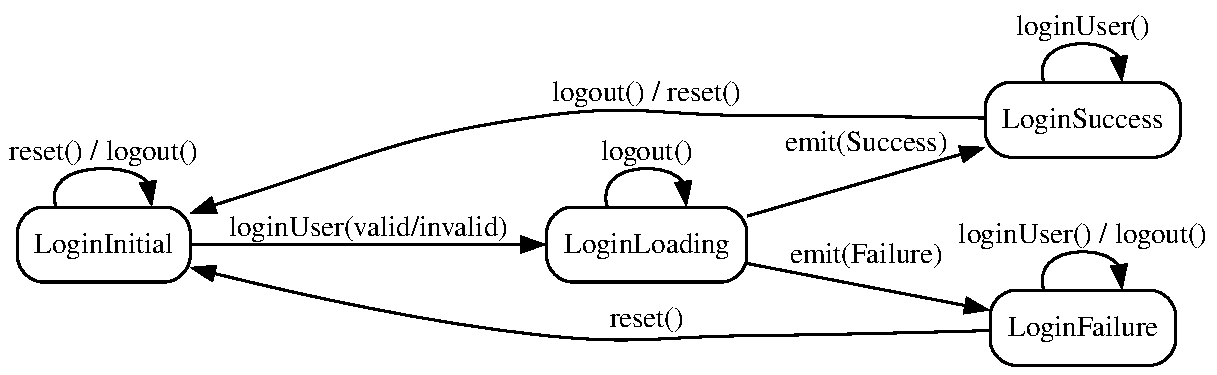
\includegraphics[width=0.8\textwidth]{dot/login.pdf}
\caption{Пример графа автомата состояний для гипотетического LoginCubit.}
\label{fig:cubit_fsm_example}
\end{figure}

\vspace{2cm}

\begin{figure}[!htb]
\centering
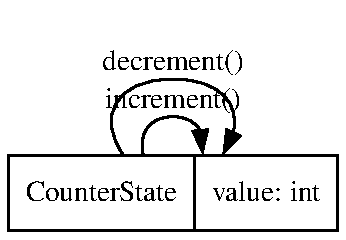
\includegraphics[width=0.7\textwidth]{dot/counter.pdf}
\caption{Пример графа автомата состояний для простого CounterCubit.}
\label{fig:cubit_fsm_example_2}
\end{figure}

% ================== ПРИЛОЖЕНИЕ В: ВЫПОЛНЕНИЕ ПРОГРАММЫ ДЛЯ БЛОКА ==================
\newpage
\anonsection{ПРИЛОЖЕНИЕ В}

В данном приложении представлены изображения генеративного информационного файла, при вызове генерации тестов для \texttt{auth\_login\_bloc}.

\begin{figure}[!htb]
\centering
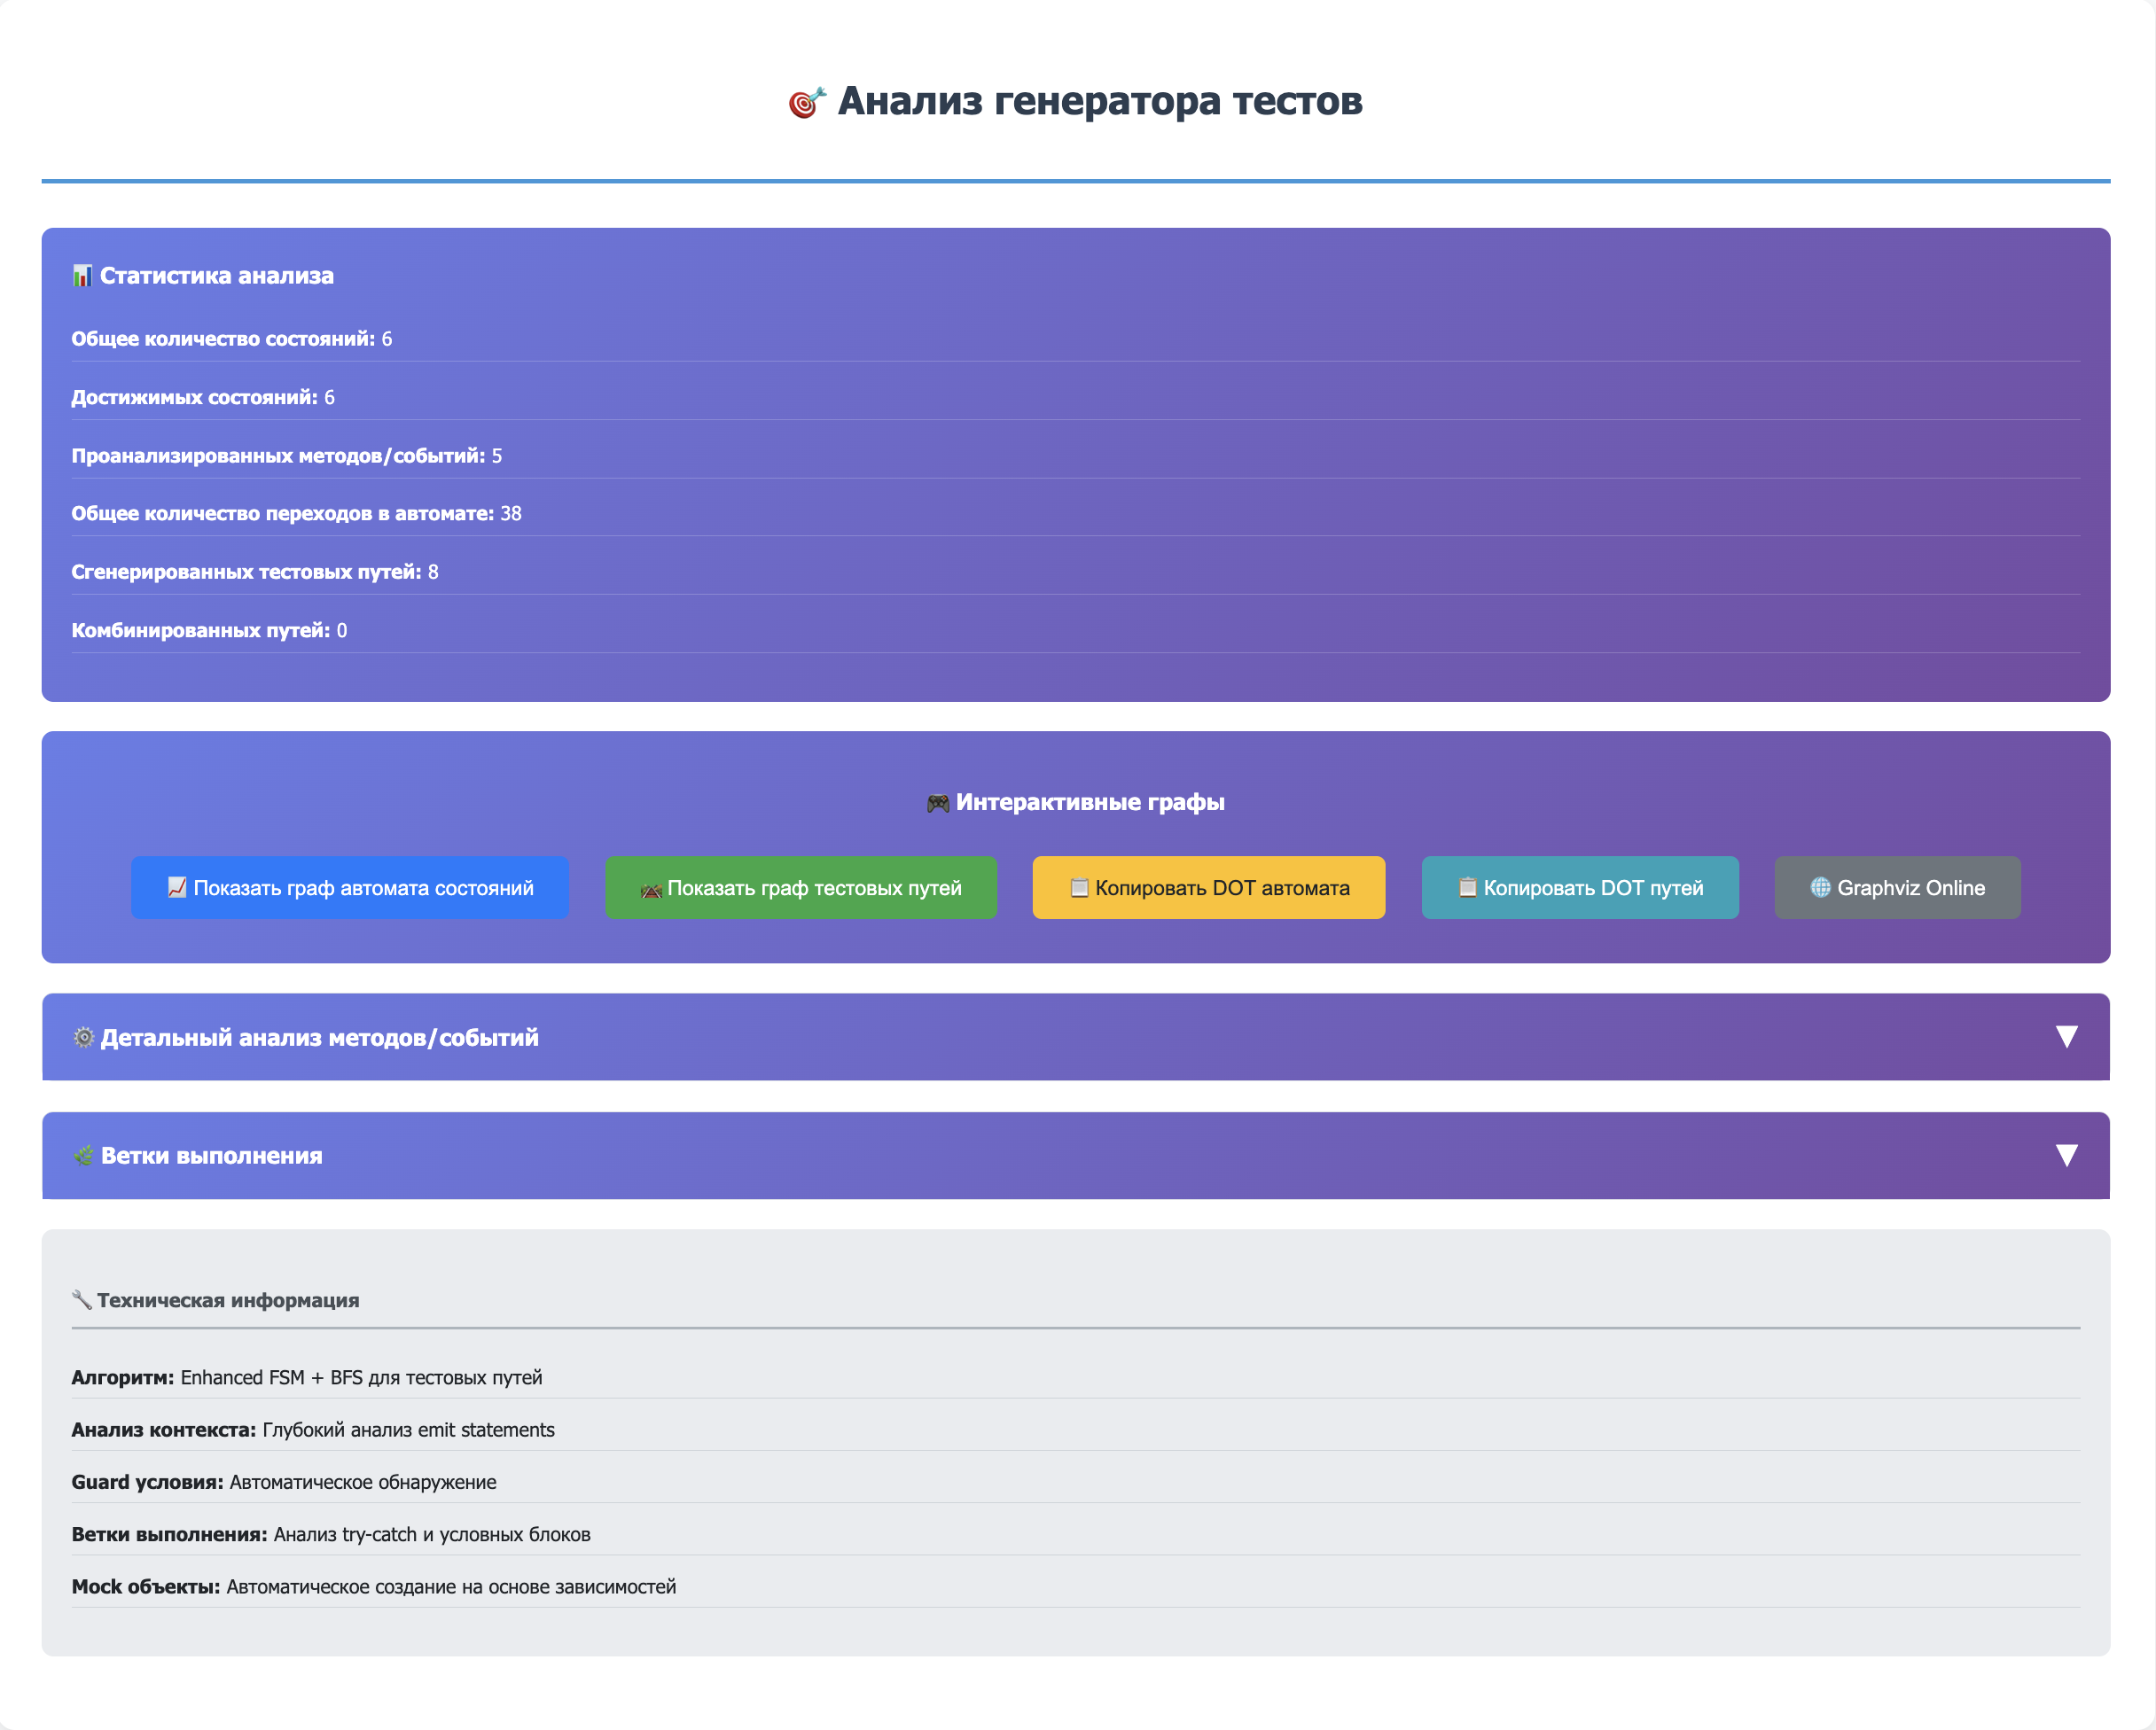
\includegraphics[width=0.8\textwidth]{images/bloc_1.png}
\caption{Общая информация о блоке.}
\label{fig:bloc_info}
\end{figure}

\vspace{2cm}

\begin{figure}[!htb]
\centering
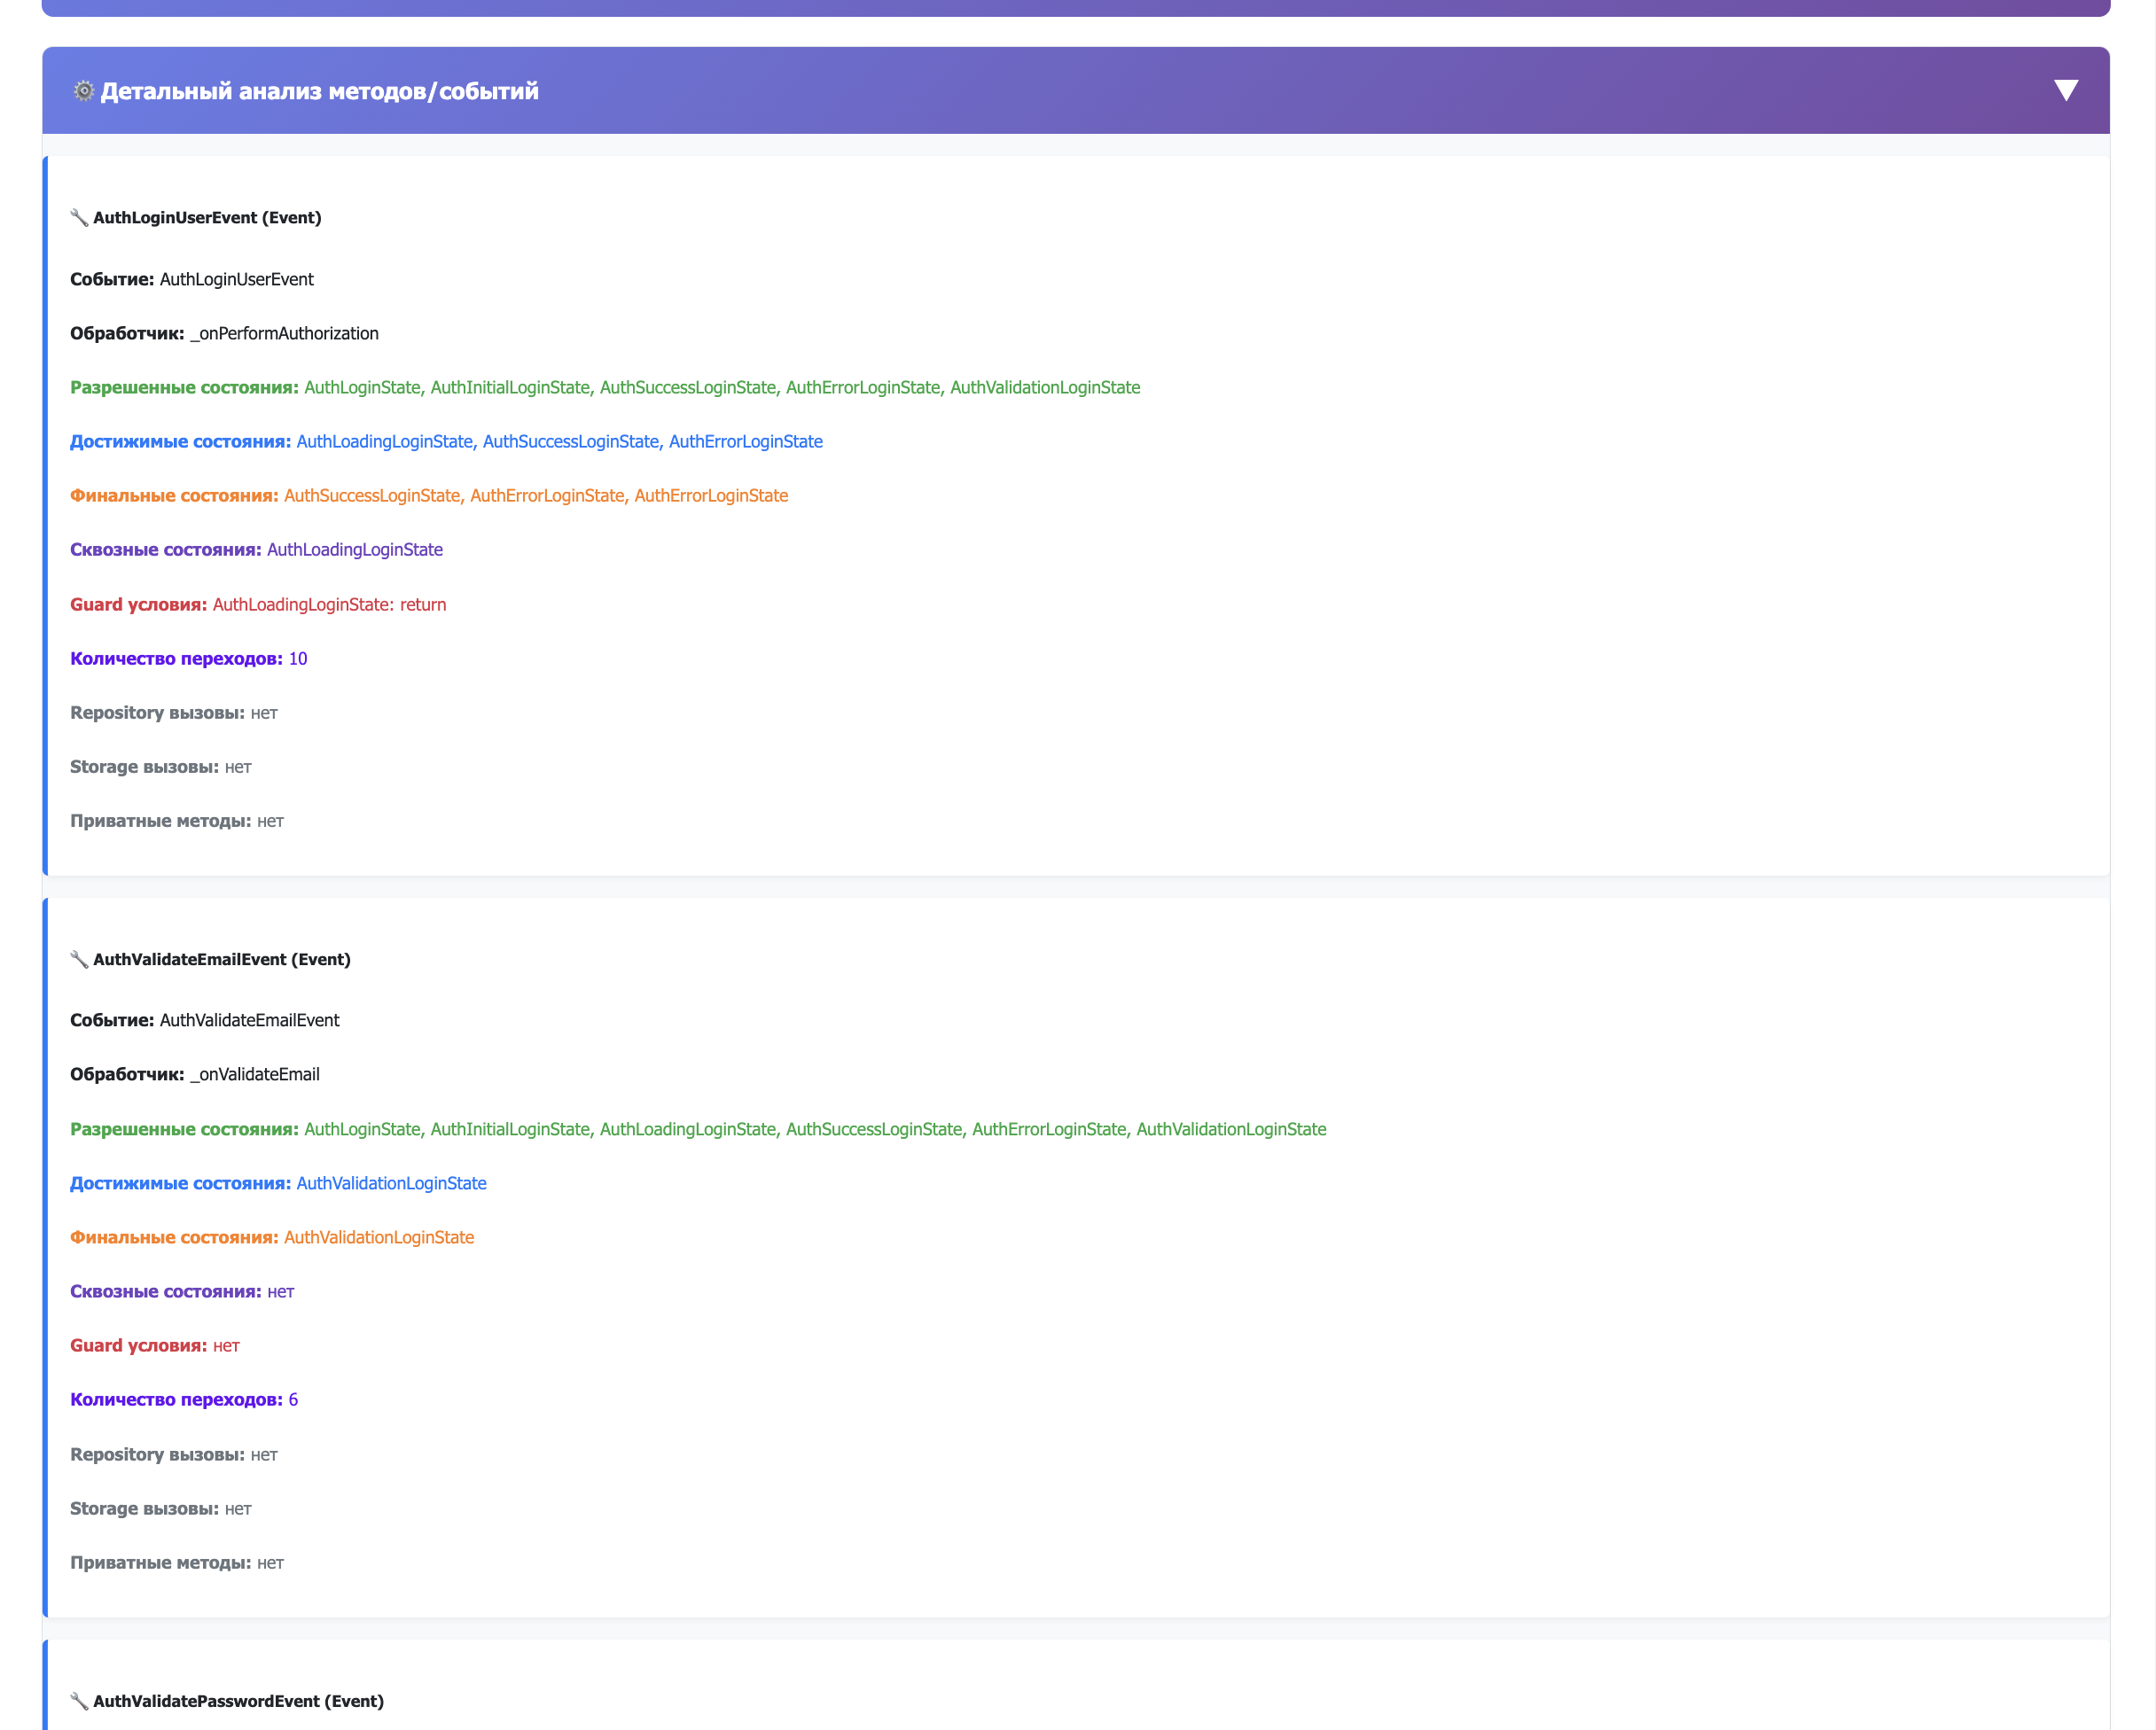
\includegraphics[width=0.7\textwidth]{images/bloc_2.png}
\caption{Информация об ивентах блока.}
\label{fig:bloc_test_info}
\end{figure}

\vspace{2cm}

\begin{figure}[!htb]
\centering
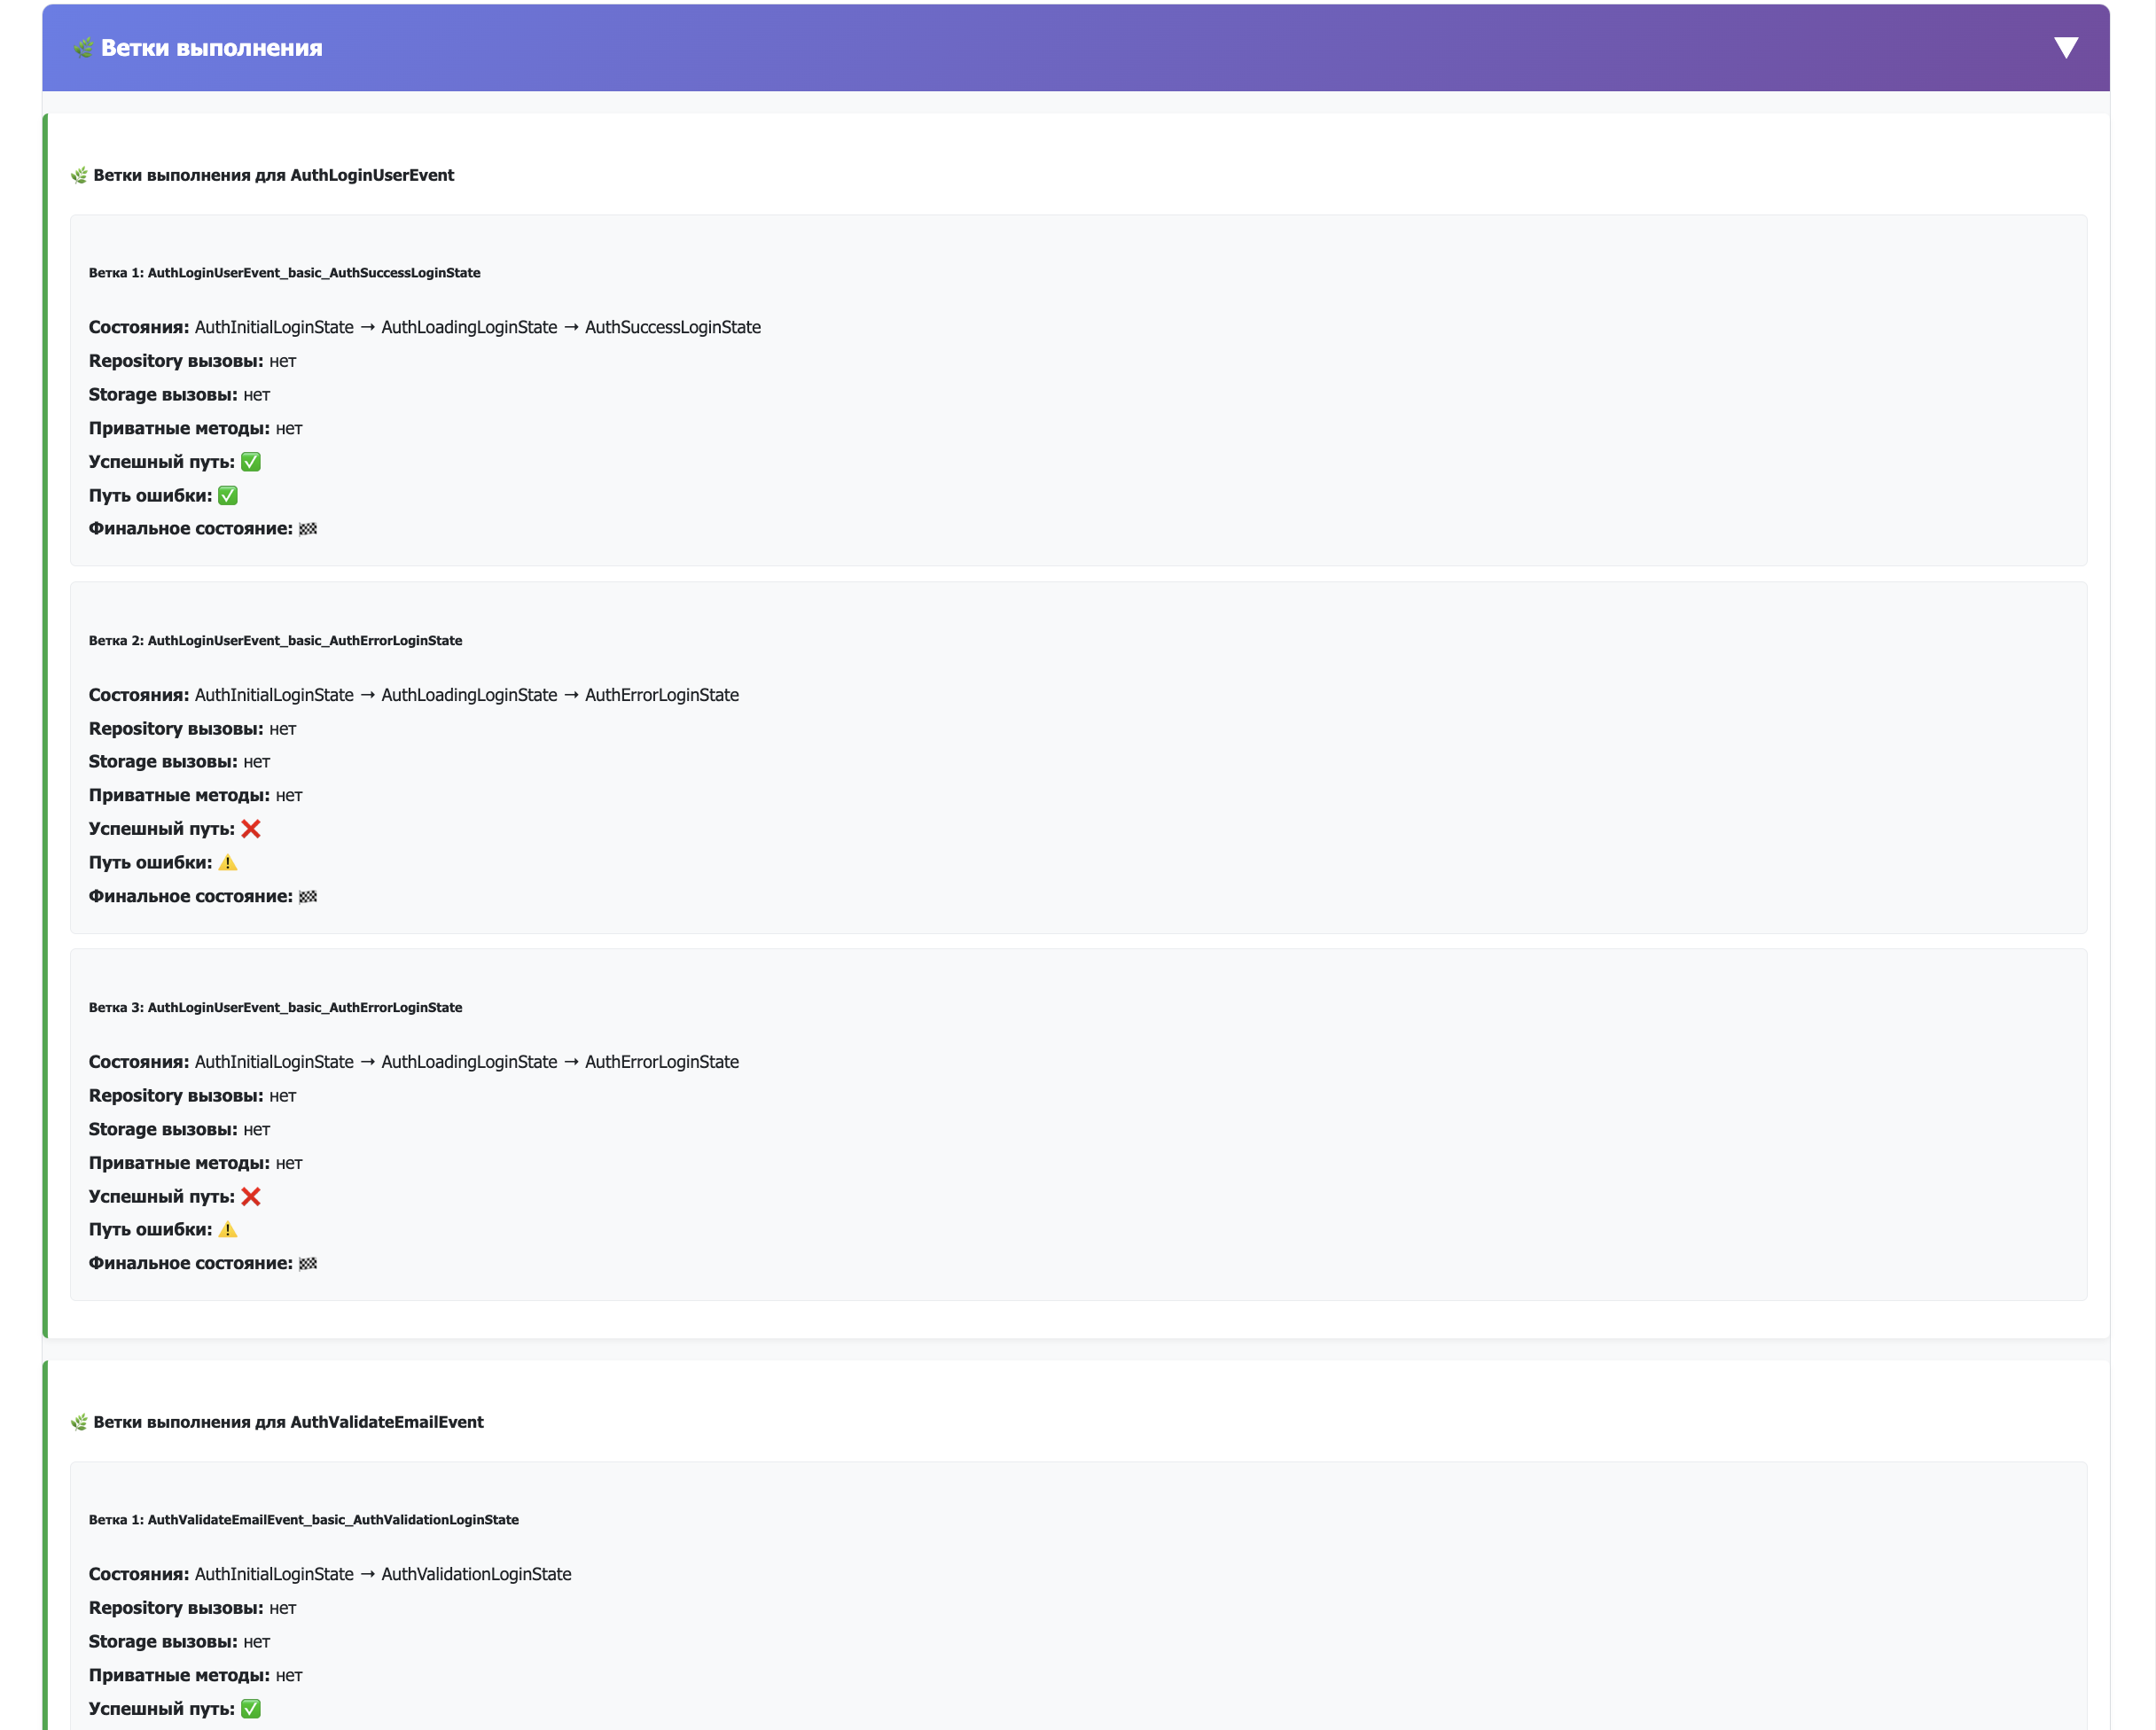
\includegraphics[width=0.8\textwidth]{images/bloc_3.png}
\caption{Информация о тестах блока.}
\label{fig:bloc_automat_1}
\end{figure}

\vspace{2cm}

\begin{figure}[!htb]
\centering
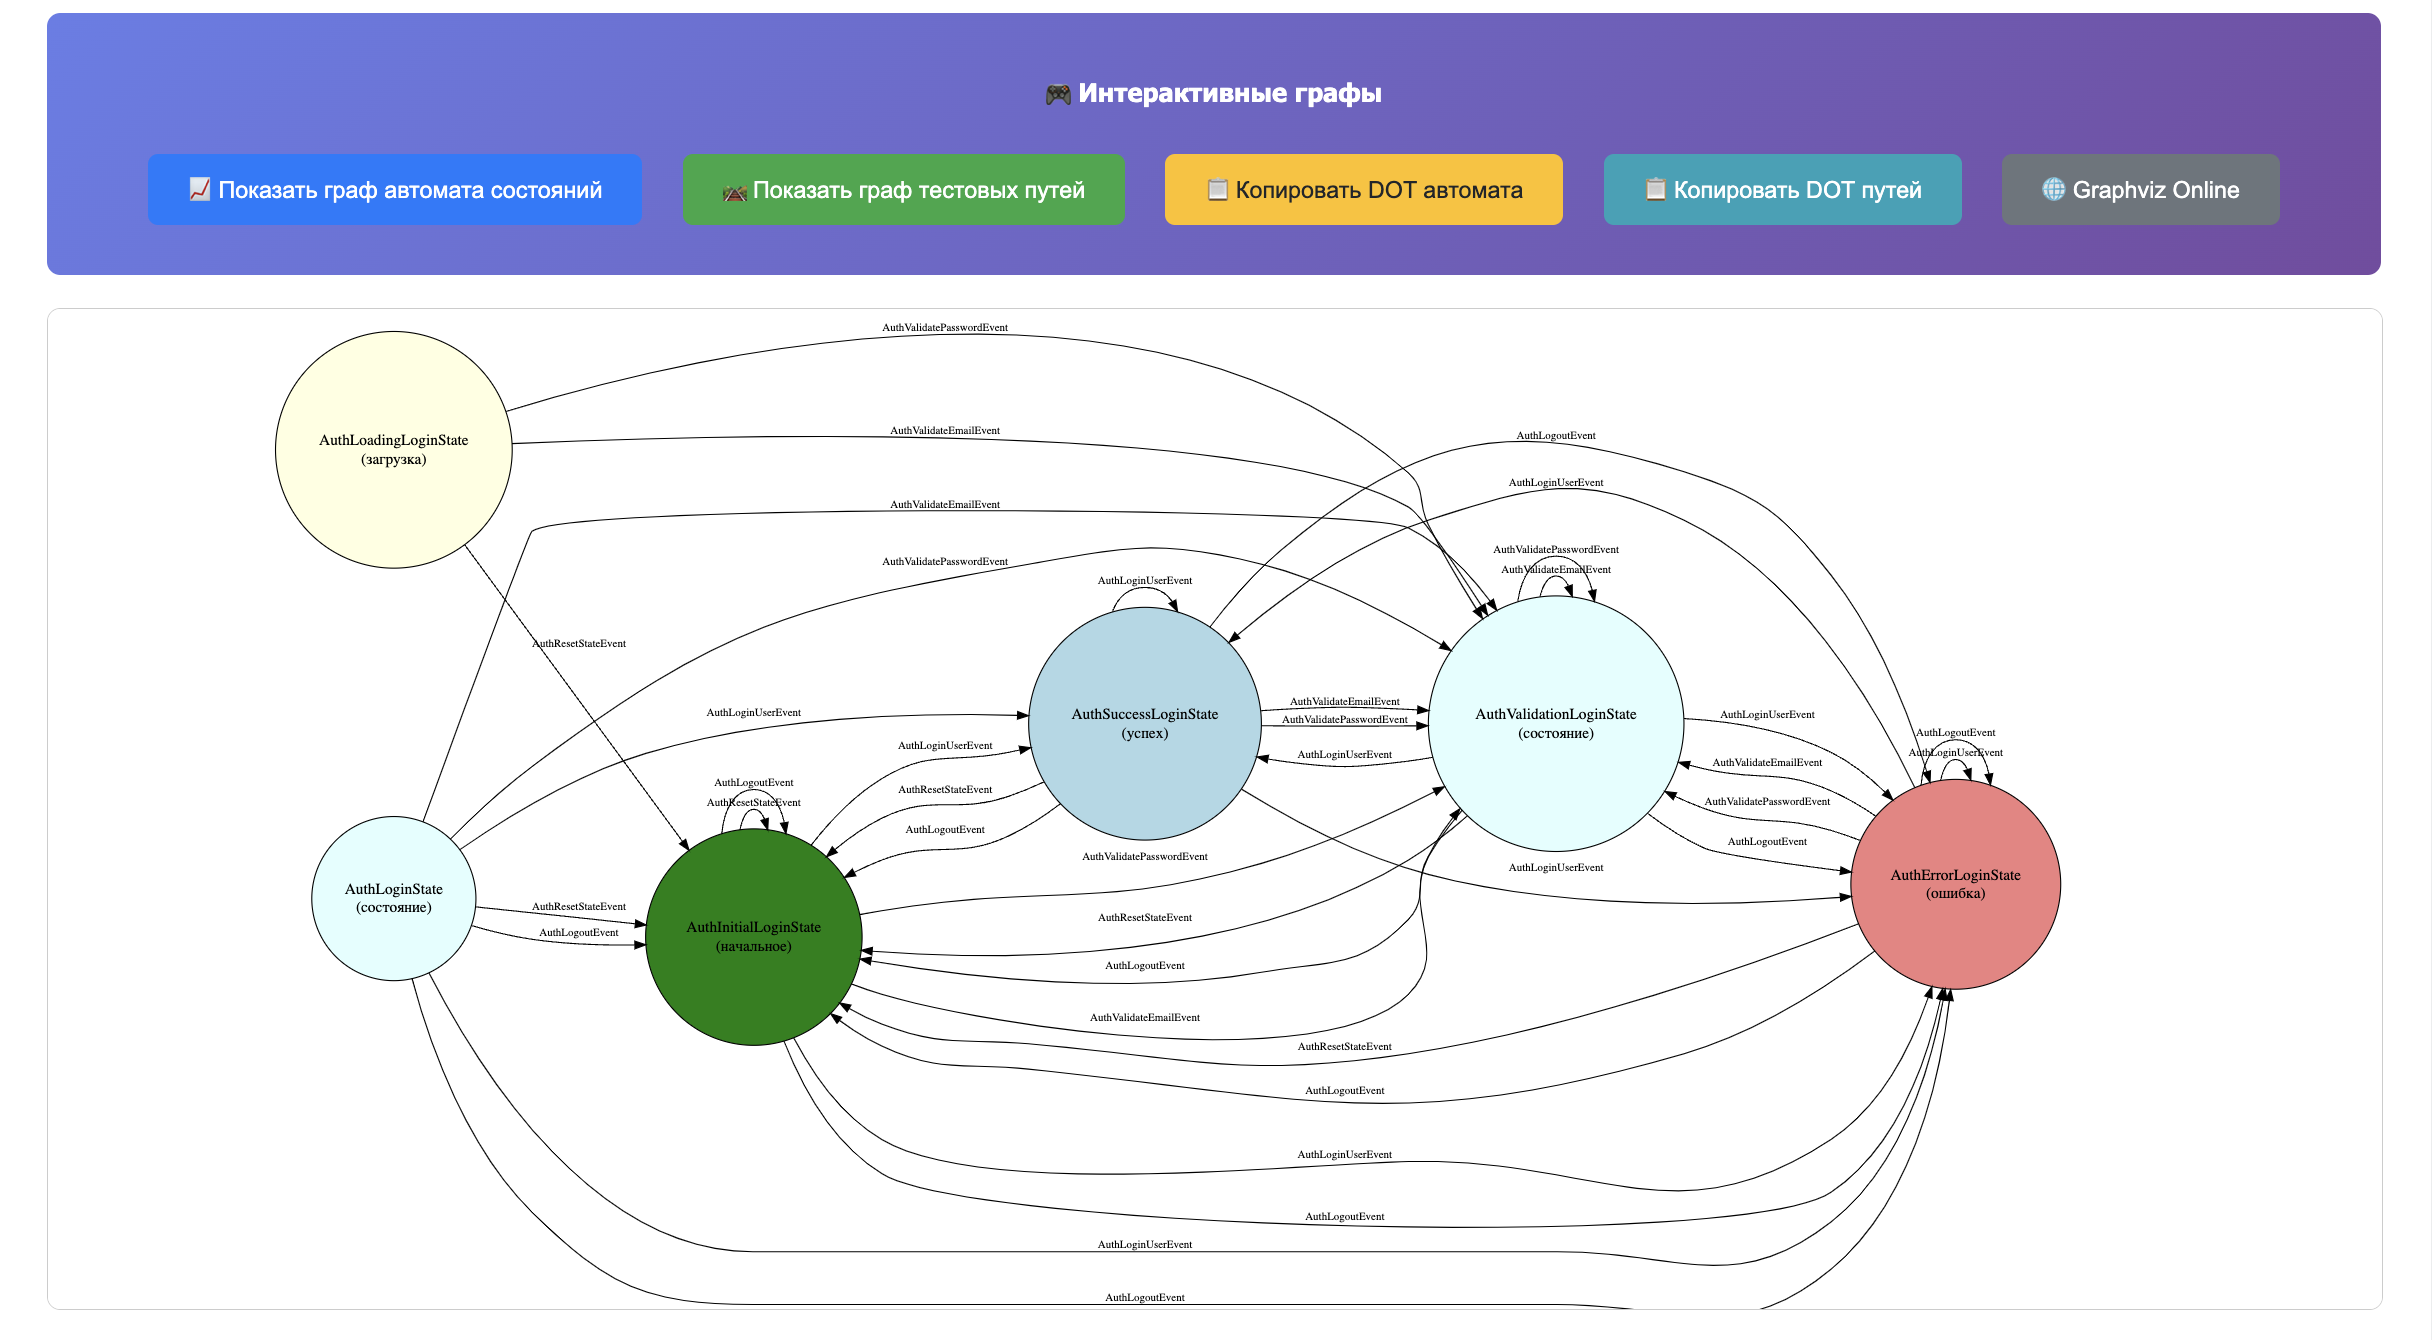
\includegraphics[width=0.7\textwidth]{images/bloc_4.png}
\caption{Атомат состояний блока.}
\label{fig:bloc_automat_2}
\end{figure}

\vspace{2cm}

\begin{figure}[!htb]
\centering
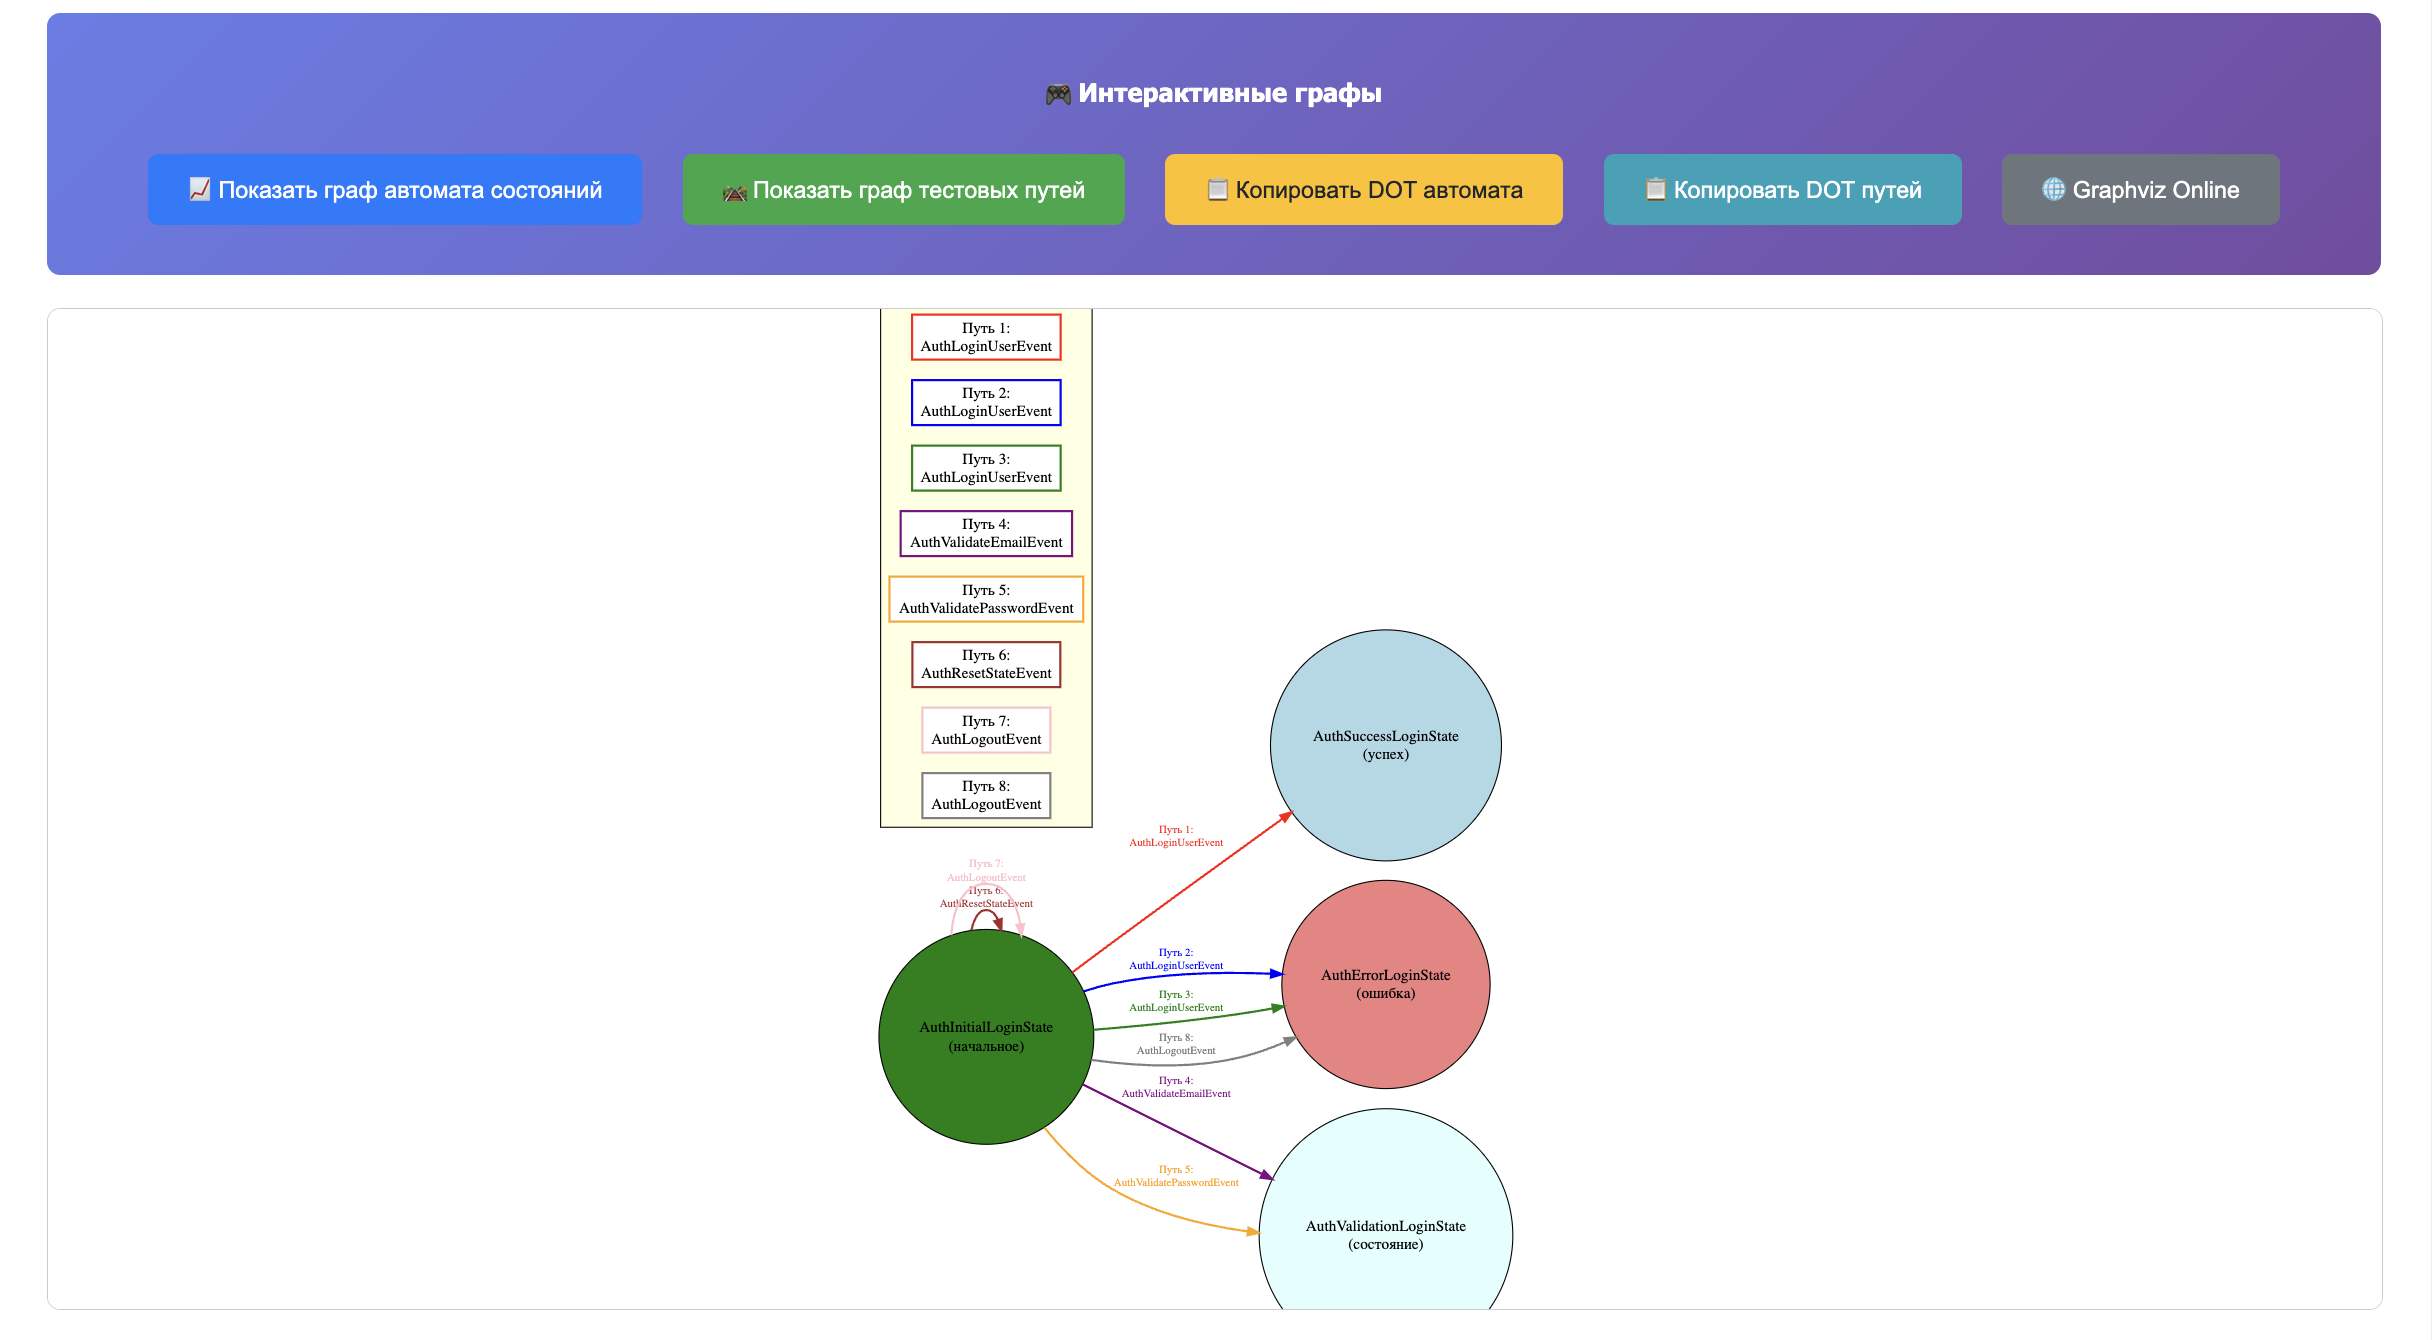
\includegraphics[width=0.7\textwidth]{images/bloc_5.png}
\caption{Тестовые множества блока.}
\label{fig:bloc_more_info}
\end{figure}

% ================== ПРИЛОЖЕНИЕ Г: ВЫПОЛНЕНИЕ ПРОГРАММЫ ДЛЯ КУБИТА ==================
\newpage
\anonsection{ПРИЛОЖЕНИЕ Г}

В данном приложении представлены изображения генеративного информационного файла, при вызове генерации тестов для \texttt{notification\_toggle\_cubit}.

\begin{figure}[!htb]
\centering
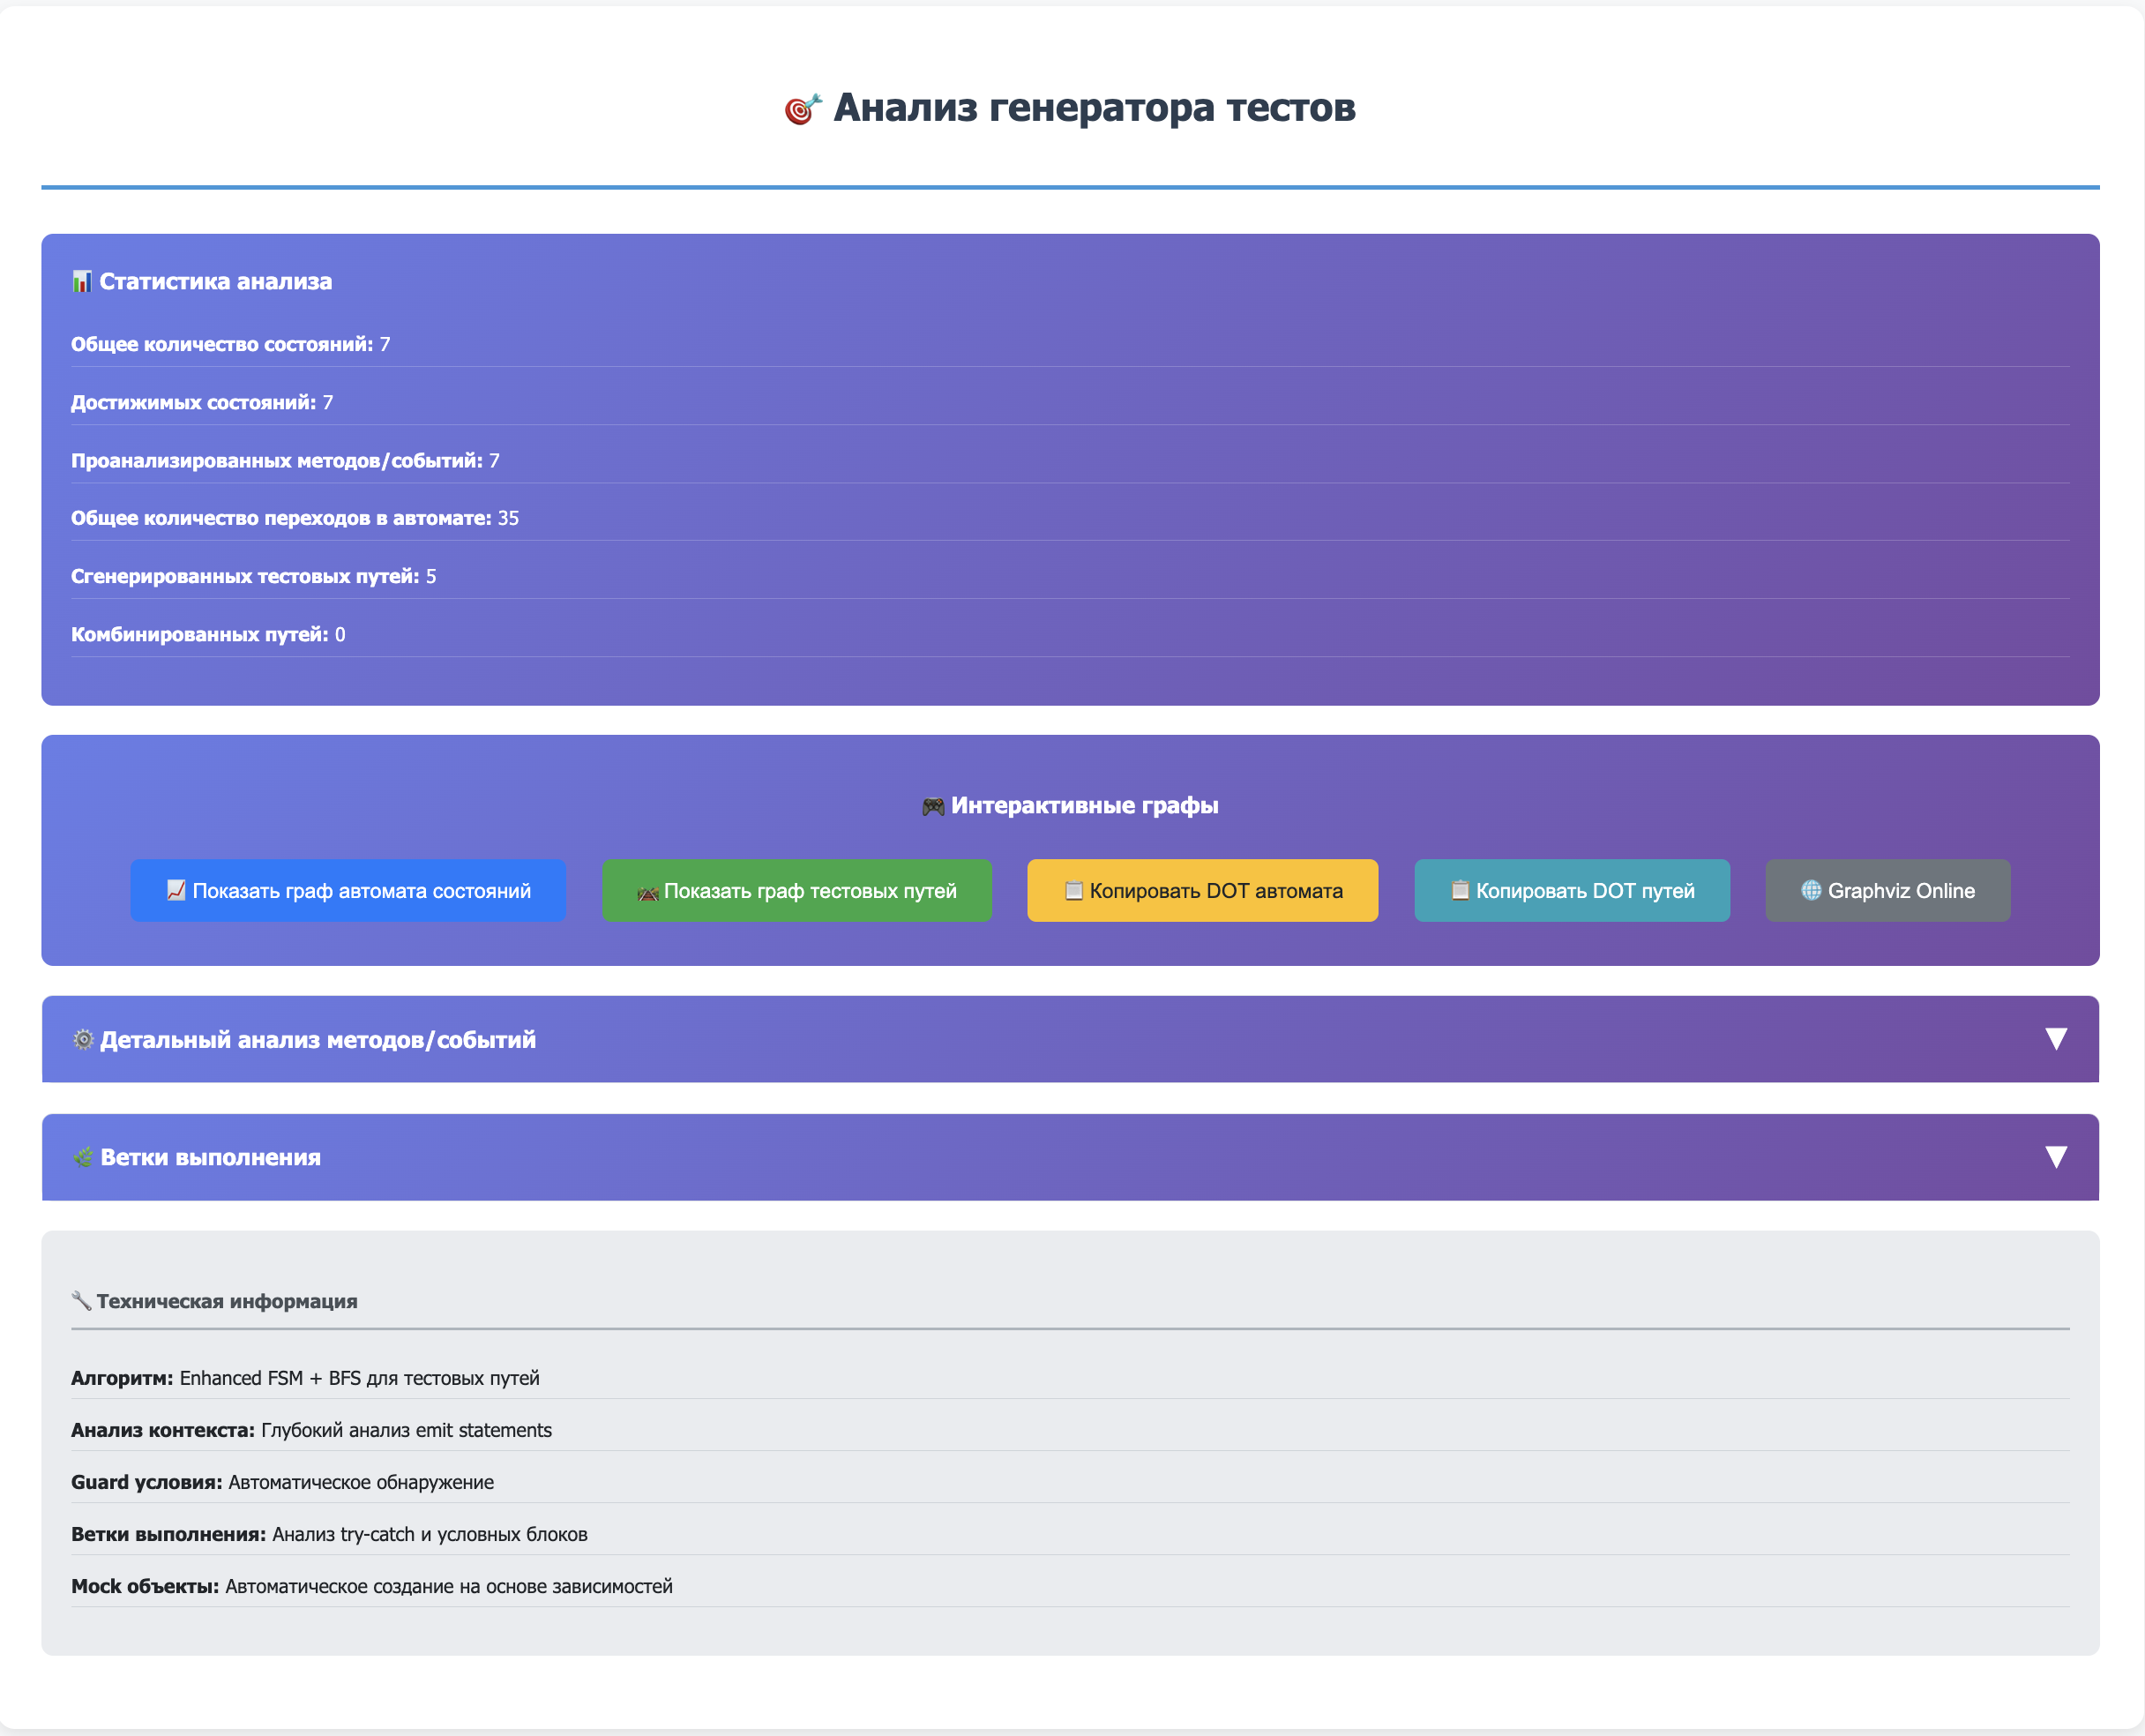
\includegraphics[width=0.8\textwidth]{images/cubit_1.png}
\caption{Общая информация о кубите.}
\label{fig:cubit_info}
\end{figure}

\vspace{2cm}

\begin{figure}[!htb]
\centering
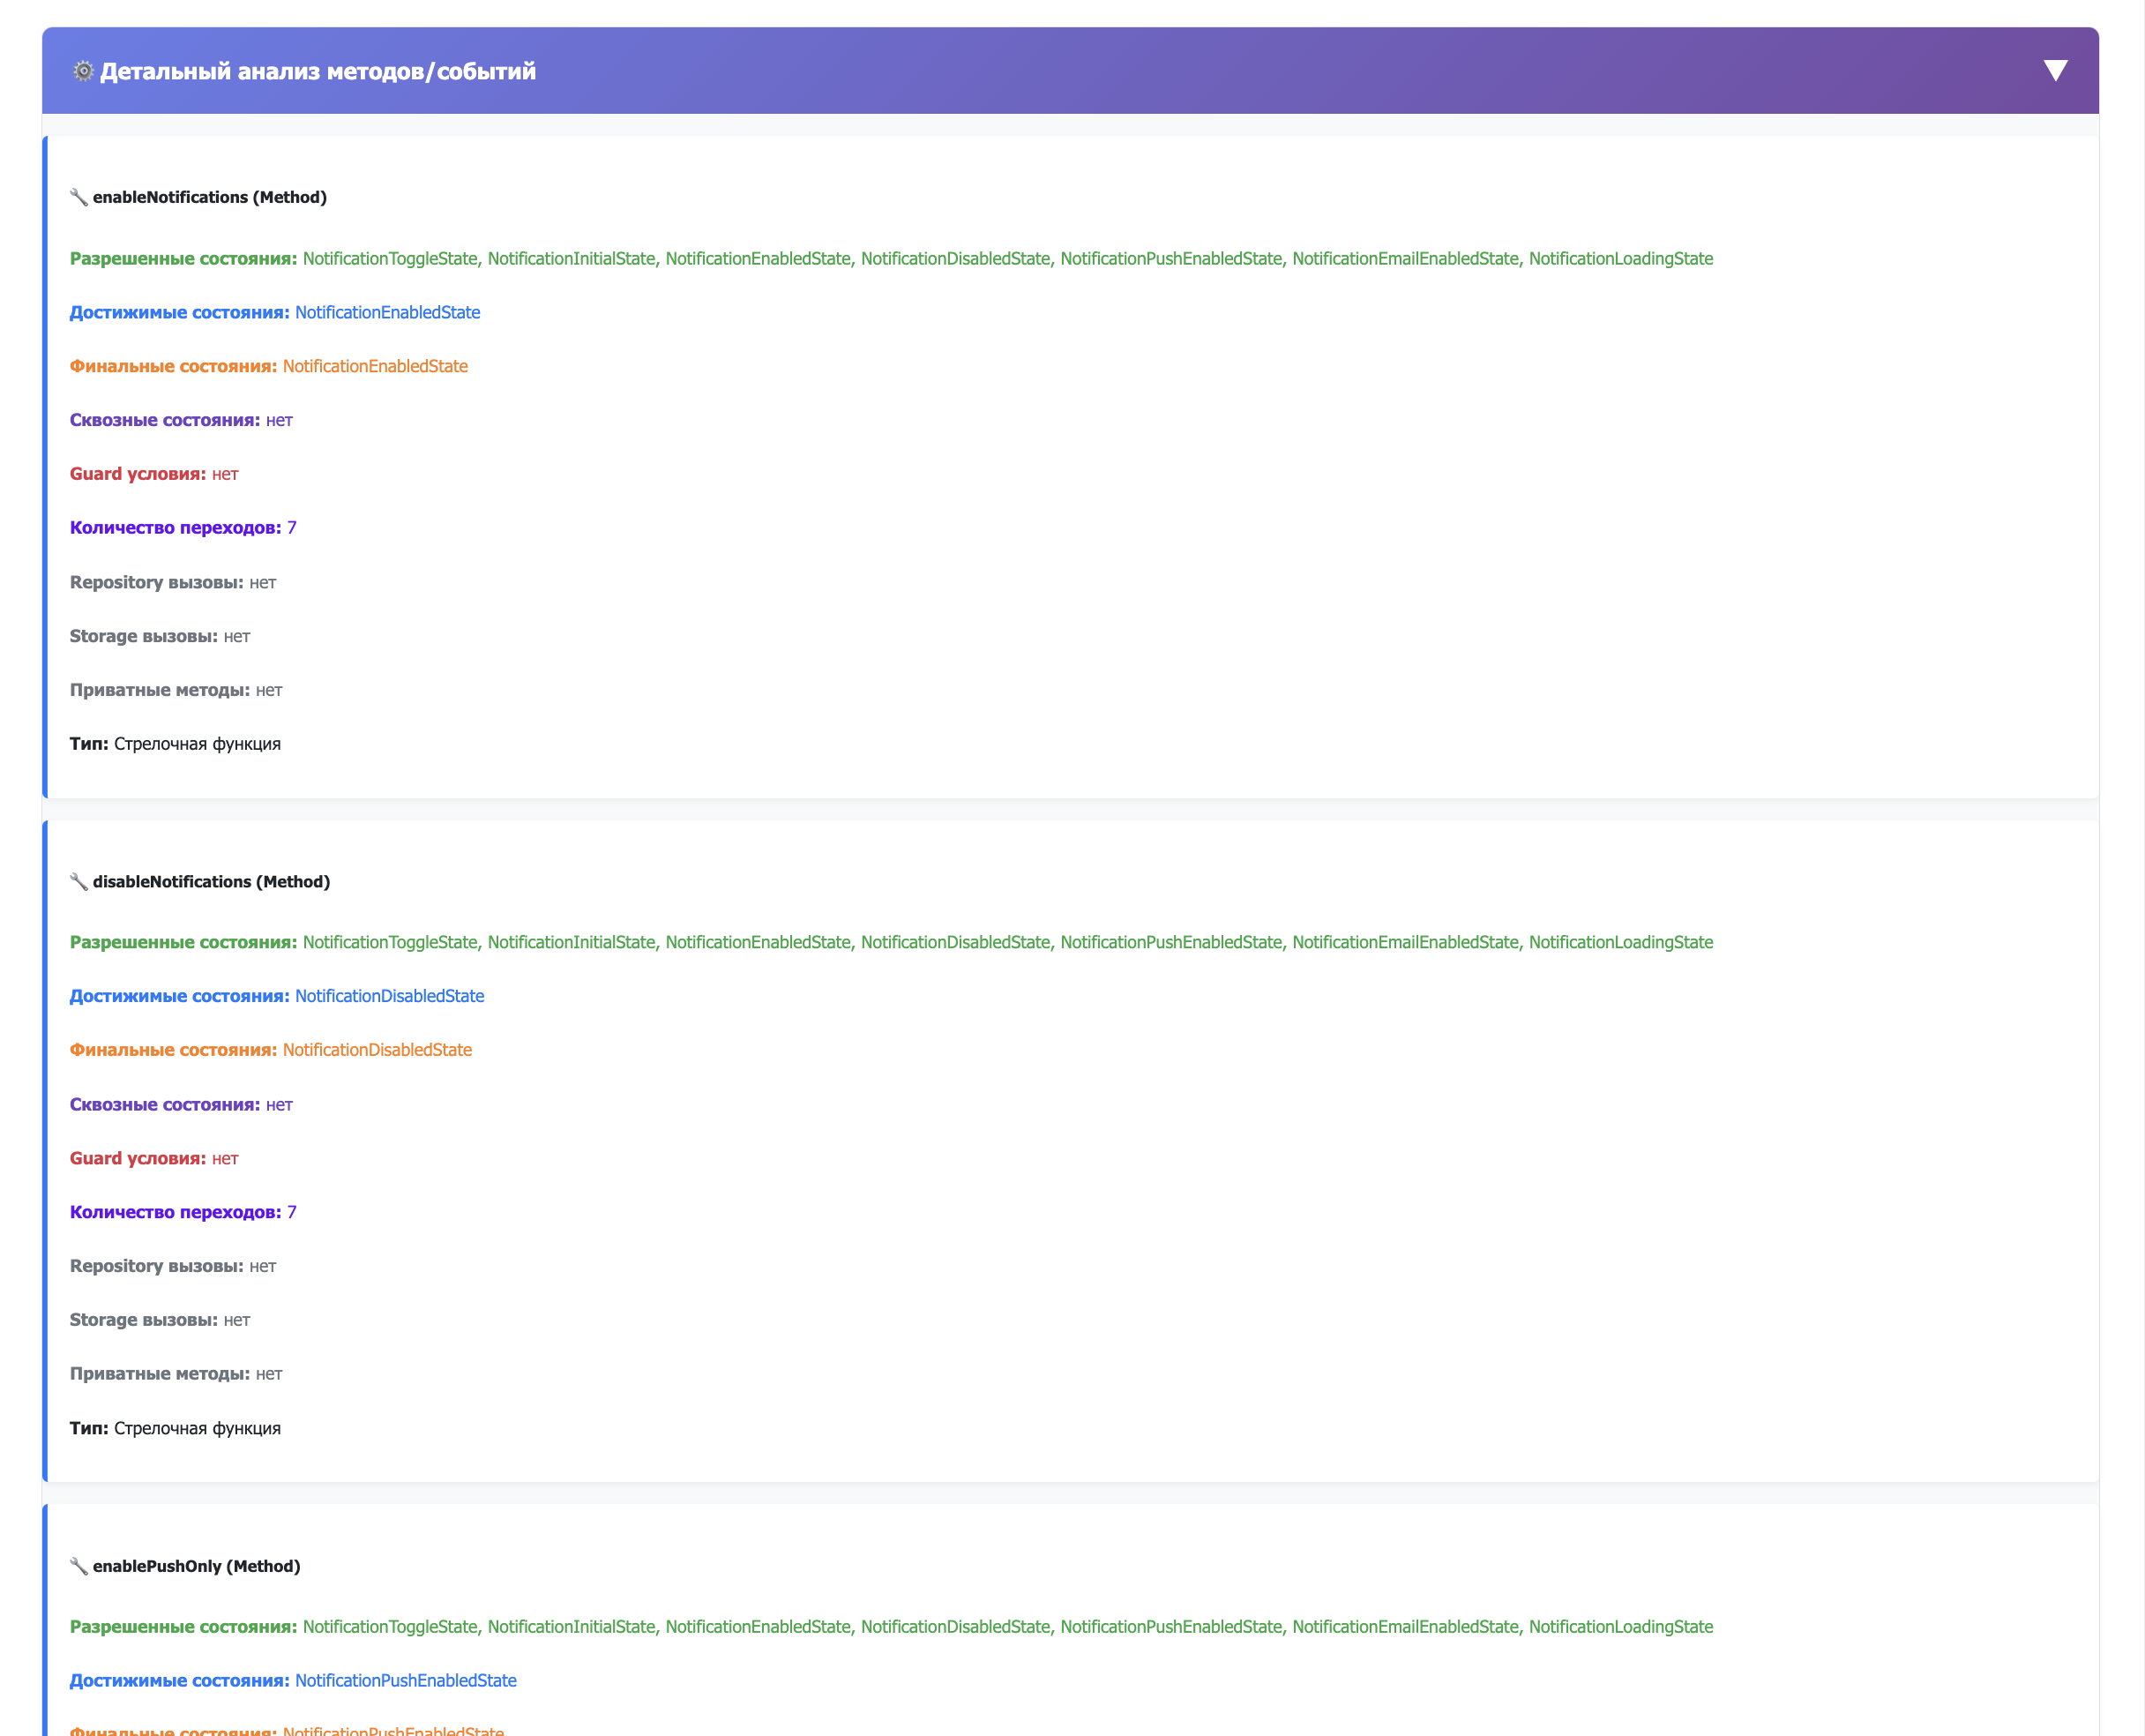
\includegraphics[width=0.7\textwidth]{images/cubit_2.png}
\caption{Информация о методах кубита.}
\label{fig:cubit_test_info}
\end{figure}

\vspace{2cm}

\begin{figure}[!htb]
\centering
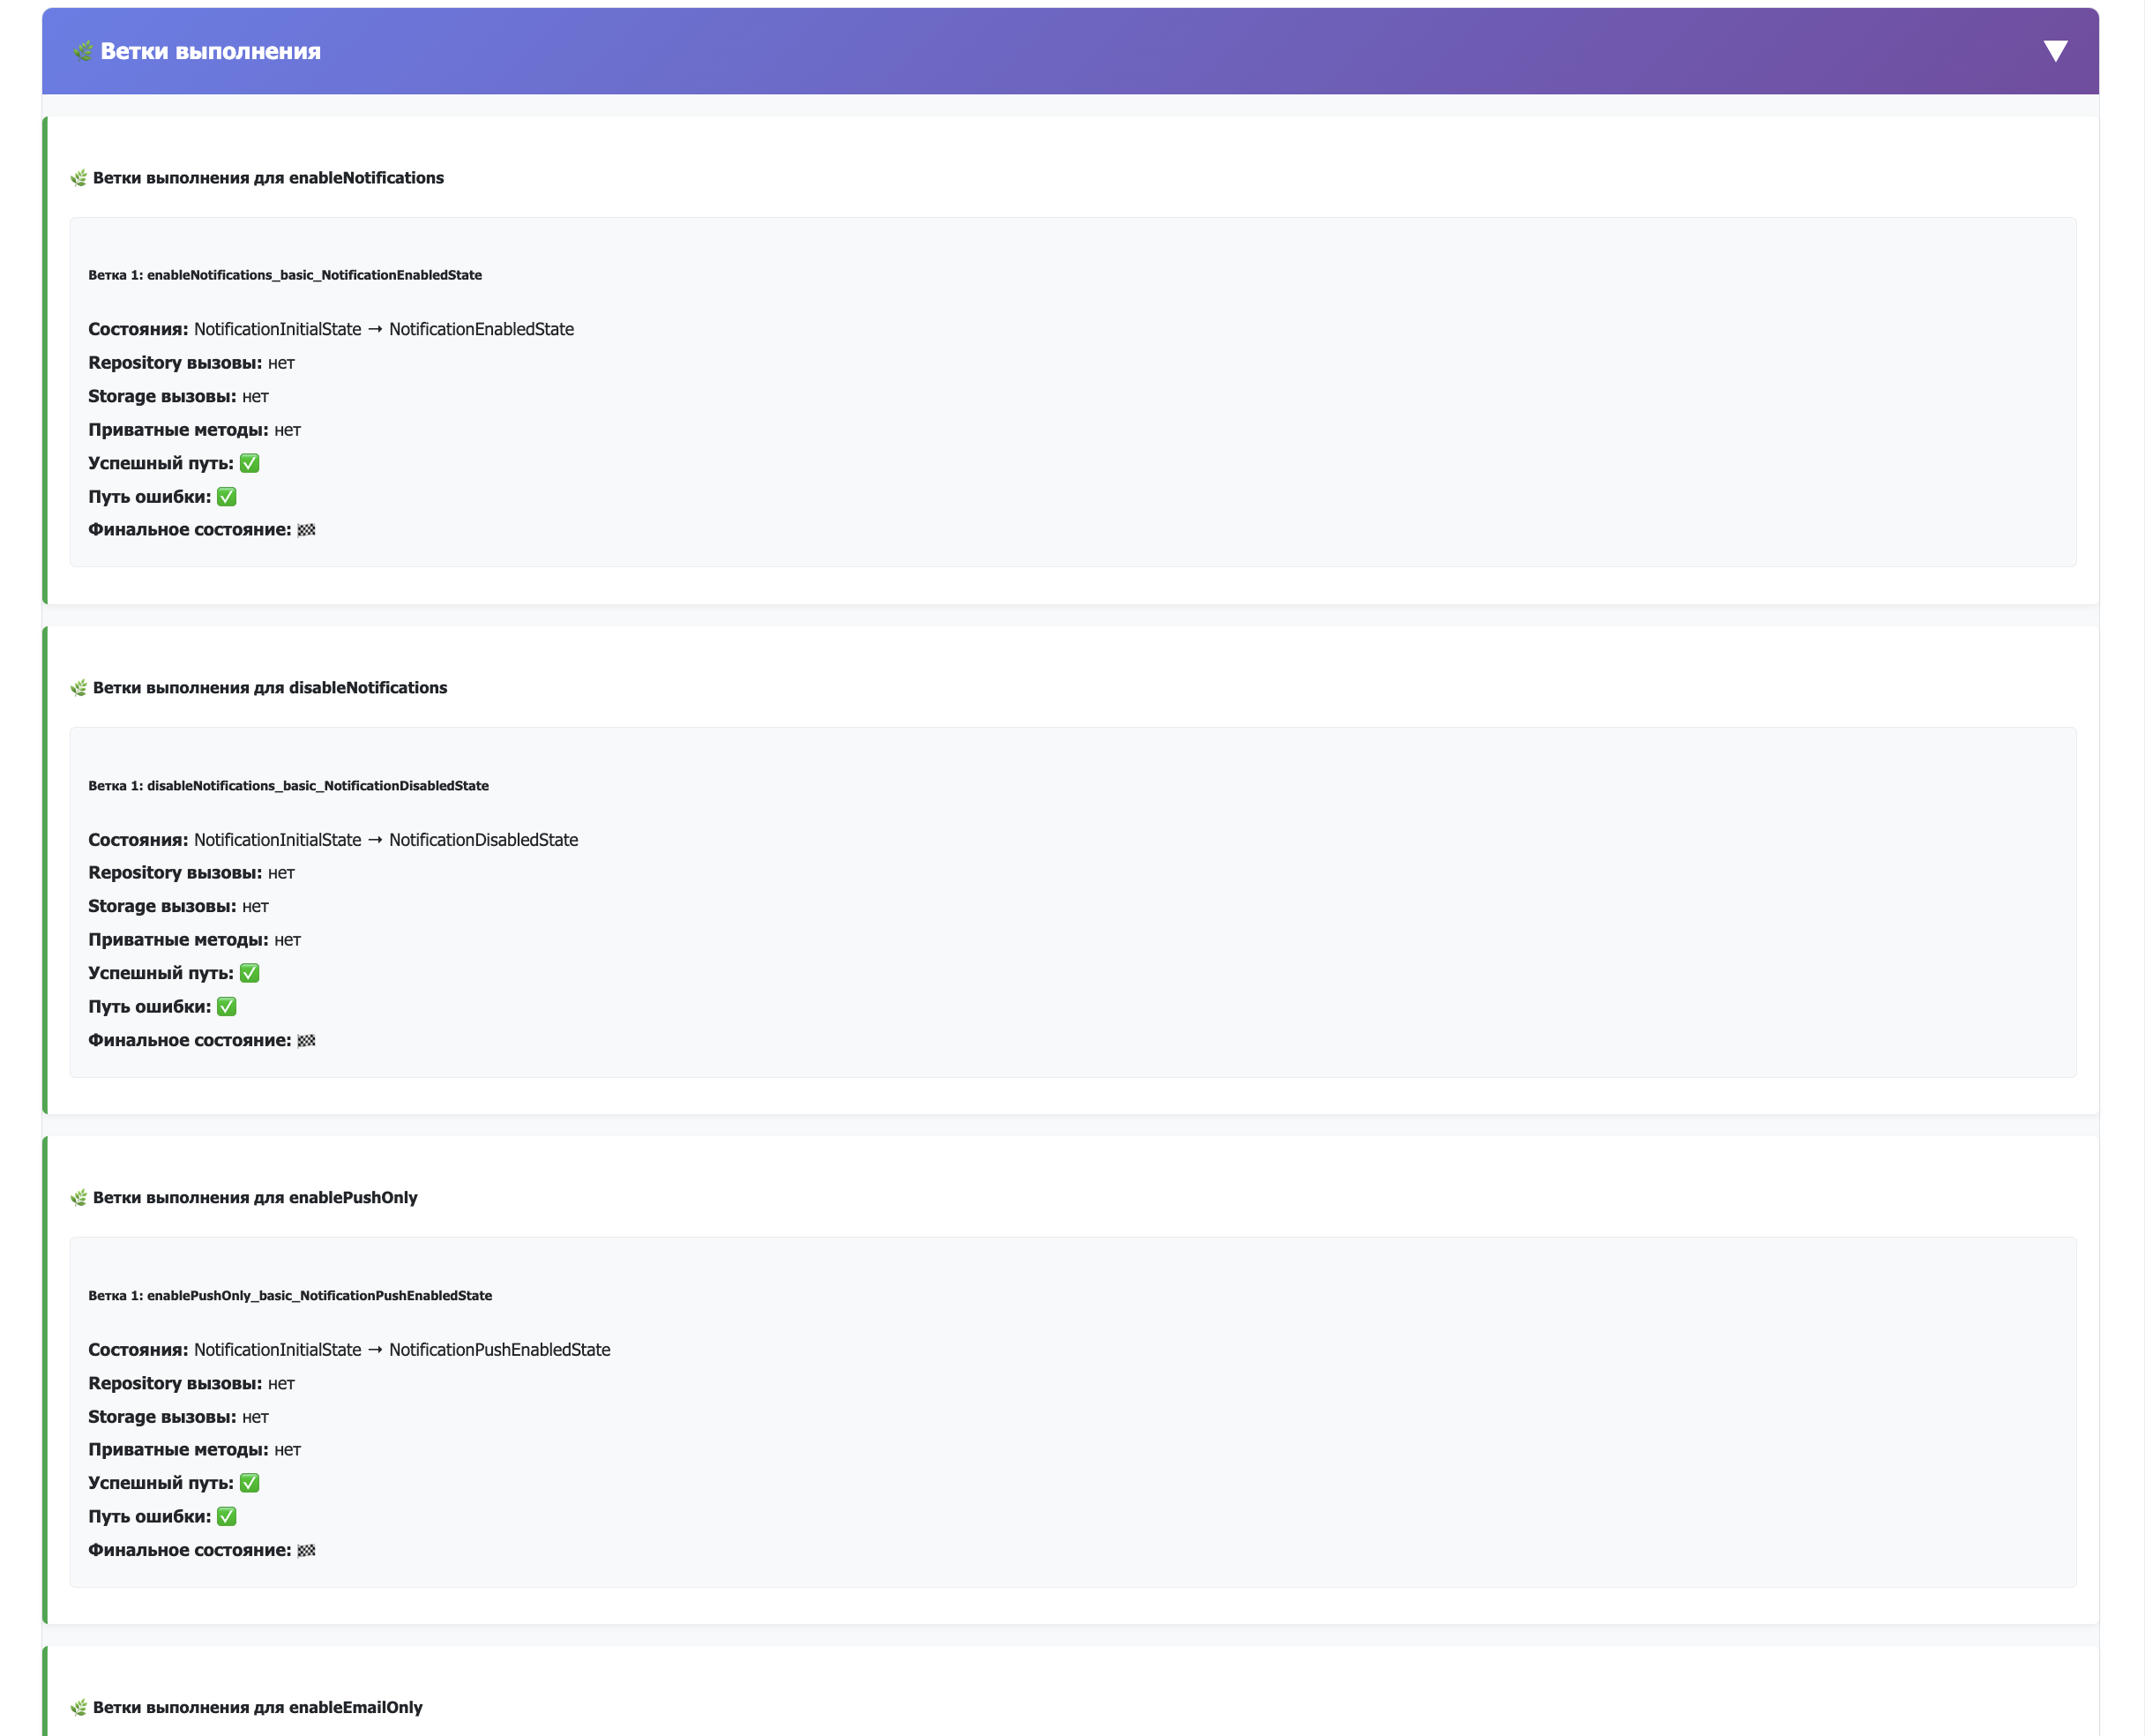
\includegraphics[width=0.8\textwidth]{images/cubit_3.png}
\caption{Информация о тестах кубита.}
\label{fig:cubit_automat}
\end{figure}

\vspace{2cm}

\begin{figure}[!htb]
\centering
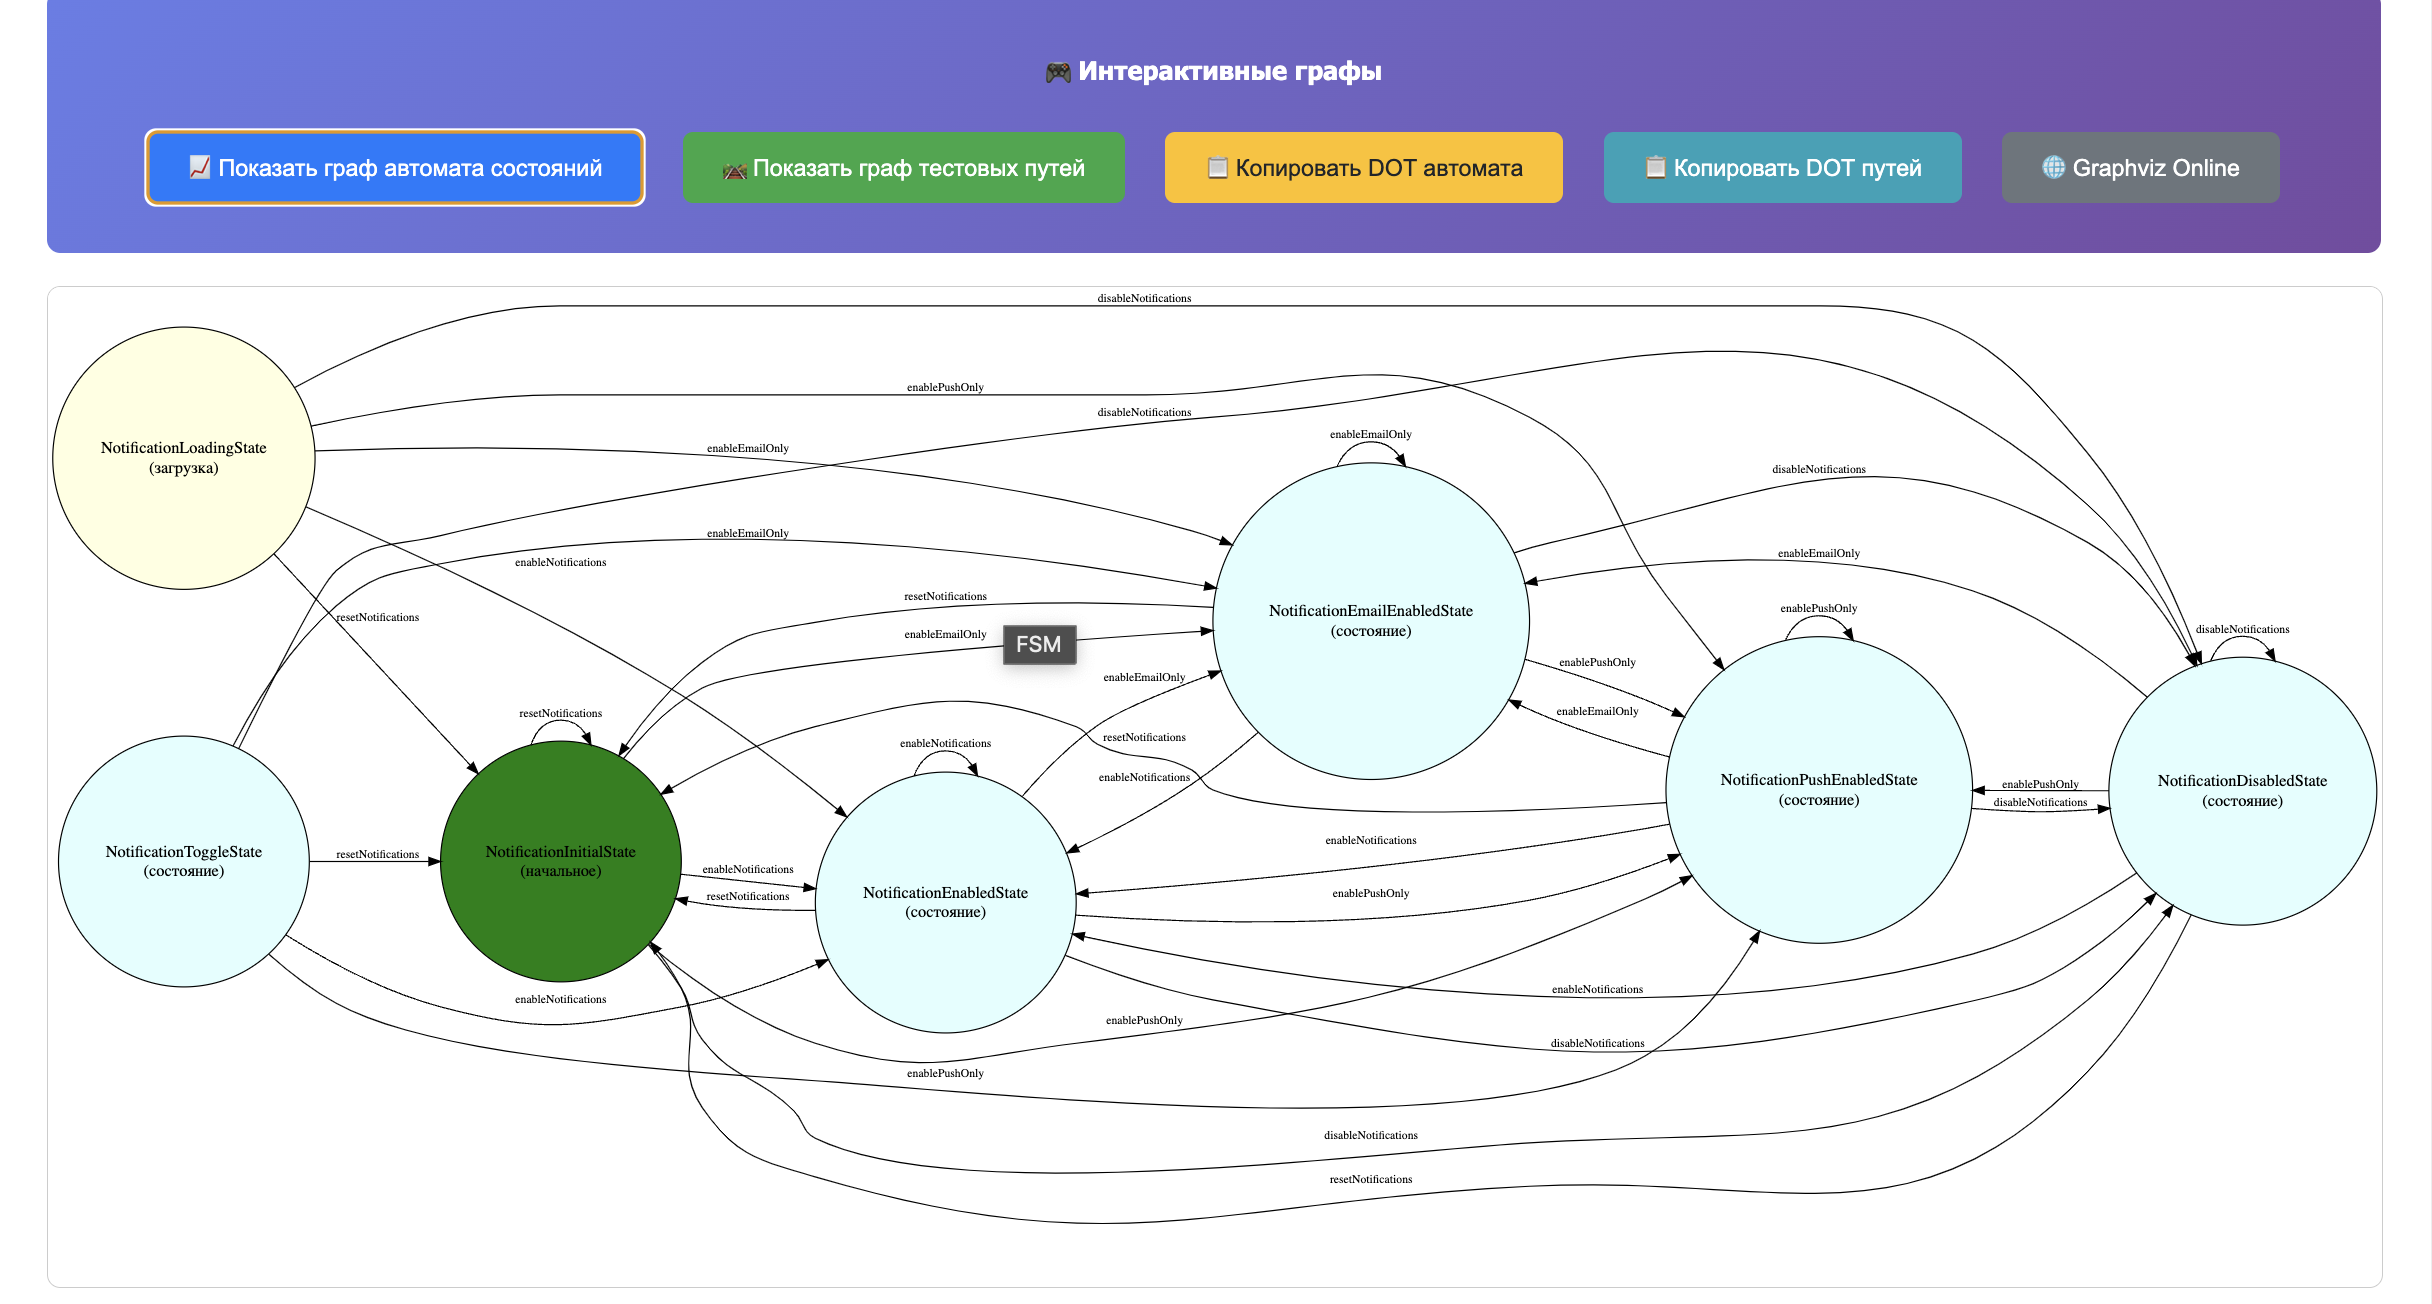
\includegraphics[width=0.7\textwidth]{images/cubit_4.png}
\caption{Атомат состояний кубита.}
\label{fig:cubit_more_info}
\end{figure}

\vspace{2cm}

\begin{figure}[!htb]
\centering
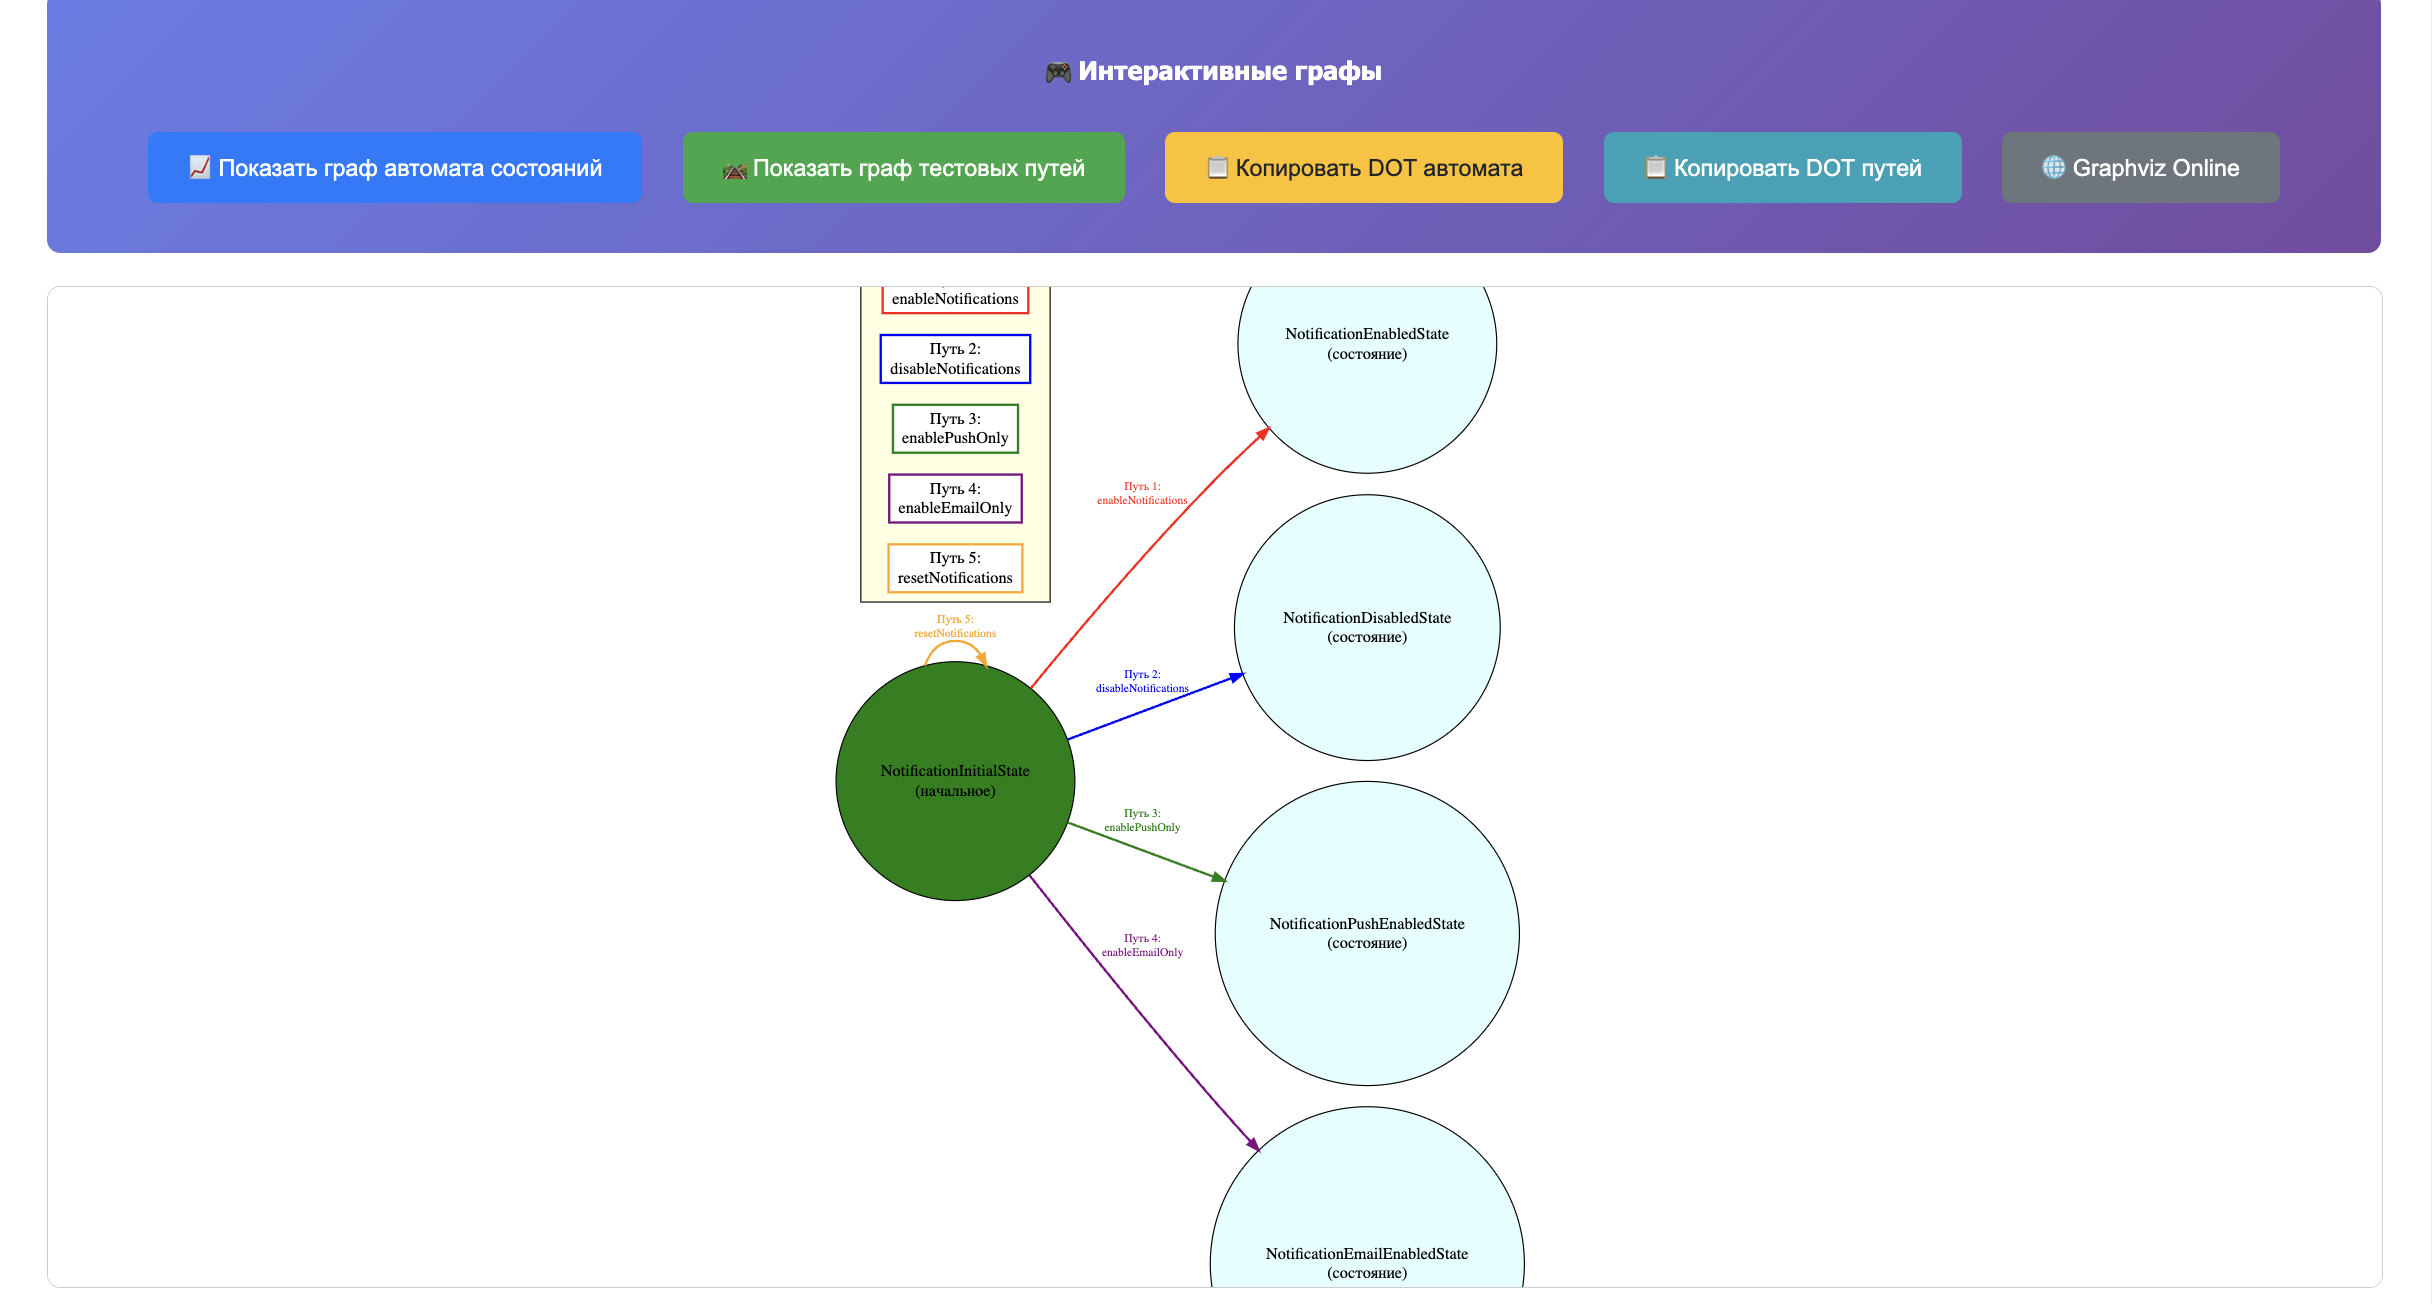
\includegraphics[width=0.7\textwidth]{images/cubit_5.png}
\caption{Тестовые множества кубита.}
\label{fig:cubit_more_info}
\end{figure}

% Конец отчета
\end{document}
